\section{PLL Architecture}\label{pll_arch}
To meet the goals of this work to achieve state of art power consumption of $\leq 100\mu$W for 2.448 GHz operation, while maintaining better than 20.56 ps RMS of phase jitter, the PLL architecture of figure figure \ref{fig:pll_arch} has been devised. It comprises primarily of three main components:
\begin{enumerate}[itemsep=0pt,label=\protect\mycirc{\arabic*}]
	\setlength\itemsep{-0.8em}
	\item A bang-bang phase detector.
	\item An all digital proportional-integral controller loop filter.
	\item A DCO implemented as a VCO digitized by capacitive DACs.
\end{enumerate}
The high level rationale for this architecture will be described in the following subsections. Furthermore, section \ref{sec:pd_design} details the design and implementation of the phase detector, section \ref{sec:design_lf} details the design and implementation of the loop filter, and section \ref{sec:dco_design} describes the design and implementation of the DCO.

	\subsection{Block Diagram}
			\begin{figure}[htb!]
		        \centering
		        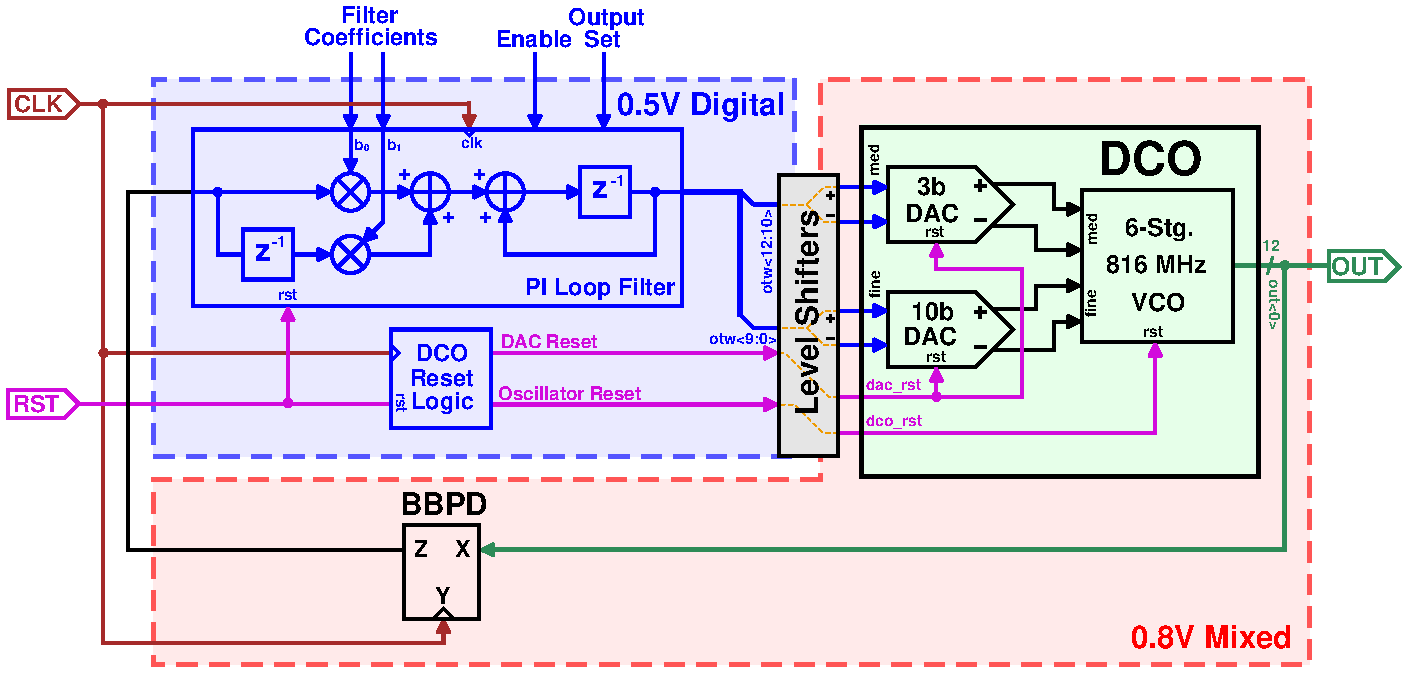
\includegraphics[width=1\textwidth, angle=0]{./figs/design/pll_master_arch_final3}
			    \caption{ADPLL Architecture.}
			    \label{fig:pll_arch}
			\end{figure}

	\subsection{Power Saving Driven Approach}
	The general design philosophy of this work is tailored to save power by pursuing simplicity wherever possible. Reduction of complexity will reduce number of sources of power draw, and will also reduce noise generated due to fewer devices providing contributions. Several measures have been employed to these ends. First of which is the omission of a divider in this design. As will be later described, such a modification allows for reduction in phase noise contribution of the phase detector, and total removal of divider noise contributions. Furthermore, any power draw associated with the divider is avoided. The removal of the divider, however, requires that accurate calibration of the PLL frequency tuning range must be performed during cold start of the PLL. Implementation of such a calibration scheme should be expected to add minimal power consumption as any excess calibration circuitry required can be disabled during normal operation. Additional power improvements are obtained in the usage of digital logic to implement the loop filter in this work, using a simple PI-controller architecture. As shown in figure \ref{fig:pll_arch}, the application of split power domains is used, with supplies of (a) 0.5V for loop filter, and (b) 0.8V for the DCO and phase detector. The multiple power domains allows for reduction of the digital logic supply voltage to just the level needed for reliable operation, saving power, while allowing for sufficient voltage for proper oscillator function. The digital nature of the loop filter lends itself to low sensitivity to process, voltage, and temperature (PVT) variation, and is expected that compared to analog designs, a smaller margin of safety in the power can be employed to ensure satisfactory performance with variation. The final architectural power saving move is implemented in a DCO based on the combination of several CDACs with a voltage controlled ring oscillator. This reduces to near zero the DC current draw associated with control of the VCO. The resulting overall design is therefore implemented with no static current paths (other than that associated with leakage), in hopes of achieving better energy efficiency than designs that require extraneous power draw, for example in those that utilize current mirrors needing reference current generation.

	\subsection{PLL Sleep Capability}
	As motivated by the end application of this PLL to wake up receivers, the architecture of the PLL has been developed to support duty cycled operation. Specifically, the architecture has been designed to enable rapid locking, such that duty cycling at high frequencies can be performed with a small level of overhead for relocking of PLL when returning to an active state. This is implemented through the usage of an all-digital architecture, which allows for the PLL to save digitally the loop filter state when entering a sleep state. The implication of this is that all unneeded portions of the PLL may be powered down during inactive periods, saving power, and upon resuming to an on-state, the PLL can be restored rapidly to its pre-sleep state. If the time interval of sleep is sufficiently short, it is expected that the oscillator and supply characteristics will only drift minorly, thus the PLL will be either in a locked state, or near-locked state when it resumes from the stored state. Compared to restarting from a totally unlocked state (for example in a cold start up), the time spent locking is expected to be greatly reduced with this architectural decision. Figure \ref{fig:pll_sleep} demonstrates such operation described, where $t_{l1}$ is the lock time from cold start, and $t_{l2}$ is the time to relock from a resume state.

			\begin{figure}[htb!]
			        \centering
			        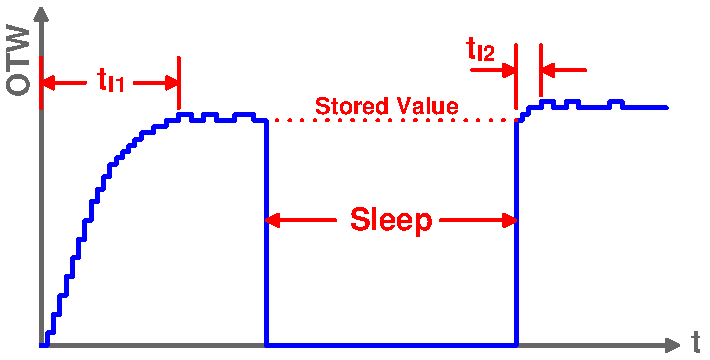
\includegraphics[width=0.6\textwidth, angle=0]{./figs/design/pll_sleep}
			    \caption{PLL sleep and resume operation.}
			    \label{fig:pll_sleep}
			\end{figure}


	\subsection{Dividerless PLL}

	\begin{figure}[htb!]
		\center\fontfamily{\sfdefault}\selectfont
% XCircuit output "bbpll_full_noise.tex" for LaTeX input from bbpll_full_noise.ps
\def\putbox#1#2#3#4{\makebox[0.00000in][l]{\makebox[#1][l]{}\raisebox{\baselineskip}[0.00000in][0.00000in]{\raisebox{#2}[0.00000in][0.00000in]{\scalebox{#3}{#4}}}}}
\def\rightbox#1{\makebox[0.00000in][r]{#1}}
\def\centbox#1{\makebox[0.00000in]{#1}}
\def\topbox#1{\raisebox{-0.60\baselineskip}[0.00000in][0.00000in]{#1}}
\def\midbox#1{\raisebox{-0.20\baselineskip}[0.00000in][0.00000in]{#1}}
   \scalebox{1}{
   \normalsize
   \parbox{5.50000in}{
   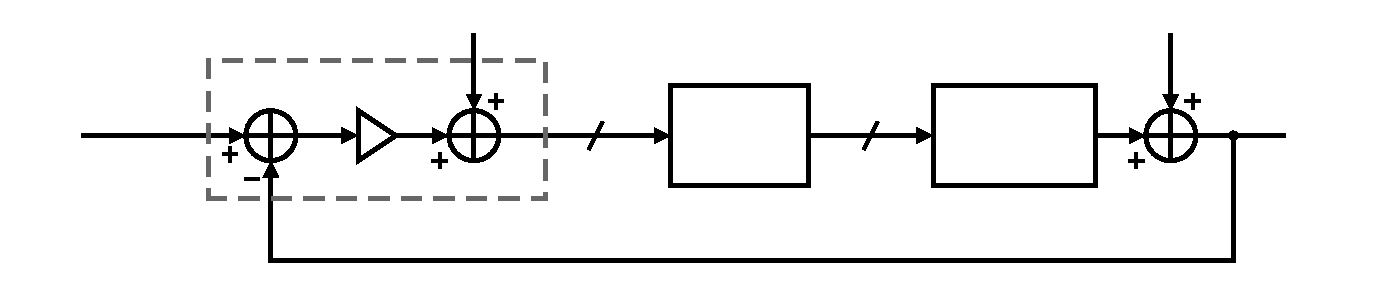
\includegraphics[scale=0.60000]{./figs/bbpll_full_noise.pdf}\\
   % translate x=416 y=448 scale 0.38
   \putbox{0.33600in}{0.70800in}{0.84}{$\Phi_{ref}$(t)}%
   \putbox{2.27400in}{0.73200in}{0.84}{e$_\Phi$(t)}%
   \putbox{1.42200in}{0.78600in}{0.84}{\rotatebox{-360}{$K_{BBPD}$}}%
   \putbox{1.20600in}{0.70800in}{0.84}{$\Phi_e$}%
   \putbox{0.83400in}{0.98400in}{0.84}{BBPD}%
   \putbox{2.77200in}{0.59400in}{0.84}{H$_{LF}$(s)}%
   \putbox{3.39600in}{0.72000in}{0.84}{u(t)}%
   \putbox{3.85800in}{0.60600in}{0.84}{$\frac{2\pi K_{DCO}}{s}$}%
   \putbox{4.82400in}{0.69600in}{0.84}{$\Phi_{out}$(t)}%
   \putbox{3.73200in}{0.87000in}{0.84}{DCO}%
   \putbox{1.93200in}{1.00800in}{0.84}{q$_{n_{BBPD}}$(t)}%
   \putbox{4.72200in}{1.00800in}{0.84}{$\Phi_{n_{DCO}}$(t)}%
   } % close 'parbox'
   } % close 'scalebox'
   \vspace{-\baselineskip} % this is not necessary, but looks better
\fontfamily{\rmdefault}\selectfont

		\caption{BBPD-PLL full noise model.}
		\label{fig:bbpll_full_noise}
	\end{figure}

	In the divider-based PLL theory (section \ref{sec:pll_output_noise}), the derived PLL detector phase noise component (equation \ref{eq:out_psd_bbpd_pll}) contains a term proportional to $N^2$, that is the detector noise will grow with the square of the PLL divider ratio. It is, however, possible to remove this $N^2$ dependency by (a) removing the divider from the PLL, and (b) using a sub-sampling phase detector \cite{Gao2015}. A subsampling phase detector operates by directly sampling the PLL output at a rate equivalent to the reference frequency. In this work, the sub-sampling phase detector is implemented in the form of a bang-bang phase detector.

	 In a dividerless PLL, it must be guaranteed that the PLL frequency at the start of sub-sampling operation be well within $f_{ref}/2$ of the target frequency (the PLL will lock to the nearest multiple of the reference frequency). In this work, although not implemented, it is suggested to implement a coarse frequency calibration scheme which can reliably tune the oscillator frequency within a small enough tolerance that the PLL can lock when BBPD-based operation is started.

	  In accordance to the change to dividerless operation, the PLL closed loop transfer function has been rederived in equation \ref{eq:cont_pll_tf2}. Furthermore, new expressions for PLL output phase noise with a BBPD is given in equation \ref{eq:out_psd_bbpd_pll2}, and PLL output oscillator noise with a ring oscillator is given in equation \ref{eq:out_psd_dco_pll2}, for the BBPD-PLL noise model in figure \ref{fig:bbpll_full_noise}. Noise due to the loop filter here is ignored, as it will be possible to adjust the loop filter datapath resolution to make digital quantization noise effects negligible.
			\begin{align} \label{eq:cont_pll_tf2}
				\mathrm{T}(s) = \frac{\Phi_{out}(s)}{\Phi_{ref}(s)} = \frac{2\pi K_{BBPD}K_{DCO}\sum_{j=0}^Z b_js^j}{\sum_{k=0}^P a_ks^{k+1} + 2\pi K_{BBPD}K_{DCO}\sum_{j=0}^Z b_js^j} = \frac{\mathrm{L}(s)}{1 + \mathrm{L}(s)}
			\end{align}
			\begin{align}\label{eq:out_psd_bbpd_pll2}
				S_{\Phi n_{BBPD,out}}(f) &= S_{n_{BBPD}}(f)\left|\frac{\Phi_{out}(f)}{q_{n_{BBPD}}(f)}\right|^2 = \frac{\left(\frac{\pi}{2}-1\right)}{f_{ref}}\left|\sigma_{\Phi_e}\mathrm{T}(f)\right|^2
			\end{align}
			\begin{align}\label{eq:out_psd_dco_pll2}
				S_{\Phi n_{DCO,out}}(f) &= \mathcal{L}_{min}(f)\left|\frac{\Phi_{out}(f)}{q_{n_{DCO}}(f)}\right|^2 = \frac{7.33k_BT}{P}\left(\frac{f_0}{f}\right)^2|1-\textnormal{T}(f)|^2 
			\end{align}

% \vspace{-2em}
% \begin{figure}[htb!]
% 	\center\fontfamily{\sfdefault}\selectfont
% XCircuit output "tdc_bbpll.tex" for LaTeX input from tdc_bbpll.ps
\def\putbox#1#2#3#4{\makebox[0.00000in][l]{\makebox[#1][l]{}\raisebox{\baselineskip}[0.00000in][0.00000in]{\raisebox{#2}[0.00000in][0.00000in]{\scalebox{#3}{#4}}}}}
\def\rightbox#1{\makebox[0.00000in][r]{#1}}
\def\centbox#1{\makebox[0.00000in]{#1}}
\def\topbox#1{\raisebox{-0.60\baselineskip}[0.00000in][0.00000in]{#1}}
\def\midbox#1{\raisebox{-0.20\baselineskip}[0.00000in][0.00000in]{#1}}
   \scalebox{1}{
   \normalsize
   \parbox{3.33750in}{
   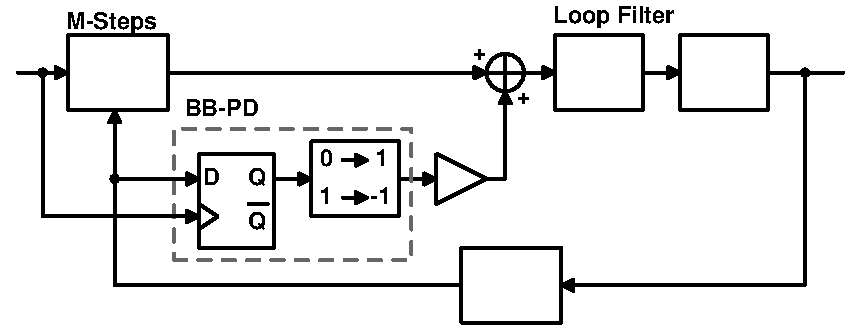
\includegraphics[scale=0.60000]{./figs/tdc_bbpll.pdf}\\
   % translate x=1412 y=528 scale 0.38
   \putbox{1.80600in}{0.70800in}{0.72}{$K_{bb}$}%
   \putbox{1.93200in}{0.14400in}{0.72}{$\div$ N}%
   \putbox{2.79600in}{0.99600in}{0.72}{DCO}%
   \putbox{2.24400in}{0.99600in}{0.72}{H$_{LF}$(z)}%
   \putbox{0.37200in}{0.99600in}{0.72}{TDC}%
   \putbox{0.03600in}{1.08600in}{0.72}{Clk}%
   \putbox{3.13200in}{1.08600in}{0.72}{Out}%
   } % close 'parbox'
   } % close 'scalebox'
   \vspace{-\baselineskip} % this is not necessary, but looks better
\fontfamily{\rmdefault}\selectfont

% 	\caption{PLL with parallel bang-bang phase detector and TDC.}
% 	\label{fig:tdc_bbpll}
% \end{figure}
	% \subsubsection{Gear Switching}
	% The proposed digital architecture enables the ability to dynamically alter the loop filter response. This can be used to speed up lock from a cold state by using a lock time optimized filter initially, and then switch to a phase noise optimized filter after achieving initial lock. This approach is called gear switching \cite{staszewski_balsara_2007}, and is employed in this work by utilizing different loop filters for the start-up synchronous counter phase detector operation and the steady state BBPD operation.
	

	\subsection{Floorplan}
	To meet the design goal to achieve state of art for implementation area, the below floor plan (dimensions in microns) has been devised such that the total area is $<<$ 0.01 mm$^2$. The final implemented dimensions are 82$\mu$m x 47$\mu$m, with an active area of 0.00365 mm$^2$.
	% The yelow path demarcates the PLL loop signal flow. Attention was paid to separate analog (0.8V) and digital power domains (0.5V), whilst maintaining a compact area with convenient signal flow.
		\begin{figure}[htb!]
	        \centering
	        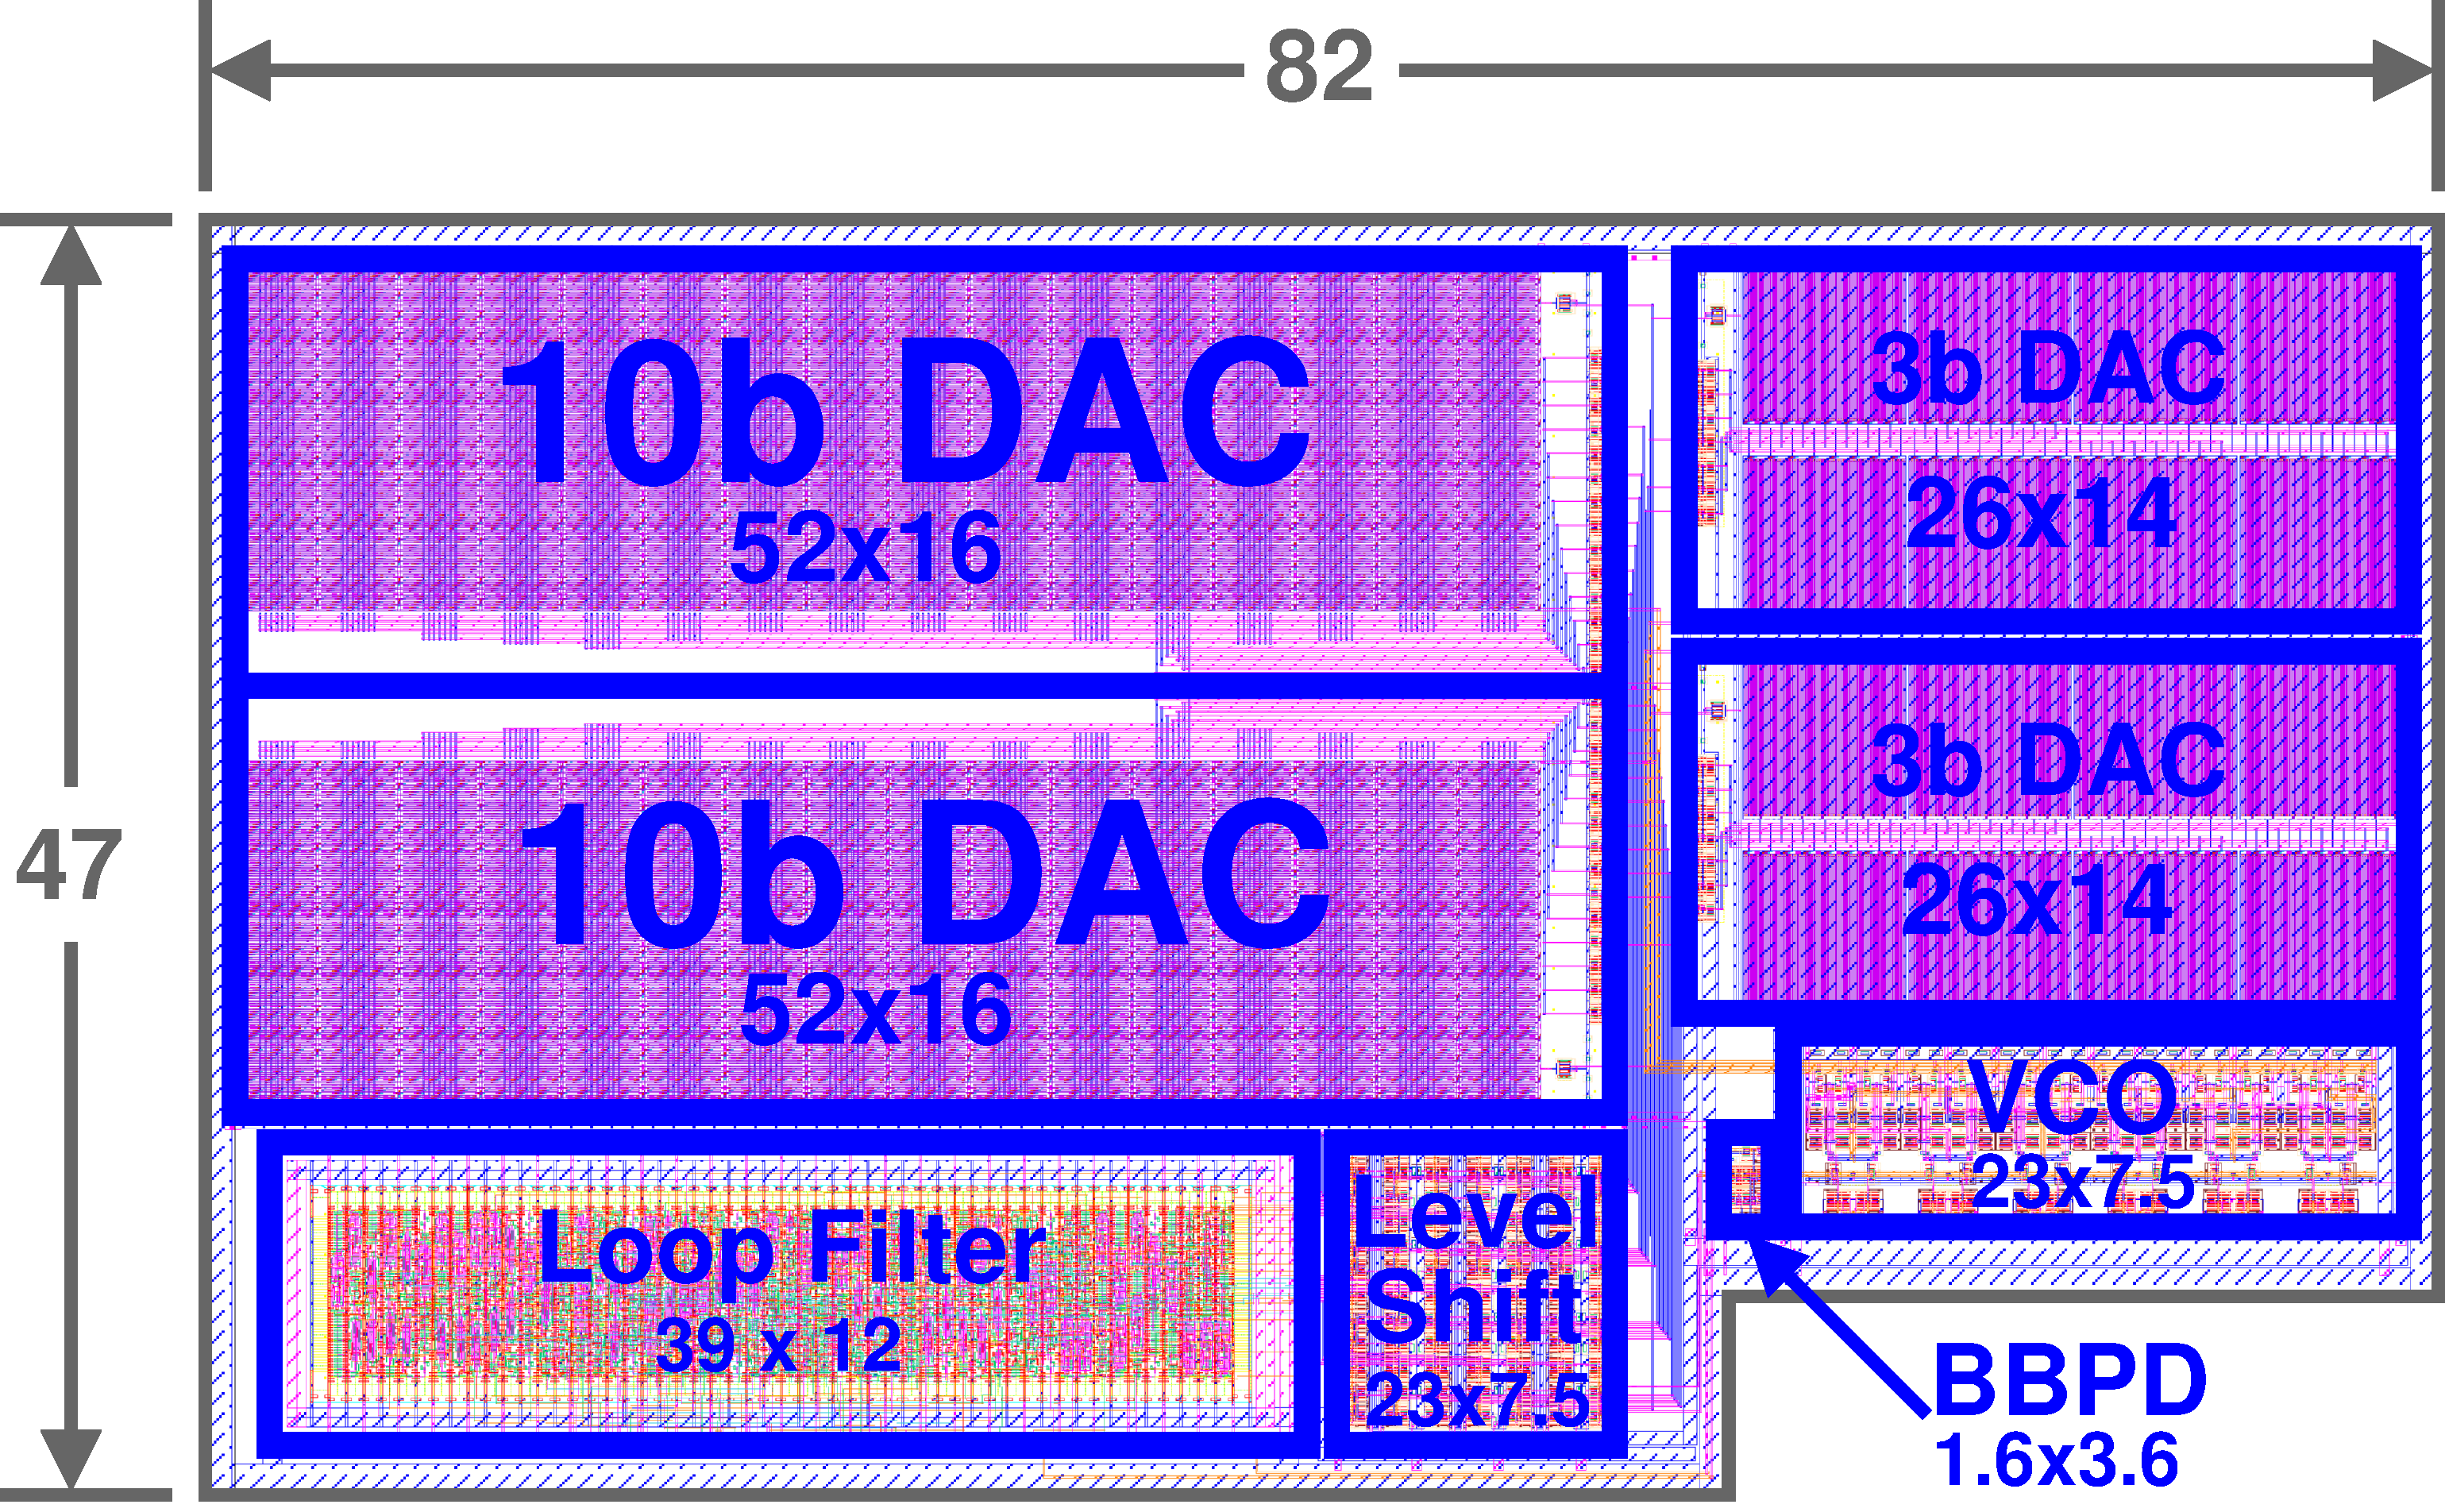
\includegraphics[width=1\textwidth, angle=0]{./figs/design/final_floorplan}
		    \caption{PLL floorplan (units in microns).}
		\end{figure}

	\subsection{Power Budget}
	The below power budget was used in the design process to divide up the 100 $\mu$W allotment between the different PLL components. In order to minimize oscillator phase noise, the portion of power for the oscillator was chosen to be as large as possible.
		\begin{table}[htb!]
			\centering
			\def\arraystretch{1.5}		
			\setlength\arrayrulewidth{0.75pt}
			\setlength{\tabcolsep}{1em} % for the horizontal padding
			\begin{tabular}{|c|c|c|c|c|}
				\hline 
				\rule[-1ex]{0pt}{2.5ex} \cellcolor{gray!40}\textbf{DCO} & \cellcolor{gray!40}\textbf{Phase detector} & \cellcolor{gray!40}\textbf{Digital (LF)}& \cellcolor{gray!40}\textbf{Other} & \cellcolor{gray!40}\textbf{SUM} \\ 
				\hline 
				\rule[-1ex]{0pt}{2.5ex} 80 $\mu$W& 5 $\mu$W &  5 $\mu$W  & 5 $ \mu$W & $\leq$ 95  $\mu$W\\ 
				\hline 
			\end{tabular} 
			\caption{Power budget for design process.}
			\label{tab:pow_budget}
		\end{table}   

	\FloatBarrier
	\subsection{Note on Reference Frequency}
	The specified reference frequency for the PLL is 32 MHz, however, with a 2.448 GHz synthesized frequency, the ratio of reference to synthesized frequency is 76.5, which implies integer-N operation is not possible. Therefore, the reference frequency must be prescaled by a factor of 2 to 16 MHz, resulting in ratio of reference to synthesized frequency of 153, an integer. The reference value of 16 MHz is used in the remainder of this work.


% ################################################################################################
% ################################################################################################
\FloatBarrier\pagebreak
\section{Phase Detector Design}\label{sec:pd_design}

		A bang-bang phase detector, as introduced in section \ref{bbpd_theory}, can be implemented physically with a D flip-flop \cite{Razavi2020} and logic to map the 0/1 valued output to a signed $\pm$1 value that may be passed into a digital loop filter. This is shown in figure \ref{fig:bbpd_dff}. 

		\begin{figure}[htb!]
			\center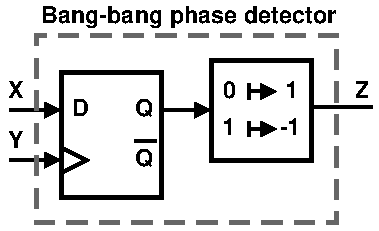
\includegraphics[width=0.4\textwidth, angle=0]{./figs/design/bbpd_}
			\caption{Bang-bang phase detector with D flip-flop.}
			\label{fig:bbpd_dff}
		\end{figure}
		The realization of a BBPD using a digital flip flop introduces additional noise to the system in the form of jitter. Jitter arises as an artifact of circuit and supply noise. For small time differentials between the BBPD inputs X and Y, the output can be stochastically corrupted due to the presence of noise. Furthermore, physical D flip flop implementations exhibit set-up and hold time requirements for data to be stable (to allow internal nodes to settle), so deterministic corruption of phase detection can be imparted if the inputs violate physical timing requirements. These sources of corruption cause BB-PD transfer characteristics in terms of output expectation, $\mathbb{E}[Z]$, with respect to input timing difference $\Delta t_{XY}$ to deviate from an ideal step response, demonstrated in figure \ref{fig:bbpd_jit_pdf}. Analytically, the corruption of the transfer characteristic can be viewed as being caused by an additive phase noise component before the signum operation in the BBPD, as shown in figure \ref{fig:bbpd_noise_nonlinear}. The expectation $\mathbb{E}[Z(\Delta t_{XY})]$ acts as a cumulative distribution function (CDF) for this phase noise component. Thus, differentiation of $\mathbb{E}[Z(\Delta t_{XY})]$ results in a probability distribution function (PDF) P(T=$\Delta t_{xy}$) of this phase noise signal. Statistical analysis of variance of the PDF provides an RMS value for timing jitter of this additive noise source, $\sqrt{\mathrm{Var}[T]} = \sigma_{t,j}$. The RMS timing jitter may be converted to RMS phase error of the noise source as $\sigma_{\Phi_j} = 2\pi f_{osc}\sigma_{t_j}$. This statistical analysis approach has been applied in this work to evaluate BBPD performance.
 
		\begin{figure}[htb!]
		    \centering
			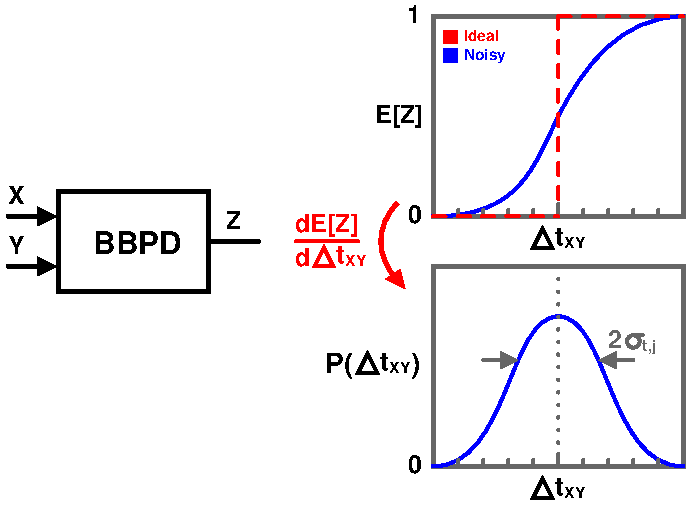
\includegraphics[width=0.6\textwidth, angle=0]{./figs/bbpd_jitter.pdf}
			\caption{BBPD output expectation and jitter PDF versus input time differential.}
			\label{fig:bbpd_jit_pdf}
		\end{figure}

	\begin{figure}[htb!]
	    \centering
	    \begin{subfigure}{0.5\textwidth}
	        \centering
	        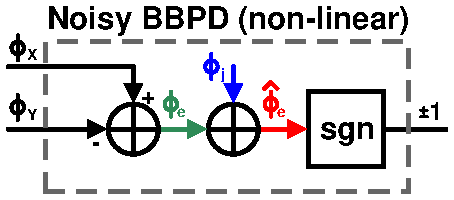
\includegraphics[width=0.8\textwidth, angle=0]{figs/design/bbpd_noise_nonlinear}
	        \caption{ }
	        \label{fig:bbpd_noise_nonlinear}
	    \end{subfigure}%
	    \begin{subfigure}{0.5\textwidth}
	        \centering
	        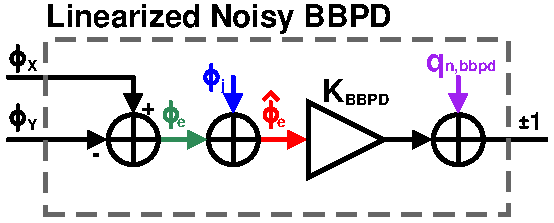
\includegraphics[width=0.9\textwidth, angle=0]{figs/design/bbpd_noise_linear}
	        \caption{ }
	        \label{fig:bbpd_noise_linear}
	    \end{subfigure}
	    % \caption{x.}
	    \caption{\textbf{(a)} Noisy BBPD nonlinear model \textbf{(b)} Noisy BBPD linearized model}
	     \label{fig:bbpd_noisy}
	\end{figure} 

	With a model including BBPD noise due to implementation non-idealities, a modified linearized model for the BBPD will be established here. This model will reconcile the ideal BBPD noise introduced in section \ref{bbpd_theory} with the noise due to the new additive jitter component just described. First, a phase noise component representing the non-ideal jitter component, $\Phi_j$, is added into the noise model from figure \ref{fig:bbpll_full_noise}. The result is the linearized model of figure \ref{fig:bbpd_noise_linear}. We then define a modified phase error, $\hat{\Phi}_e$, which includes the nominal $\Phi_e$ and the jitter corruption:
	\begin{equation}
	\hat{\Phi}_e = \Phi_e + \Phi_j.
	\end{equation}
	$\hat{\Phi}_e$ has a variance defined as $\sigma_{\hat{\Phi}_e}^2 = \sigma_{\Phi_e}^2 + \sigma_{\Phi_j}^2$, assuming $\Phi_e$ and $\Phi_j$ are uncorrelated. Defining BBPD gain in terms of $\sigma_{\hat{\Phi}_e}$, using the equation from \ref{eq:nom_bbpd_gain}:
	\begin{equation}
		K_{BBPD} = \sqrt{\frac{2}{\pi}}\cdot\frac{1}{\sigma_{\hat{\Phi}_e}} = \sqrt{\frac{2}{\pi}}\cdot\frac{1}{\sqrt{\sigma_{\Phi_e}^2 + \sigma_{\Phi_j}^2}}
	\end{equation}

	 It is then observed that the output Z is valued $\pm$1, thus its power is always $\sigma_Z^2$=1. Furthermore:
	\begin{equation}
	 	\sigma^2_{Z} = 1 = K_{BBPD}^2(\sigma^2_{\phi_e} +\sigma^2_{\phi_j})  + \sigma^2_{q_{n,BBPD}}
	\end{equation}
	 As determined in section \ref{bbpd_theory}, $\sigma^2_{q_{n,BBPD}} = 1 - \frac{2}{\pi}$. The total output noise with detector jitter is then given in equation \ref{eq:total_noise_bbpd_noise_power}.
			\begin{equation}\label{eq:total_noise_bbpd_noise_power}
				\sigma^2_{\phi_{n,BBPD}} =  \sigma^2_{q_{n,BBPD}} + K_{BBPD}^2\sigma^2_{\phi_j} =  1 - \frac{2}{\pi}\frac{\sigma^2_{\phi_e}}{\sigma^2_{\phi_j} + \sigma^2_{\phi_e}}
			\end{equation}
	If the BB-PD is connected directly to oscillator output, so $\sigma^2_{\phi_e}$ = $\sigma^2_{\phi_n}$ (i.e. the PLL output phase noise), the spectral density of the BB-PD phase noise is therefore:
		\begin{equation}
			S_{\phi_{n,BBPD}} = \frac{\sigma^2_{\phi_{n,BBPD}}}{f_{ref}} =  \frac{1 - \frac{2}{\pi}\frac{\sigma^2_{\phi_n}}{\sigma^2_{\phi_j} + \sigma^2_{\phi_n}}}{f_{ref}}
		\end{equation}

		\begin{align}\label{eq:out_psd_bbpd_pll3}
			S_{\Phi n_{BBPD,out}}(f) &= S_{n_{BBPD}}(f)\left|\frac{\Phi_{out}(f)}{q_{n_{BBPD}}(f)}\right|^2 = \frac{\frac{\pi}{2}(\sigma^2_{\phi_j} + \sigma^2_{\phi_n})-\sigma^2_{\phi_n}}{f_{ref}}\left|\mathrm{T}(f)\right|^2
		\end{align}

	% \begin{itemize}[itemsep=4pt,label=\protect---]
	% 	\item It is observed that PLL phase noise spectrum is approximately Lorentzian (except for peaking and flicker noise components). Given BB-PD noise PSD of $S_{\phi_{n,BBPD}}$, and an oscillator with noise PSD $S_{\phi_{n,osc}}(\Delta f)$, the optimal bandwidth for minimum noise power is:

	% 	\begin{equation}
	% 		BW_{opt} =  \sqrt{\frac{S_{\phi_{n,osc}}(\Delta f)}{S_{\phi_{n,BBPD}}}}\Delta f
	% 	\end{equation}
	% 	\item The total PLL output phase noise with optimal bandwidth is then:

	% 	\begin{equation}
	% 		\sigma^2_{\phi_{n,opt}} =   \pi\sqrt{\phi_{n,osc}(\Delta f)S_{\phi_{n,BBPD}}}\Delta f
	% 	\end{equation}
	% \end{itemize}
	% \vspace{-3em}
	% \begin{figure}[htb!]
	%     \centering
	%     \begin{subfigure}{0.33\textwidth}
	%         \centering
	%         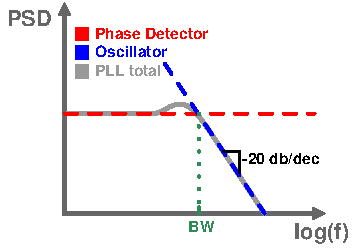
\includegraphics[width=1\textwidth, angle=0]{./figs/pll_spectrum_lorentzian.pdf}
	%     \end{subfigure}%
	%     \begin{subfigure}{0.33\textwidth}
	%         \centering
	%         \center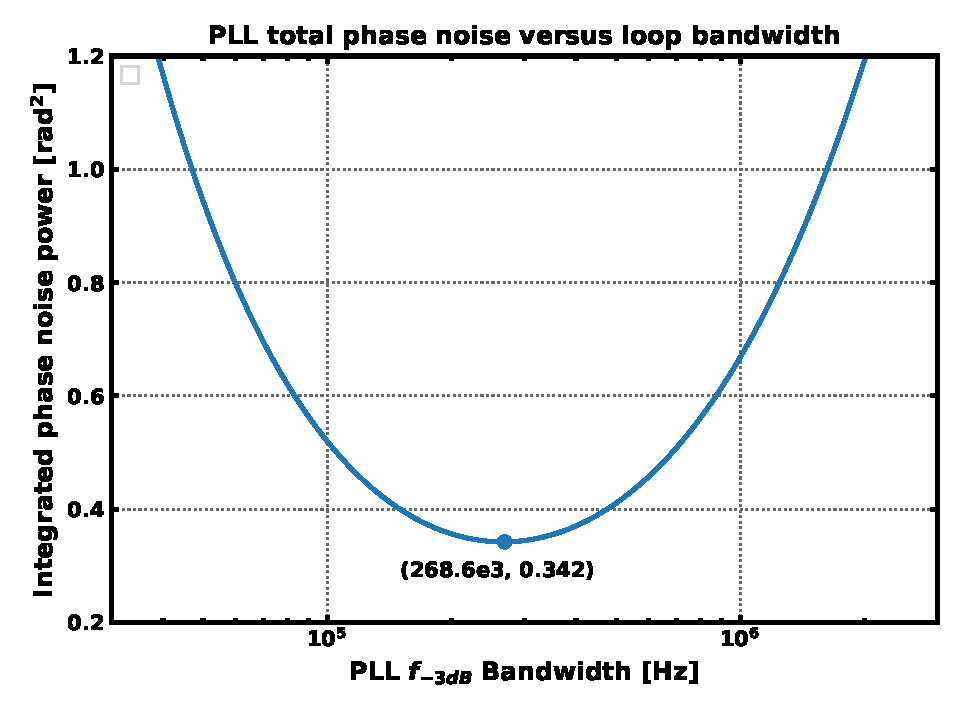
\includegraphics[width=1.0\textwidth, angle=0]{./figs/bandwidth_vs_pn.pdf}
	%     \end{subfigure}
	%     % \caption{Approximate model for ring oscillator inverter delay cell.}
	% \end{figure}




	% \begin{itemize}[itemsep=4pt,label=\protect---]
	% 	\item Using the findings for BB-PD noise PSD, assumption of Lorentzian spectrum, and constraint that BW = $\alpha f_{ref}$ (recommended $\alpha$$<$0.1 [2], rule of thumb since ancient PLL days). Given oscillator center frequency $f_c$, BB-PD jitter is constrained:

	% 	\begin{equation}
	% 		\sigma_{t_j} \leq \frac{\sigma_{\Phi_n}}{2\pi f_c}\sqrt{\frac{2}{\pi}\left(\frac{1}{\pi\alpha} - \frac{\pi}{2} + 1\right)} = \frac{\sigma_{\Phi_n}}{2\pi f_c}\beta(\alpha)
	% 	\end{equation}
	% 	\item $\beta(\alpha=0.1)$ = 1.28, $\beta(\alpha=0.05)$ = 1.92.
	% 	\item Using my PLL specifications ($f_c$ = 2.448 GHz, CNR = -$\sigma_{\Phi_n}$ = 17 dB, $\alpha=0.1$), {\color{red}\textbf{$\sigma_{t,j}\leq 11.8 $ ps}}
	% \end{itemize}



	% \begin{itemize}[itemsep=4pt,label=\protect---]
	% 	\item With an unconstrained relationship for BW and $f_{ref}$, and the optimal bandwidth finding, it is determined that the optimal value of $\sigma_{t,j}$ for minimum phase noise is:

	% 	\begin{equation}
	% 		\sigma_{t_j,opt} = \frac{\sigma_{\Phi_n}}{2\pi f_c}\sqrt{\frac{2}{\pi}\left[\frac{\sigma^4_{\Phi_n} f_{ref}}{\pi^2 S_{\phi_{n,osc}}(\Delta f) \Delta f^2} - \left(\frac{\pi}{2} - 1\right)\sigma^2_{\Phi_n}\right]}
	% 	\end{equation}

	% \end{itemize}

	% \begin{itemize}[itemsep=4pt,label=\protect---]
	% 	\item Setting the two jitter equations of the last side equal, it is found that optimal phase noise power is:

	% 	\begin{equation}
	% 		\sigma^2_{\Phi_n, opt} = \frac{\pi S_{\phi_{n,osc}}(\Delta f) \Delta f^2}{\alpha f_{ref}}
	% 	\end{equation}
	% 	\item The optimal reference frequency ($\sigma_{\Phi_n}=2\pi f_c \sigma_{t_n}$ = CNR):
	% 	\begin{equation}
	% 		f_{ref} = \frac{\pi S_{\phi_{n,osc}}(\Delta f) \Delta f^2}{\alpha \sigma^2_{\Phi_n}}
	% 	\end{equation}
	% 	\item The optimal oscillator phase noise at offset $\Delta f$:
	% 	\begin{equation}
	% 		S_{\phi_{n,osc}}(\Delta f) = \frac{\alpha f_{ref}\sigma^2_{\Phi_n}}{\pi \Delta f^2} 
	% 	\end{equation}
	% 	\item For CNR = 17 dB, $S_{\phi_{n,osc}}(\Delta f = 1 MHz)$ = -80 dBc/Hz, $\alpha$ = 0.1, {\color{red}the optimal $f_{ref}$ = 15.7 MHz.}
	% 	\item For CNR = 20 dB, $S_{\phi_{n,osc}}(\Delta f = 1 MHz)$ = -80 dBc/Hz, $\alpha$ = 0.1, {\color{red}the optimal $f_{ref}$ = 31.4 MHz.}
	% \end{itemize}


		\FloatBarrier






		\subsection{Circuit}
		The physical implementation of the bang-bang phase detector has been selected to utilize a true single phase clock (TSPC) D flip-flop \cite{Yuan1989}. The positive-edge triggered variant of this circuit has been implemented as shown in figure \ref{fig:tspc_dff}. Selection of this topology was based on the desire for the usage of a single ended clock as a reference signal.

			\begin{figure}[htb!]
			        \centering
			        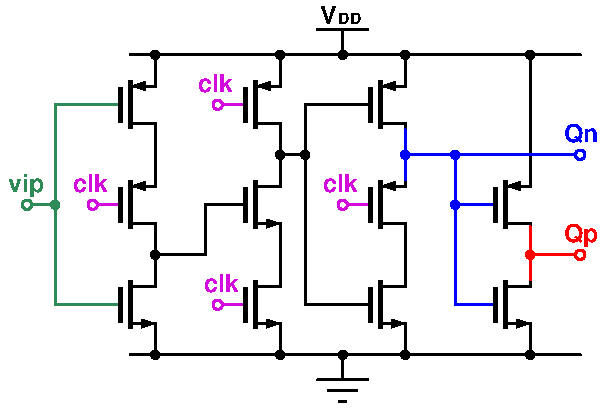
\includegraphics[width=0.55\textwidth, angle=0]{./figs/design/tspc_}
			    \caption{True single-phase clock (TSPC) D flip-flop, positive edge triggered.}
			    \label{fig:tspc_dff}
			\end{figure}

		This TSPC design was validated in simulation with regular voltage threshold (RVT) devices in the 22nm FD-SOI process with all devices set to have equal (W/L). (W/L) $\in$ \{100n/20n, 200n/20n\} were tested, and supply voltages of 0.5 and 0.8 volts were tested. It was determined that the implementation with (W/L) = 200n/20n for all devices and $V_{DD}$ = 0.8 was satisfactory, as a low jitter value of 1.342 ps with 0.46 $\mu$W of power consumption was found, far lower than the 5 $\mu$W limit set in the power budget. The excess power allotment not used by the BBPD in the original power budget has been reassigned to the oscillator. Final simulation results for the BBPD are in the results section \ref{sec:res_bbpd}, and the layout in appendix \ref{sec:lay_bbpd}.


		% \end{itemize}
		% % \vspace{-3em}
		% \begin{figure}[htb!]
		%     \centering
		%     \begin{subfigure}{0.5\textwidth}
		%         \centering
		%         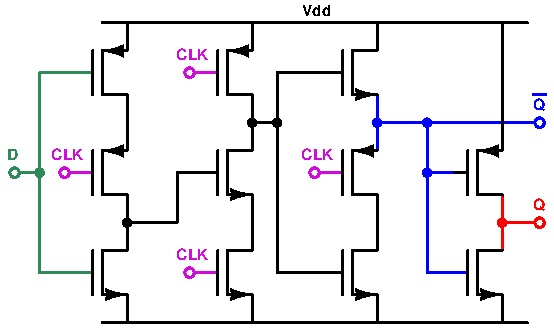
\includegraphics[width=0.8\textwidth, angle=0]{./figs/tspc_dff.pdf}
		%         \caption{TSPC DFF}
		%     \end{subfigure}%
		%     \begin{subfigure}{0.5\textwidth}
		%         \centering
		%         \center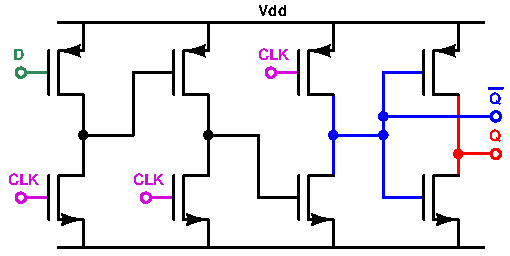
\includegraphics[width=0.8\textwidth, angle=0]{./figs/etspc_dff.pdf}
		%         \caption{e-TSPC DFF}
		%     \end{subfigure}
		%     % \caption{Approximate model for ring oscillator inverter delay cell.}
		% \end{figure}


	% \begin{itemize}[itemsep=4pt,label=\protect---]
	% 	\item Utilized TSPC DFF, with inverter buffers (FETs sized 200n/20n) for clock and data buffers.
	% 	\item Sweep delay between inputs, calculating the expect value of the output for 100 bits. Transient noise simulated (up to 100 GHz), and the inital state of the FF is set to be high 50x and low 50x to include hysteresis effects. 
	% 	\item V$_{DD} \in$ \{0.5, 0.8\} V and (W/L) $\in$ \{100n/20n, 200n/20n\} tested. 100 aF added to every node.
	% 	\item \textbf{Resulting CDFs of the input time delta versus output expectation are below.}
	% \end{itemize}
	% \vspace{-2em}
	% \begin{figure}[htb!]
	%     \centering
	% 	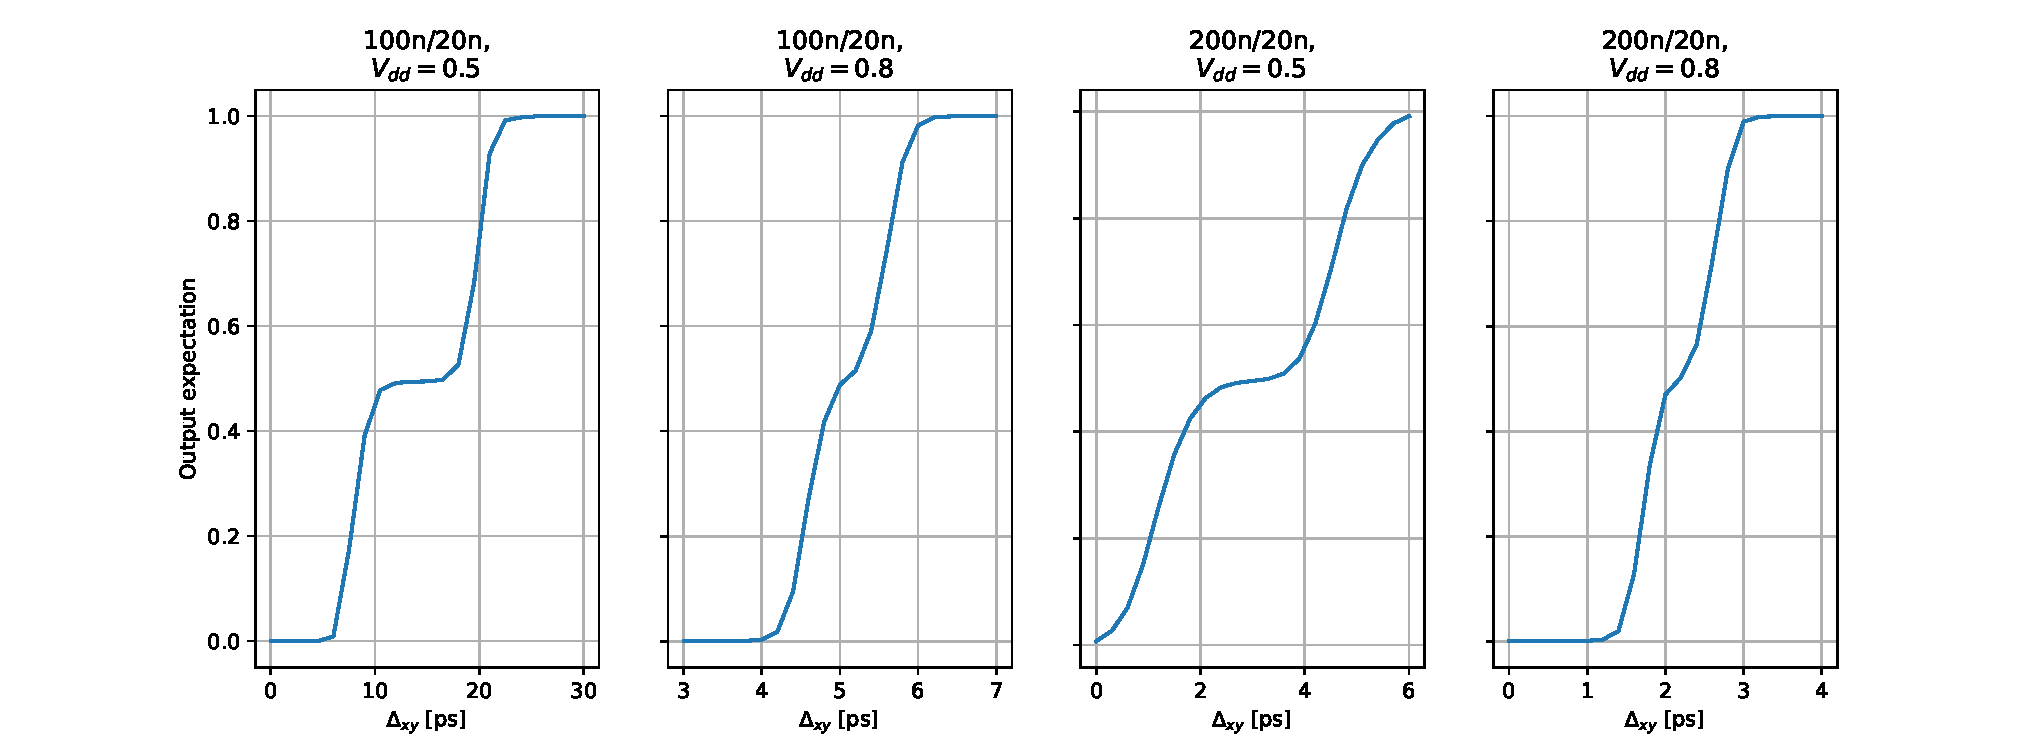
\includegraphics[width=1\textwidth, angle=0]{./figs/cdfs.pdf}
	% \end{figure}

	% \begin{itemize}[itemsep=4pt,label=\protect---]
	% 	\item Jitter PDFs are bimodal from hysteresis of DFF. 
	% 	\item Increasing (W/L) or $V_{DD}$ both impact jitter favorably.
	% 	\item \textbf{The jitter PDF (computed from the CDFs) of the input time delta versus output expectation are below. (Delays are removed)}
	% \end{itemize}
	% \vspace{-2em}
	% \begin{figure}[htb!]
	%     \centering
	% 	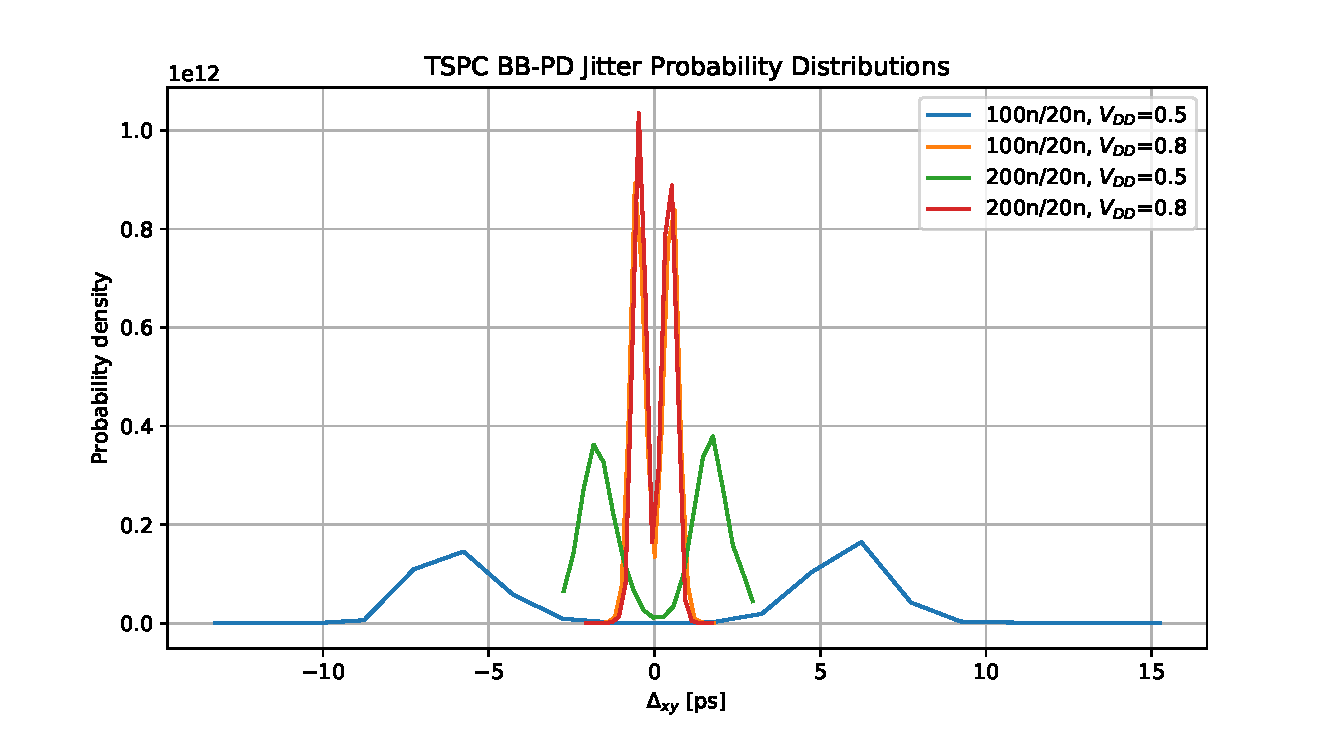
\includegraphics[width=0.7\textwidth, angle=0]{./figs/jitter_pdfs.pdf}
	% 	\caption{Jitter PDF from simulated TSPC DFFs.}
	% 	\label{fig:tspc_dff_sim}
	% \end{figure}


		% \begin{table}[h!]
		% 	\centering
		% 	\def\arraystretch{1.5}		
		% 	\setlength\arrayrulewidth{0.75pt}
		% 	\setlength{\tabcolsep}{1em} % for the horizontal padding
		% 	\begin{tabular}{|c|c|c|c|}
		% 		\hline 
		% 		\rule[-1ex]{0pt}{2.5ex} \cellcolor{gray!40}\textbf{(W/L)} & \cellcolor{gray!40}\textbf{Supply [V]} & \cellcolor{gray!40}\textbf{RMS jitter [ps]}& \cellcolor{gray!40}\textbf{Power [$\mu$W]}\\ 
		% 		\hline 
		% 		\rule[-1ex]{0pt}{2.5ex} 100n/20n  & 0.5 & 6.01 & 1.64\\ 
		% 		\hline 
		% 		\rule[-1ex]{0pt}{2.5ex} 100n/20n  & 0.8 & 0.832  & 3.942\\ 
		% 		\hline 
		% 		\rule[-1ex]{0pt}{2.5ex} 200n/20n  & 0.5 & 1.776 & 2.215 \\ 
		% 		\hline 
		% 		\rule[-1ex]{0pt}{2.5ex} 200n/20n  & 0.8 & 0.496  & 4.591 \\ 
		% 		\hline 
		% 	\end{tabular} 
		% 	\caption{Schematic simulation of TSPC DFF.}
		% 	\label{tab:dff}
		% \end{table}   
		% \FloatBarrier{\color{white}.}







		% \FloatBarrier
		% \subsubsection{Layout}
		% 	\hl{Area?}
		% 	\begin{figure}[htb!]
		% 	        \centering
		% 	        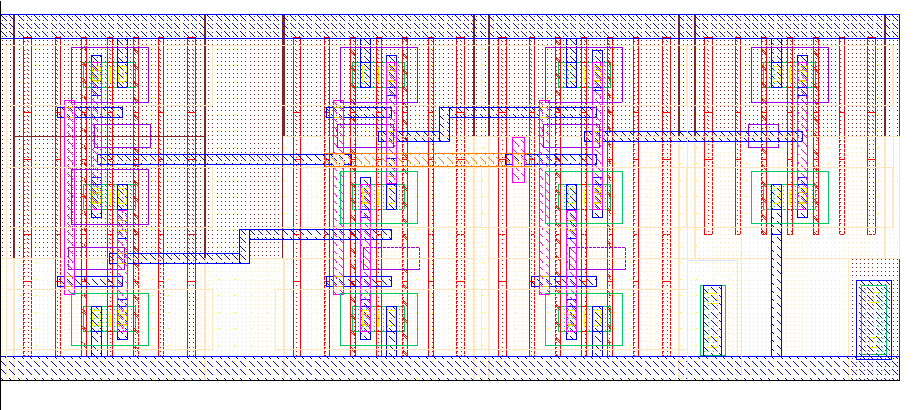
\includegraphics[width=\textwidth, angle=0]{./figs/layout/layout_bbpd}
		% 	    \caption{Single ended bang-bang phase detector.}
		% 	\end{figure}





% ################################################################################################
% ################################################################################################
\FloatBarrier\pagebreak
\section{Loop Filter Design}\label{sec:design_lf}
	% \pagebreak\FloatBarrier
	% \subsection{Loop Filter}
	For selection of the loop filter topology, some basic criteria have been selected for desirable synthesizer behavior:
	\begin{enumerate}[itemsep=0pt,label=\protect\mycirc{\arabic*}]
		\setlength\itemsep{-0.8em}
		\item Zero steady state error, for accuracy of the synthesized frequency.
		\item Minimize complexity of implemented logic (i.e. minimize the number of loop filter poles and zeros).
		\item Low pass response of PLL in closed-loop.
	\end{enumerate}
	From the author of this work's previous findings \cite{Me}, it was established that the pole-zero filter that best satisfies these requirements is a proportional-integral controller.

\subsection{Proportional-integral Controller Loop Filter}
 A proportional-integral controller \cite{ogata_2010_pid} is given in equation \ref{eq:pi_pll_tf}, containing an proportional gain term $K_p$, and an integral gain term $K_i$. This can be optionally represented using a pole at zero frequency and a zero at frequency $\omega_z = K_i/K_p$.
			\begin{equation} \label{eq:pi_pll_tf}
				\textnormal{H}_{LF}(s) = K_p + \frac{K_i}{s}  = \frac{K_i}{s}\left(\frac{s}{\omega_z} + 1\right) 
			\end{equation}
			Substitution of this controller into the PLL closed loop transfer function (equation \ref{eq:cont_pll_tf2}) results in equation \ref{eq:pi_bbpdpll_tf}.
			\begin{equation}\label{eq:pi_bbpdpll_tf}
				T(s) = \frac{\Phi_{out}(s)}{\Phi_{ref}(s)} =  \frac{ 2\pi K_{BBPD}K_{DCO}K_{i} \left(\frac{s}{\omega_z} + 1\right) }{s^2 + 2\pi K_{BBPD}K_{DCO}K_{i}\left(\frac{s}{\omega_z} + 1\right) }
			\end{equation}

	\subsection{Discretization of the Loop Filter}\label{disc_lf_comp_pi}
		Using the continuous filter discretization approach described in section \ref{lf-discretization} on the loop filter of equation \ref{eq:pi_pll_tf} results in equation \ref{eq:z_lf}. When converting a continuous time PLL model into a discrete time controller implementation, a commonly cited rule of thumb in PLL literature states that the PLL loop bandwidth should be constrained as $BW_{loop} \leq$  0.1$f_{ref}$ \cite{gardner_1980} (here $\Delta T_s = 1/f_{ref}$). This is due to the fact that low degrees of oversampling lead to deviations between continuous PLL models and real sampled-PLL performance, possibly causing instability or sub-optimal performance versus an intended design.
		\begin{align}
			\textnormal{H}_{LF}(z) & = \left.\frac{K_i}{s}\left(\frac{s}{\omega_z} + 1\right)\right\vert_{s=\frac{1}{\Delta T_s}(1-z^{-1})}
			&= K_p\frac{(1+\omega_z\Delta T_s)-z^{-1}}{1- z^{-2}}\label{eq:z_lf}
		\end{align}

		The transformation of equation \ref{eq:z_lf} into a digitally implementable design as a direct form 1 IIR filter shown in figure \ref{fig:filt_imple}. Its filter coefficients are given by equations \ref{eq:b0_coef} and \ref{eq:b1_coef}.
		\begin{figure}[htb!]
			\center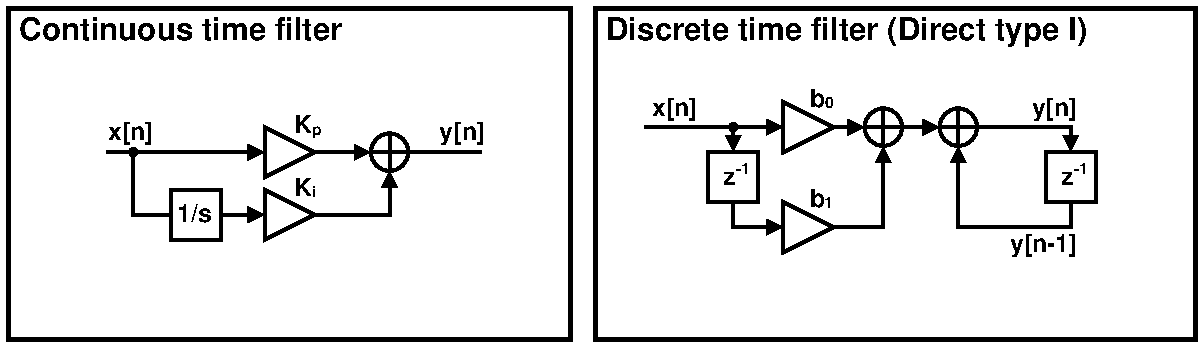
\includegraphics[width=1\textwidth, angle=0]{./figs/design/filter_arch_pi}
			\caption{Implementation of filter.}
			\label{fig:filt_imple}
		\end{figure}

		\begin{align}
			b_0 &= K_p (1+\omega_z\Delta T_s) \label{eq:b0_coef}\\
			 b_1 &= -K_p \label{eq:b1_coef}
		\end{align}

\subsection{Filter Simplification}\label{sec:filter_simplification}
			 In order to aid later optimization of the loop filter, some mathematical simplifications of the PLL model are introduced here to the PI-filter design of equation \ref{eq:pi_bbpdpll_tf}. Rewriting equation \ref{eq:pi_bbpdpll_tf} with substitutions $\omega_z = K_i/K_p$ and the gain constant $\mathrm{K} = 2\pi K_{BBPD}K_{DCO}K_{i}$:
			\begin{equation} \label{eq:simp_pi_pll_tf}
				T(s) = \frac{\Phi_{out}(s)}{\Phi_{ref}(s)} = \frac{s\frac{K}{\omega_z} + K }{s^2 + s\frac{K}{\omega_z} + K}
			\end{equation}
			The denominator can be redefined in terms of a natural frequency $\omega_n$ and damping ratio $\zeta$:
			\begin{equation}
				s^2 + s\frac{K}{\omega_z} + K = s^2 + s2\zeta\omega_n + \omega_n^2
			\end{equation}
			Thus, $\omega_n = \sqrt{K}$, and $\omega_z = \sqrt{K}/2\zeta$. The poles of equation \ref{eq:simp_pi_pll_tf} are then located at s = $\zeta\sqrt{K} \pm j\sqrt{K}\sqrt{1-\zeta^2}$. The time constant of the PLL is obtained from the real portion of the dominant pole in equation \ref{eq:simp_pi_pll_tf}:
			\begin{equation}
				\tau = \frac{1}{|\min(\Re(\{s_{p1}, s_{p2}\}))|}
			\end{equation}
			 It is of interest to minimize settling time of the PLL (i.e. time constant), thus maximizing the frequency of the dominant pole of the PLL is of interest. In the pole-zero plot of figure \ref{fig:pi_pll_pz}, the dominant pole of equation \ref{eq:simp_pi_pll_tf} is observed to be maximized with $\zeta=1$ (loci are oriented based on increasing $\zeta$ values). Typically $\zeta$ is constrained in the range of $\sqrt{2}/2$ or 1 \cite{razavi_2017}, to avoid excessive ringing. Accordingly it has been chosen to fix $\zeta=1$ for the PI-controller.

			\begin{figure}[htb!]
				\center\fontfamily{\sfdefault}\selectfont
% XCircuit output "pi_pz_plot.tex" for LaTeX input from pi_pz_plot.ps
\def\putbox#1#2#3#4{\makebox[0.00000in][l]{\makebox[#1][l]{}\raisebox{\baselineskip}[0.00000in][0.00000in]{\raisebox{#2}[0.00000in][0.00000in]{\scalebox{#3}{#4}}}}}
\def\rightbox#1{\makebox[0.00000in][r]{#1}}
\def\centbox#1{\makebox[0.00000in]{#1}}
\def\topbox#1{\raisebox{-0.60\baselineskip}[0.00000in][0.00000in]{#1}}
\def\midbox#1{\raisebox{-0.20\baselineskip}[0.00000in][0.00000in]{#1}}
   \scalebox{1}{
   \normalsize
   \parbox{4.20000in}{
   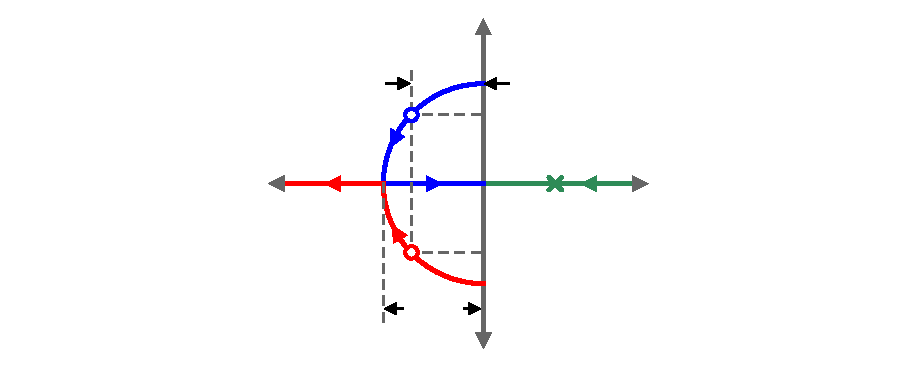
\includegraphics[scale=0.70000]{./figs/pi_pz_plot.pdf}\\
   % translate x=800 y=416 scale 0.38
   \putbox{2.85600in}{0.67900in}{1.20}{$\Re(s)$}%
   \putbox{2.30300in}{1.52600in}{1.20}{$\Im(s)$}%
   \putbox{1.89000in}{0.21700in}{1.20}{$\sqrt{\mathrm{K}}$}%
   \putbox{1.45600in}{1.36500in}{1.20}{$\zeta\sqrt{\mathrm{K}}$}%
   \putbox{2.38700in}{0.95900in}{1.20}{$\sqrt{\mathrm{K}}/2\zeta$}%
   } % close 'parbox'
   } % close 'scalebox'
   \vspace{-\baselineskip} % this is not necessary, but looks better
\fontfamily{\rmdefault}\selectfont

				\caption{PI-controller PLL pole-zero locations.}
				\label{fig:pi_pll_pz}
			\end{figure}
			\FloatBarrier
			% To illustrate the effect of the damping ratio $\zeta$, figure \ref{fig:pi_pll_response} illustratesexample frequency and step responses of a PI-controlled PLL. It is observed that increasing ringing and peaking is obtained with increasing values of $\zeta$. This is undesirable from a stability standpoint, and increased peaking in the PLL transfer function will increase output phase noise contributions, also undesirable. Therefore, the selection of $\zeta=1$ is solidified.
			% \begin{figure}[htb!]
			% 	\center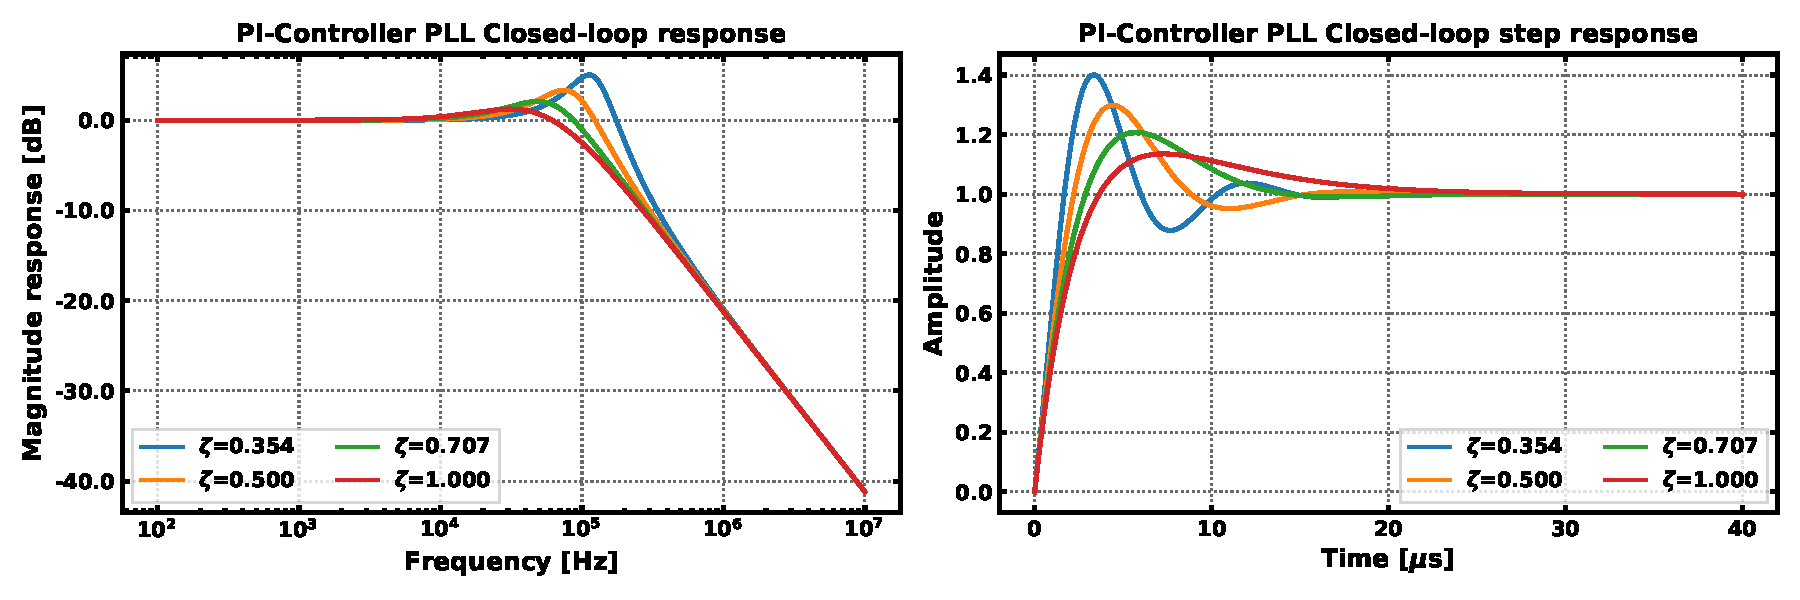
\includegraphics[width=1.0\textwidth, angle=0]{figs/pi_pll_response.pdf}
			% 	\caption{Example PI-PLL responses with varied $\zeta$.}
			% 	\label{fig:pi_pll_response}
			% \end{figure}
			% \FloatBarrier
			With $\zeta$ is constrained to 1, the final simplified PLL closed loop transfer function is in equation \ref{eq:simp_pi_pll_tf_z1}. The form of this equation is favorable for computing integrations, allowing for a closed form solution to be found for the different PLL phase noise contributions. Furthermore, this transfer function only contains one parameter, $K$, which allows for simple single-variate optimization to be undertaken for the filter design.
			\begin{equation} \label{eq:simp_pi_pll_tf_z1}
				T(s) = \frac{2\sqrt{K}s + K }{s^2 + 2\sqrt{K}s + K}
			\end{equation}
			



			\subsection{Filter Optimization (Noisy BBPD)}\label{sec:opt_lf_noisy_bbpd}	
			Optimization of a loop filter under BBPD operation will be performed by minimizing the total integrated phase noise power out of the PLL. Accordingly, the PLL output referred noise power of the oscillator and BBPD will be calculated. First, the phase noise density of the oscillator (without the PLL) is defined as equation \ref{eq:osc_spectrum}, where $S_{0_{osc}}$ is defined as the oscillator spectral density at 1 Hz frequency offset from the carrier. This is in the same form as the theoretical limit for ring oscillator phase noise in section \ref{sec:ro_pn_limit}. $S_{0_{osc}}$ can be found from a phase noise measurement of the oscillator $\mathcal{L}(f)$ at carrier offset $f$.
			% For the purposes of this work, T = 300K, $f_{osc}$ = 2.448 GHz, $P_{DC}$ = 80$\mu$W, resulting in a minimum value of $S_{0_{osc},min}$ = 2274 rad$^2$/Hz. 
			\begin{equation}\label{eq:osc_spectrum} 
				\mathcal{L}(f) = \frac{S_{0_{osc}}}{f^2} \hspace{1em}\rightarrow \hspace{1em} S_{0_{osc}} = \mathcal{L}(f)f^2
			\end{equation} 
			% \begin{equation}\label{eq:min_norm_osc_psd} 
			% 	S_{0_{osc},min} = \left.\mathcal{L}_{min}(f)f^2\right|_{f=1} = \frac{7.33 k_B T f_{osc}^2}{P_{DC}} \hspace{1em}\textnormal{rad}^2/\textnormal{Hz}
			% \end{equation}
			The PLL output spectrum is then computed as: 
			\begin{align}\label{eq:out_psd_dco_pll3} 
				S_{\Phi n_{DCO,out}}(f) &= \mathcal{L}(f)|1-\textnormal{T}(f)|^2  =  \frac{S_{0_{osc}}}{f^2}|1-\textnormal{T}(f)|^2  
			\end{align} Now, $|1-\textnormal{T}(f)|^2$ is found to be after much simplification:
			\begin{equation} |1-\textnormal{T}(f)|^2 =
				\frac{f^4}{\left(f^2+\frac{K}{(2\pi)^2}\right)^2} 
			\end{equation} 

			Thus, re-evaluating equation \ref{eq:out_psd_dco_pll3} yields:
			\begin{align}\label{eq:out_psd_dco_pll4} 
				S_{\Phi n_{DCO,out}}(f) &= S_{0_{osc}}\frac{f^2}{\left(f^2+\frac{K}{(2\pi)^2}\right)^2} 
			\end{align} 

			The total PLL phase noise power associated with the oscillator, $\sigma_{\Phi_{n,DCO}}^2$ is achieved by integrating equation \ref{eq:out_psd_dco_pll4} with respect to frequency.
			\begin{align}\label{eq:out_psd_dco_pll5} 
				\sigma_{\Phi_{n,DCO}}^2 =
				\int_{-\infty}^{\infty} S_{\Phi n_{DCO,out}}(f)df &=
				S_{0_{osc}}\int_{-\infty}^{\infty}\frac{f^2}{\left(f^2+\frac{K}{(2\pi)^2}\right)^2}df
				\\ &= S_{0_{osc}}\frac{\pi^2}{\sqrt{K}} 
			\end{align} 

			Next, the total BBPD noise at the PLL output is computed. The expression for BBPD noise density in equation \ref{eq:out_psd_bbpd_pll3} will be used, and for which $|\textnormal{T}(f)|^2$ must be computed. This is: 
			\begin{equation} 
				|\textnormal{T}(f)|^2 =
				\frac{4\frac{K}{(2\pi)^2}f^2 +
				\frac{K^2}{(2\pi)^4}}{\left(f^2+\frac{K}{(2\pi)^2}\right)^2} 
			\end{equation}

			The resulting BBPD spectral density equation is:
			\begin{align}\label{eq:out_psd_bbpd_pll4} 
				S_{\Phi n_{BBPD,out}}(f) & =
				\frac{\frac{\pi}{2}(\sigma^2_{\phi_j} +
				\sigma^2_{\phi_n})-\sigma^2_{\phi_n}}{f_{ref}}\left|\mathrm{T}(f)\right|^2
				\\&= \frac{\frac{\pi}{2}(\sigma^2_{\phi_j} +
				\sigma^2_{\phi_n})-\sigma^2_{\phi_n}}{f_{ref}}\cdot\frac{4\frac{K}{(2\pi)^2}f^2
				+ \frac{K^2}{(2\pi)^4}}{\left(f^2+\frac{K}{(2\pi)^2}\right)^2} 
			\end{align} 

			The total PLL phase noise power associated with the BBPD, $\sigma_{\Phi_{n,BBPD}}^2$ is achieved by integrating equation \ref{eq:out_psd_bbpd_pll4} with respect to frequency:
			\begin{align}\label{eq:out_psd_bbpd_pll5} 
				\sigma_{\Phi_{n,BBPD}}^2 & =
				\frac{\frac{\pi}{2}(\sigma^2_{\phi_j} +
				\sigma^2_{\phi_n})-\sigma^2_{\phi_n}}{f_{ref}}\int_{-\infty}^{\infty}\frac{4\frac{K}{(2\pi)^2}f^2
				+ \frac{K^2}{(2\pi)^4}}{\left(f^2+\frac{K}{(2\pi)^2}\right)^2}df\\ 
				&= \frac{5\sqrt{K}}{4f_{ref}}\cdot\left[\frac{\pi}{2}(\sigma^2_{\phi_j} +
				\sigma^2_{\phi_n})-\sigma^2_{\phi_n}\right] 
			\end{align} 

			The total phase noise power out of the PLL is therefore the sum of $\sigma_{\Phi_{n,BBPD}}^2$ and $\sigma_{\Phi_{n,DCO}}^2$ : 
			\begin{align} \label{eq:total_pll_pn_pow}
				\sigma^2_{\phi_n}  = \sigma_{\Phi_{n,DCO}}^2 + \sigma_{\Phi_{n,BBPD}}^2 =
				S_{0_{osc}}\frac{\pi^2}{\sqrt{K}} +
				\frac{5\sqrt{K}}{4f_{ref}}\cdot\left[\frac{\pi}{2}(\sigma^2_{\phi_j} +
				\sigma^2_{\phi_n})-\sigma^2_{\phi_n}\right] 
			\end{align} 
			Reorganization of equation \ref{eq:total_pll_pn_pow} in terms of $\sigma^2_{\phi_n}$ yields:
			\begin{align} \label{eq:total_pll_pn_pow2} \sigma^2_{\phi_n}  =
				\frac{S_{0_{osc}}\frac{\pi^2}{\sqrt{K}} +
				\frac{5\pi\sqrt{K}}{8f_{ref}}\sigma^2_{\phi_j}}{1-\frac{5\sqrt{K}}{4f_{ref}}(\frac{\pi}{2}-1)}
			\end{align}			 

			% In the special case of an ideal BBPD where $\sigma^2_{\phi_j}$ = 0, the optimal value of $K$ that minimizes total phase noise can be determined by solving for $d\sigma^2_{\phi_n}/dK = 0$, yielding:
			% \begin{align} \label{eq:k_opt} K_{opt} =
			% 	\left(\frac{4}{5}\cdot\frac{f_{ref}}{\pi-2}\right)^2 
			% \end{align}	 

			% The corresponding optimal value of $\sigma^2_{\phi_n} $ is in equation \ref{eq:total_pll_pn_pow_opt}. This should be the absolute best case achievable with a BBPD PLL with a PI-controller. For this design, with 80$\mu$W oscillator power at 2.448 GHz, 16 MHz reference, and 300K ambient temperature, the theoretical best attainable phase noise is $\sigma^2_{\phi_{n,opt}}=0.004$, or a CNR of 24 dB, above the desired 20 dB. Therefore, the current design targets are feasible under ideal circumstances. 
			% \begin{align} \label{eq:total_pll_pn_pow_opt} 
			% 	\sigma^2_{\phi_{n,opt}}  =
			% 	\frac{5\pi^2S_{0_{osc}}}{f_{ref}}\left(\frac{\pi}{2}-1\right) 
			% \end{align}	 

			In the presence of a non-ideal phase detector having phase noise power $\sigma^2_{\phi_j} = (2\pi f_{osc})^2\sigma^2_{t_j}$, where $\sigma_{t_j}$ is the detector's jitter in time, the optimal value K that minimizes phase noise is obtained as the solution of $d\sigma^2_{\phi_n}/dK = 0$. This result is given in equation \ref{eq:noisy_opt_k}. The obtained result for $K_{opt}$ may be substituted into equation \ref{eq:total_pll_pn_pow2} to determine the total noise power $\sigma^2_{\phi_n}$. 
			\begin{equation}\label{eq:noisy_opt_k}
				K_{opt} = \left[\frac{S_{0_{osc}}\pi(\pi-2)}{\sigma^2_{\phi_j}} -
				\sqrt{\frac{S_{0_{osc}}^2\pi^2(\pi-2)^2}{\sigma^4_{\phi_j}} +
				\frac{S_{0_{osc}}8\pi f_{ref}}{5\sigma^2_{\phi_j}}} \right]^2 
			\end{equation}

			The parameter of K has a direct relationship to the closed loop bandwidth $BW_{loop}$ of the PLL, which is determined by solving $|T(f)|^2 = 0.5$. The result of this is given in equation \ref{eq:loop_bw}. 
			\begin{equation}\label{eq:loop_bw} 
				BW_{loop} = \frac{1}{2\pi}\sqrt{K}\sqrt{3+
				\sqrt{10}} 
			\end{equation} 

			As mentioned before, it is advisable to observe a limit of loop bandwidth of at most $BW_{loop}$ = 0.1$f_{ref}$. The coefficient $\alpha$ is defined here now to describe the loop bandwidth-reference frequency ratio, where $BW_{loop} = \alpha f_{ref}$. In the potential case that $\alpha$ must be constrained for sampling reasons, equation \ref{eq:k_alpha} is found to determine K. Thus with a 16 MHz reference, and $\alpha$ = 0.1, it is found that $K \leq 1.64\times10^{13}$. 
			\begin{equation}\label{eq:k_alpha} 
				K_\alpha = \frac{(2\pi\alpha f_{ref})^2}{3 + \sqrt{10}} 
			\end{equation}

			Analyzing phase noise in terms of $\alpha$, it is seen it is best to be as near to the optimal value of $\alpha$ as possible. Figure \ref{fig:alpha_v_pn} demonstrates the effect of $\alpha$ on the phase noise power (normalized to the optimal value). The total phase noise asymptotically grows to infinity as $\alpha$ approaches 0 and 0.55. In the case of $\alpha$ = 0.1, the phase noise is expected to be 1.69 times the optimal value, resulting in a 2.3 dB degradation in phase noise power from optimal.

			\begin{figure}[htb!]
				\center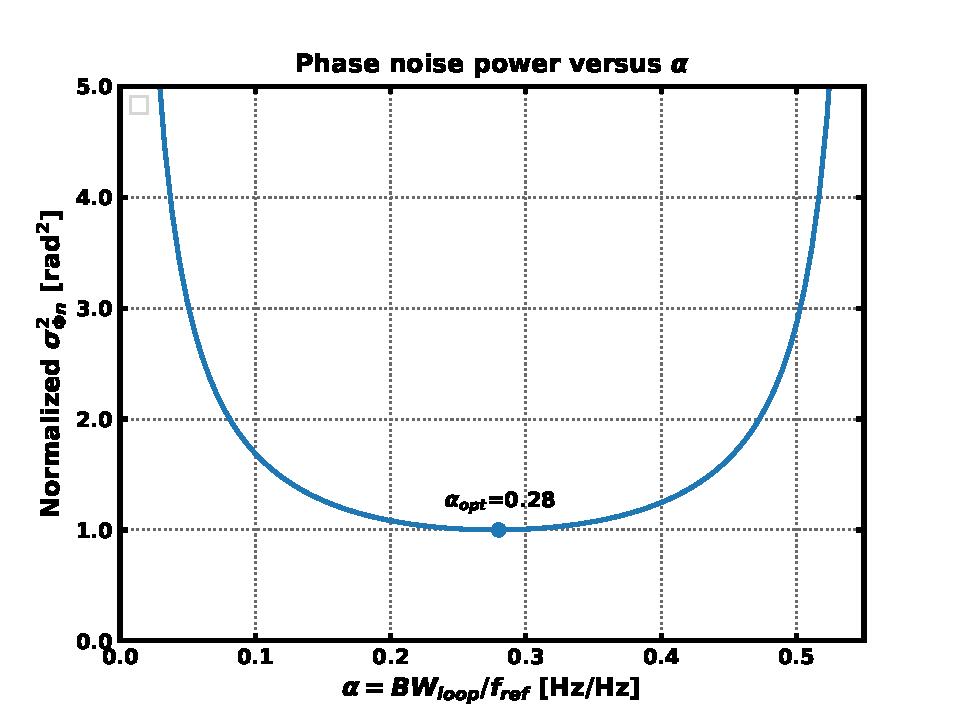
\includegraphics[width=0.6\textwidth, angle=0]{./figs/design/alpha_v_pn}
				\caption{Phase noise power (normalized) versus $\alpha$.}
				\label{fig:alpha_v_pn}
			\end{figure}

			It is possible to derive a constraint for BBPD jitter $\sigma^2_{\phi_j}$ in terms of $\alpha$ and a target $\sigma^2_{\phi_n}$ (i.e. CNR value), providing a performance specification for the design of the physical BBPD. Equation \ref{eq:bbpd_jit_pn} defines the maximum allowable phase noise power due to BBPD jitter, and equation \ref{eq:bbpd_t_jit_rms} defines the maximum RMS jitter in time of the same detector. 
			% In the case of 816 MHz operation, with 12 dB of CNR, and $\alpha$ = 0.1, the maximum allowable RMS BBPD jitter is $\sigma_{t_j}$ = 4.75 ps.
			\begin{equation}\label{eq:bbpd_jit_pn}
				\sigma^2_{\phi_j} \leq \sigma^2_{\phi_n}\left[\frac{4\sqrt{3+\sqrt{10}}}{5\pi^2\alpha} +\frac{2}{\pi} - 1 \right] - \frac{2S_{0_{osc}}(3 + \sqrt{10})}{5\pi\alpha^2f_{ref}}
			\end{equation}
			\begin{equation}\label{eq:bbpd_t_jit_rms}
				\sigma_{t_j} \leq \frac{\sigma_{\phi_n}}{2\pi f_{osc}}\sqrt{\left[\frac{4\sqrt{3+\sqrt{10}}}{5\pi^2\alpha} +\frac{2}{\pi} - 1 \right] - \frac{2S_{0_{osc}}(3 + \sqrt{10})}{5\pi\alpha^2f_{ref}}}
			\end{equation}

			Now with theory in place to optimize PLL performance, mapping of the optimal parameter $K$ onto the loop filter of equation \ref{eq:pi_pll_tf} will be considered. Recall that $\omega_z = K_i/K_p = \sqrt{K}/2\zeta$ and $K = 2\pi K_{BBPD}K_{DCO}K_{i}$. The parameters $K_i$, $K_p$, and $\omega_z$ are thus provided in equations \ref{eq:wz_}-\ref{eq:ki_}.
			\begin{align}
				\omega_z &= \frac{\sqrt{K}}{2}\label{eq:wz_}\\
				K_p &= \frac{\sqrt{K}}{\pi K_{BBPD}K_{DCO}} = \frac{\sqrt{K}\sqrt{\sigma^2_{\phi_j} + \sigma^2_{\phi_n}}}{\sqrt{2\pi}K_{DCO}}\\
				K_i &= \frac{K}{2\pi K_{BBPD}K_{DCO}} = \frac{K\sqrt{\sigma^2_{\phi_j} + \sigma^2_{\phi_n}}}{2\sqrt{2\pi}K_{DCO}}\label{eq:ki_}
			\end{align}
			Converting the filter design into the discrete time equivalent results in equations \ref{eq:b0} and \ref{eq:b1}
			\begin{align}
				b_0 &= \frac{\sqrt{K}\sqrt{\sigma^2_{\phi_j} + \sigma^2_{\phi_n}}}{\sqrt{2\pi}K_{DCO}}\left(1+\frac{\sqrt{K}}{2f_{ref}}\right)\label{eq:b0}\\
				 b_1 &=  - \frac{\sqrt{K}\sqrt{\sigma^2_{\phi_j} + \sigma^2_{\phi_n}}}{\sqrt{2\pi}K_{DCO}}\label{eq:b1}
			\end{align}
			If design of the PLL has a fixed target for $\sigma^2_{\phi_n}$ (CNR), a known $\sigma^2_{\phi_j}$ for the BBPD, and $\alpha$ is selected to be constant (e.g. $\alpha$ = 0.1), the filter coefficients may be calculated as in equations \ref{eq:b0_} and \ref{eq:b1_}.

			\begin{align}
				b_0 &= \frac{\alpha f_{ref}\sqrt{2\pi}\sqrt{\sigma^2_{\phi_j} + \sigma^2_{\phi_n}}}{\sqrt{3+\sqrt{10}}K_{DCO}} \left(1+\frac{\pi\alpha}{\sqrt{3+\sqrt{10}}}\right)\label{eq:b0_}\\
				 b_1 &= - \frac{\alpha f_{ref}\sqrt{2\pi}\sqrt{\sigma^2_{\phi_j} + \sigma^2_{\phi_n}}}{\sqrt{3+\sqrt{10}}K_{DCO}}\label{eq:b1_}
			\end{align}
			% {\color{white}.}

%%%%%%%%%%%%%%%%%%%%%%%%%%%%%%%%%%%%%%%%%%%%%%%%%%%

			\FloatBarrier\subsection{Emergent Bang-Bang PLL Phase Noise}%\label{sec:bb_noise}
			% \FloatBarrier

		\begin{figure}
			\center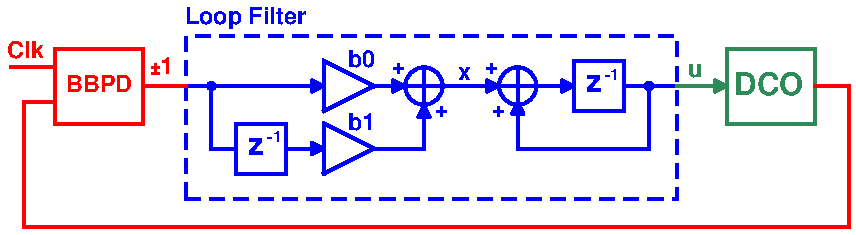
\includegraphics[width=0.8\textwidth, angle=0]{./figs/design/simplified_bbpll}
			\caption{Simplified model of BBPD-PLL}
			\label{fig:simp_bbpdpll}
		\end{figure}
		Since the output of BBPD is quantized to $\pm$ 1, the use of a PI loop filter architecture results in only 4 possible values that node {\color{blue}\textbf{x}} can be valued as shown in the simplified BBPD-PLL model of figure \ref{fig:simp_bbpdpll}. These are $(b_0+b_1)$, $(b_0-b_1)$, $(-b_0+b_1)$, and $(-b_0-b_1)$. The result of this is the loop filter output {\color{teal}\textbf{u}} must increment by one of these four values every reference cycle. 

		The worst case scenario of this is the BBPD outputting an alternating sequence of +1/-1/+1/-1..., for which the output will toggle by increments $(b_0-b_1 )$ and $(-b_0+b_1)$, alternating every cycle. In terms of frequency, the output will either alternate up or down by $K_{DCO}| b_0-b_1 |$ every cycle, which can be substantial depending on the product of those factors. In the phase domain, this results in a cyclostationary triangle wave-like phase trajectory (ignoring other sources of phase noise), as shown in figure \ref{fig:cylostationary}. The worst case increment in phase per cycle is given in equation \ref{eq:cyclo_dph}. In the frequency domain, this cyclostationary behavior can result in spurs, as shown in figure \ref{fig:cylostationary_spurs}. When phase noise from other processes in the PLL are large enough that the they dwarf the worst case cyclostationary behavior, it is expected that the output of the BBPD will be stochastically scrambled and the cyclostationary effects will be subsided. 

		\begin{equation}\label{eq:cyclo_dph}
			\Delta \Phi = \frac{2\pi|b_0-b_1|K_{DCO}}{f_{ref}}
		\end{equation}

	\begin{figure}[htb!]
	    \centering
	    \begin{subfigure}{0.5\textwidth}
	        \centering
	        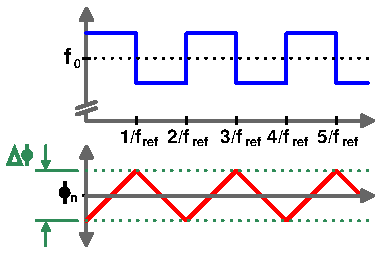
\includegraphics[width=0.8\textwidth, angle=0]{./figs/bbpd_resolution_phase_walk}
	        \caption{ }
	        \label{fig:cylostationary}
	    \end{subfigure}%
	    \begin{subfigure}{0.5\textwidth}
	        \centering
	        \center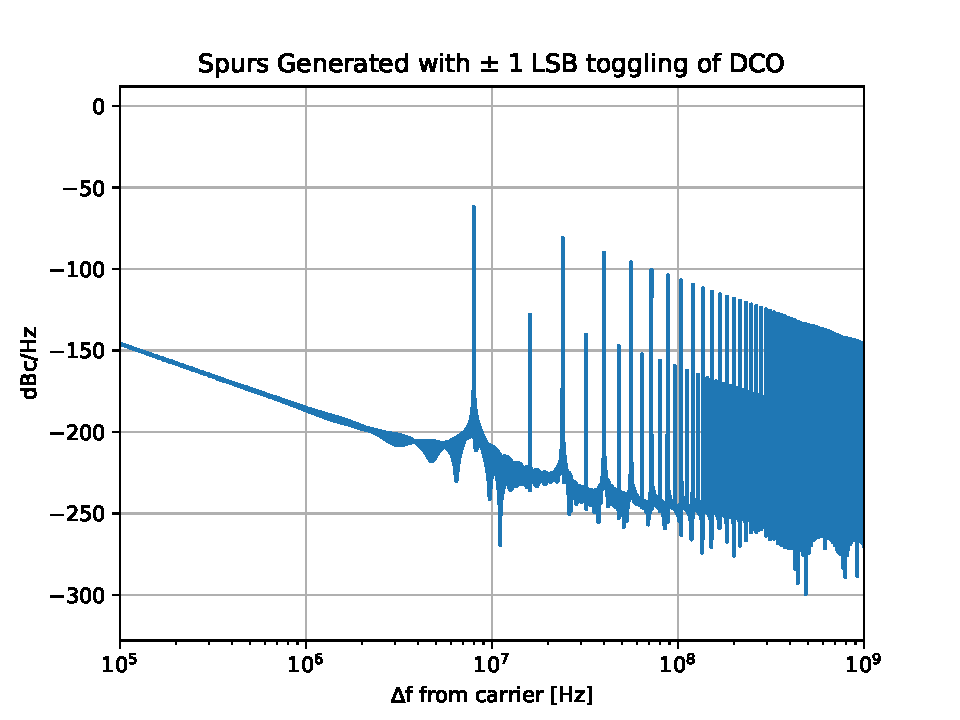
\includegraphics[width=0.8\textwidth, angle=0]{./figs/spurs_dco}
	        \caption{ }
	        \label{fig:cylostationary_spurs}
	    \end{subfigure}
	    \caption{\textbf{(a)} Worst case cyclostationary behavior of BBPD-PLL, \textbf{(b)} Resulting spurs from worst case cyclostationary behavior.}
	    \label{fig:cyclostationary_nonsense}
	\end{figure}


	Even if cyclostationary effects are avoided, the quantization of the loop filter output to increments of the four aforementioned values results in an additive phase noise contribution to the PLL. These increments result in a forced deterministic change in output phase error in every reference interval. The RMS contribution of phase noise to the PLL output due to the quantized steps in frequency from bang-bang operation  has the relationship given in equation \ref{eq:bb_jitter}. This phase noise component will be termed "emergent bang-bang phase noise", represented by $\Phi_{n_{em}}$. Optimization of the PLL with inclusion of emergent bang-bang phase noise contributions will now be considered in the following section. 

		\begin{equation}\label{eq:bb_jitter}
			\sigma_{\Phi_{n_{em}}} \approx \frac{\pi|b_0-b_1|K_{DCO}}{f_{ref}}
		\end{equation}



	\FloatBarrier\subsubsection{Filter Optimization (Emergent Bang-Bang PLL Phase Noise)}\label{sec:bb_noise}
	To optimize the PLL loop filter design for emergent bang-bang effects, the phase noise contribution for this component must be determined. Based on the findings of the previous section, equation \ref{eq:bb_jitter} is modified by adding a proportionality constant $\beta_1$, resulting in equation \ref{eq:bb_jitter_}. The value of this proportionality constant has been computed through simulation, as is later detailed.
		\begin{equation}\label{eq:bb_jitter_}
			\sigma_{\Phi_{n_{em}}} = \beta_1\frac{\pi|b_0-b_1|K_{DCO}}{f_{ref}}
		\end{equation}

	Based on equations \ref{eq:b0_} and \ref{eq:b1_}, the quantity $|b_0-b_1|$ found to be that in equation \ref{eq:b1_b0}. It will be shown that $\alpha$ is a constant under optimal conditions, so the optimized $|b_0-b_1| = 2\beta_2|b_1|$, where $\beta_2$ is a constant proportionality factor. Lumping proportionality constants together, we define $\beta = \beta_1\beta_2$, thus $\sigma_{\Phi_{n_{em}}}$ is defined in equation \ref{eq:bb_jitter2}.
	\begin{equation}\label{eq:b1_b0}
			|b_0-b_1| = \left(2 + \frac{\pi \alpha}{\sqrt{3+\sqrt{10}}}\right)|b_1| = 2\beta_2|b_1|
	\end{equation}
	\begin{equation}\label{eq:bb_jitter2}
		\sigma_{\Phi_{n_{em}}} = \frac{2\pi \beta |b_1|K_{DCO}}{f_{ref}}
	\end{equation}	
	Including $\sigma^2_{\Phi_{n_{em}}}$, BBPD noise and oscillator noise, the total phase noise $\sigma^2_{\Phi_{n}}$ out of the PLL is in equation \ref{eq:bb_osc_noise}.
	\begin{equation}\label{eq:bb_osc_noise}
		\sigma_{\Phi_{n}}^2 = \sigma_{\Phi_{n,DCO}}^2 + \sigma^2_{\Phi_{n_{BBPD}}} + \sigma^2_{\Phi_{n_{em}}} = S_{0_{osc}}\frac{\pi^2}{\sqrt{K}} + \sigma^2_{\phi_n}\frac{5\sqrt{K}}{4f_{ref}}\cdot\left(\frac{\pi}{2}-1\right)  + \sigma^2_{\Phi_{n_{em}}}
	\end{equation}
	Redefining equation \ref{eq:b1} using equation \ref{eq:bb_osc_noise} as the phase noise power results in equation \ref{eq:b1__}.
		\begin{align}\label{eq:b1__}
			 b_1 &=  - \frac{\sqrt{K}\sqrt{\sigma_{\Phi_{n,em}}^2 + \sigma_{\Phi_{n,DCO}}^2 + \sigma^2_{\Phi_{n_{BBPD}}} }}{\sqrt{2\pi}K_{DCO}} \\
			 & = - \frac{\sqrt{K}\sqrt{ \sigma^2_{\Phi_{n_{em}}} +  S_{0_{osc}}\frac{\pi^2}{\sqrt{K}} + \sigma^2_{\phi_n}\frac{5\sqrt{K}}{4f_{ref}}\left(\frac{\pi}{2}-1\right)}  }{\sqrt{2\pi}K_{DCO}}
		\end{align}
	An expression for $\sigma^2_{\Phi_{n_{em}}}$ given in equation \ref{eq:total_pn_pow} is obtained by solving the system of equations formed by equations \ref{eq:bb_jitter2} and \ref{eq:b1__}. Redefining $K$ in terms of $\alpha$ as defined by equation \ref{eq:k_alpha} results in the latter portion of the equation.
	 	\begin{equation}\label{eq:total_pn_pow}
	 		\sigma^2_{\Phi_{n}} = \frac{S_{0_{osc}}\frac{\pi^2}{\sqrt{K}}}{1 + \frac{2\pi K \beta^2}{f_{ref}^2} - \frac{5\sqrt{K}}{4f_{ref}} \left(\frac{\pi}{2}-1\right)}  
	 		= \frac{\frac{\pi S_{0_{osc}}\sqrt{3+\sqrt{10}}}{2f_{ref}}}{\alpha - \alpha^2\frac{5\pi}{2\sqrt{3+\sqrt{10}}}\left(\frac{\pi}{2}-1\right) - \alpha^3 \frac{8\pi^3\beta^2}{3+\sqrt{10}}}
	 	\end{equation}
	To minimize total phase noise power, $d\sigma^2_{\Phi_{n}}/d\alpha = 0$ is solved for, to yield the expression in equation \ref{eq:opt_alpha_beta} for optimal value of $\alpha$.
	\begin{equation} \label{eq:opt_alpha_beta}
		\alpha_{opt} = -\frac{5\sqrt{3+\sqrt{10}}}{48\pi^2\beta^2}
		+ \frac{1}{2}\sqrt{ \frac{25(3+\sqrt{10})}{24^2\pi^4\beta^4}\left(\frac{\pi}{2}-1\right)^2 + \frac{3+\sqrt{10}}{6\pi^3\beta^2}} 
	\end{equation}
	\begin{equation}
		K_{opt} = \frac{(2\pi\alpha_{opt} f_{ref})^2}{3+\sqrt{10}}
	\end{equation}
	Computation of the value of constant $\beta$ is not straightforward, so it has been solved numerically through discrete time simulation of a PLL with a BBPD and PI-controller. This was obtained via a behavioral simulation in steady state over 1000000 reference cycles, with $\beta$ varied until the prediction of $\sigma^2_{\Phi_{n_{em}}}$ and its value from simulation converged within a tolerance of 10$^{-5}$. It has been determined that at the optimum, $\beta_{opt}$ = 0.895 and accordingly $\alpha_{opt}$ = 0.0847. Furthermore, $\beta_1$ = 0.850 and $\beta_2$ = 1.053. These values were observed to be independent of PLL frequency, oscillator phase noise, reference frequency and DCO gain. An example case of this simulation is shown in figure \ref{fig:em_bb_pn}, where the ratio $\beta_1$ of equation \ref{eq:bb_jitter_} is seen with the vertical lines. Figure \ref{fig:opt_alpha_full} shows the effect of $\alpha$ versus total integrated phase noise power. Total phase noise power grows asymptotically with $\alpha$ = 0 and $\alpha$ = 0.1503. 

	\begin{figure}[htb!]
	    \centering
	    \begin{subfigure}{0.5\textwidth}
	        \centering
	        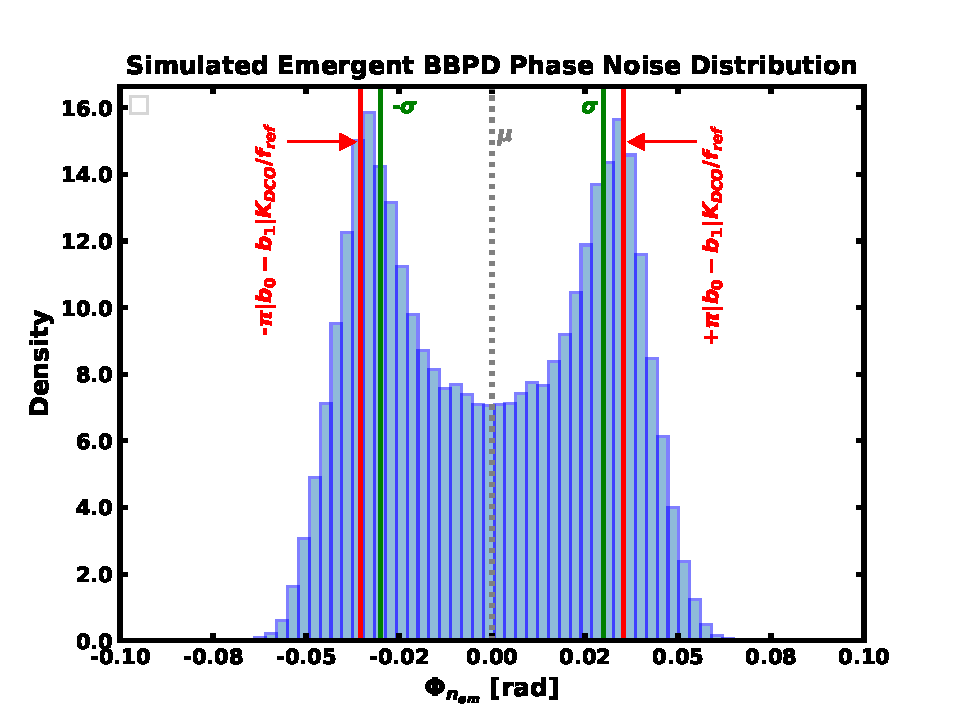
\includegraphics[width=1\textwidth, angle=0]{./figs/design/em_bb_pn}
	        \caption{ }
	        \label{fig:em_bb_pn}
	    \end{subfigure}%
	    \begin{subfigure}{0.5\textwidth}
	        \centering
	        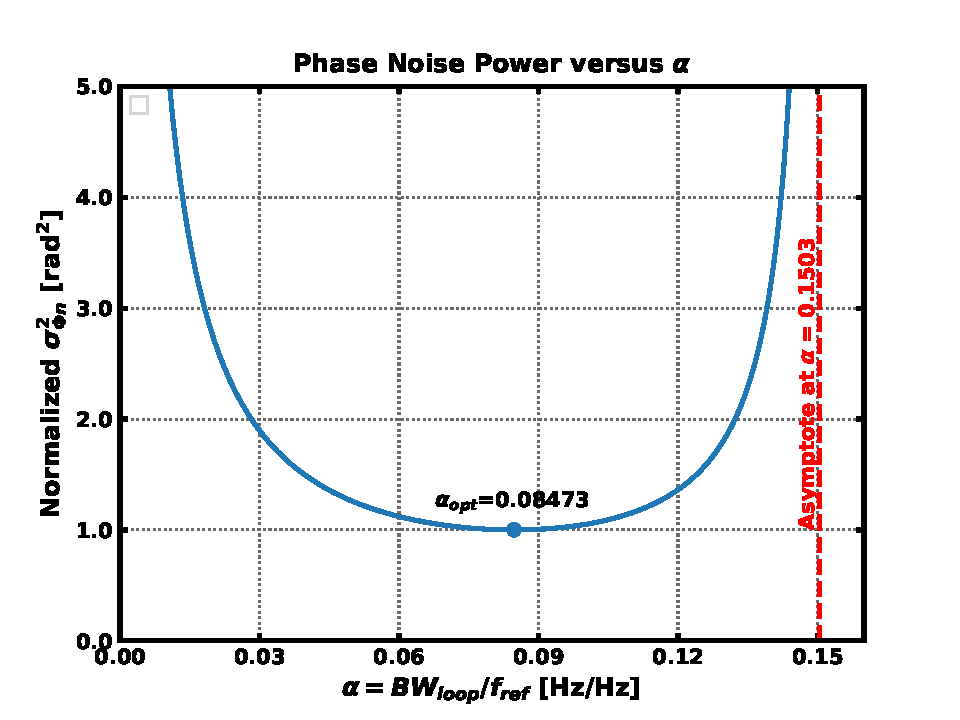
\includegraphics[width=1\textwidth, angle=0]{./figs/design/opt_alpha_full}
	        \caption{ }
	        \label{fig:opt_alpha_full}
	    \end{subfigure}
	    % \caption{x.}
	    \label{fig:alph_opt}
	    \caption{\textbf{(a)} Simulated emergent bang bang phase noise component of PLL phase noise, \textbf{(b)} Total output phase noise (normalized) versus $\alpha$.}
	\end{figure} 

Application of the determined optimal parameters into equation \ref{eq:total_pn_pow} results in equation \ref{eq:optimal_pn_pow}. 

	\begin{equation}\label{eq:optimal_pn_pow}
		\left.\sigma_{\Phi_{n}}^2\right|_{\alpha_{opt}} = 74.79376\cdot\frac{S_{0_{osc}}}{f_{ref}} = 74.79376\cdot \frac{\mathcal{L}_{osc}(f)f^2}{f_{ref}} \hspace{0.5em} [\textnormal{rad}^2]
	\end{equation}





	% In the case of this work with a target of 2.448 GHz, 16 MHz reference, 100 $\mu$W power, and 300K ambient temperature, the theoretical obtainable CNR is 21.4 dB, or $\sigma_{\Phi_{n}}^2$ = 0.012 rad$^2$.
	Computed discrete time filter coefficients for this optimization case are provided in equations \ref{eq:b0_bb} and \ref{eq:b1_bb}.
	\begin{align}
		b_0 &= \frac{\alpha_{opt}\sqrt{74.79376\cdot2\pi S_{0_{osc}} f_{ref}}}{K_{DCO}\sqrt{3+\sqrt{10}}}\left(1+\frac{\pi\alpha_{opt}}{\sqrt{3+\sqrt{10}}}\right)\label{eq:b0_bb}\\
		&= 0.8186975 \frac{\sqrt{S_{0_{osc}} f_{ref}}}{K_{DCO}}\\
		b_1 &= -\frac{\alpha_{opt}\sqrt{74.79376\cdot2\pi S_{0_{osc}} f_{ref}}}{K_{DCO}\sqrt{3+\sqrt{10}}} \label{eq:b1_bb}\\
		&=-0.739456 \frac{\sqrt{S_{0_{osc}} f_{ref}}}{K_{DCO}}
	\end{align}

	\subsubsection{Choice of Optimization Strategy}
	Depending on the implementation, the noise contributions from the phase detector jitter may exceed the emergent bang bang phase noise components. This may be the case in high frequency PLLs, e.g. mm-wave PLLs, where cycle periods are short. For 2.4 GHz operation in 22nm technology, this poses less of a problem. In this work, two optimization theories have been provided, for different noise regimes. The optimization theory of section \ref{sec:bb_noise} ignores detector jitter while considering emergent effects, and section \ref{sec:opt_lf_noisy_bbpd} ignores emergent bang-bang behavior, while considering BBPD jitter. The recommended strategy for filter design is therefore to calculate the optimal filter design using both theories, and select the one that results in a larger total phase noise value $\sigma_{\Phi_{n}}^2$, as that will be the dominant noise mode. 

	In this work, using a -158.9 dB oscillator phase noise FOM at 2.448 GHz with 90$\mu$W of power, a 16 MHz reference, $K_{DCO}$ = 4.2 kHz/LSB, and a detector jitter of 1.342 ps RMS, leads to a CNR of 15.5 dB when optimizing for oscillator plus jitter-inclusive BBPD noise, and a CNR of 13.6 dB when optimizing for oscillator noise plus emergent bang bang phase noise and jitterless detector noise. Selecting the worse valued result as the accurate model for this implementation then implies that this work should be optimized with the emergent bang-bang phase noise model.

	The final optimized filter parameters for the design of this work are in the results section \ref{sec:rec_lf}.


% ################################################################################################
% ################################################################################################



	% \FloatBarrier

	% 	\subsubsection{Filter Design for Synchronous counter}
	% 		As gear-switching is intended to be used in this work, a separate loop filter will be calculated that is optimized for settling time (i.e. lock time) with the synchronous counter phase detector during initial start up. It was determined in the previous section that the poles of the PI-PLL occur at s = $\zeta\sqrt{K} \pm j\sqrt{K}\sqrt{1-\zeta^2}$, as a conjugate pair. Taking the real portion (same for both) provides for the value of the PLL time constant:
	% 		\begin{equation}
	% 			\tau = \frac{1}{|\min(\Re(\{s_{p1}, s_{p2}\}))|} = \frac{1}{\zeta\sqrt{K}}
	% 		\end{equation}
	% 		If $\delta$ is considered the fraction of the initial frequency error during the lock process that may be described as being in-lock, then the PLL lock time is given by equation \ref{eq:locktime}. $\delta$ can be also stated in terms of initial frequency error $\Delta f$, and the frequency tolerance from steady state $f_{tol}$ that is considered to be in lock for a given application.
			% \begin{equation}\label{eq:locktime}
			% 	t_s = \frac{-\ln(\delta)}{\zeta\sqrt{K}} = \frac{-\ln\left(\frac{f_{tol}}{|\Delta f|}\right)}{\zeta\sqrt{K}}
			% \end{equation}
	% 		It is observed that lock time is decreased by increasing the value of both $\zeta$ and $K$. Again, the constraint $\zeta$=1 is used due to its favorable characteristics. Thus, it is of interest here to maximize the value of $K$. It is seen that in equation \ref{eq:loop_bw} that $K\propto BW_{loop}^2$, thus loop bandwidth should be maximized. Again defining a constraint between loop bandwidth and reference frequency of $\alpha = BW_{loop}/f_{ref}$, equation \ref{eq:k_alpha} can be used to determine the optimal selection of $K$ for a given $\alpha$ and $f_{ref}$. Plugging this into equation \ref{eq:locktime} yields equation \ref{eq:locktime2}.
	% 		\begin{equation}\label{eq:locktime2}
	% 			t_s =  \frac{-\sqrt{3+\sqrt{10}}\ln\left(\frac{f_{tol}}{|\Delta f|}\right)}{2\pi\alpha f_{ref}}
	% 		\end{equation}
	% 		Now, these defined filters parameters will be translated into a filter design. Again, the definitions $K=2\pi K_{PD}K_{DCO}K_{i}$ and $\omega_z = K_i/K_p$ are used. A detector gain $K_{PD}$ must be defined first for the synchronous counter. Since the synchronous counter counts cycles, it in effect converts $2\pi$ of phase into an increment of count of 1. Thus the gain is:
	% 		\begin{equation}
	% 			K_{PD} = \frac{1}{2\pi}
	% 		\end{equation}
	% 		The parameters $K_i$, $K_p$ and $\omega_z$ are then solved for, to result in equations \ref{eq:kp_sc} to \ref{eq:b1_sc}.
	% 		\begin{align}
	% 			K_p & = \frac{4\pi\alpha f_{ref}}{\sqrt{3+\sqrt{10}}K_{DCO}}\label{eq:kp_sc}\\
	% 			K_i & = \frac{(2\pi\alpha f_{ref})^2}{(3+\sqrt{10})K_{DCO}}\\
	% 			\omega_z &= \frac{\pi\alpha f_{ref}}{\sqrt{3+\sqrt{10}}}\label{eq:wz_sc}\\
	% 			b0 &= K_p = \frac{4\pi\alpha f_{ref}}{\sqrt{3+\sqrt{10}}K_{DCO}}  \\
	% 			b1 &= \frac{4\pi\alpha f_{ref}}{\sqrt{3+\sqrt{10}}K_{DCO}}\left( 1 + \frac{\pi\alpha}{\sqrt{3+\sqrt{10}}} \right ) \label{eq:b1_sc}\\
	% 		\end{align}

		% \subsubsection{PI-controller Phase Margin}\label{pi_phase_margin}
		% 	The PI-PLL architecture of this work has a phase margin determined by the damping ratio $\zeta$, given by equation \ref{eq:pm_pi_pll}. Figure \ref{fig:phase_margin} shows phase margin versus $0 \geq \zeta \geq 1$ of the PI-controller PLL. It is recommended to use at least 30-60 degrees in phase margin to achieve stability \cite{ogata_2010_stability}. In this work, $\zeta$ = 1 has been used, so a phase margin of 76 degrees is expected, and accordingly stability should be expected.
		% 	\begin{equation}\label{eq:pm_pi_pll}
		% 		\angle \text{L}(\omega_{ug}) = \frac{180}{2\pi}\arctan\left(2\zeta\sqrt{2\zeta^2 + \sqrt{4\zeta^4+1}}\right)\hspace{1em}[\text{degrees}]
		% 	\end{equation}
		% 	\begin{figure}[htb!]
		% 		\center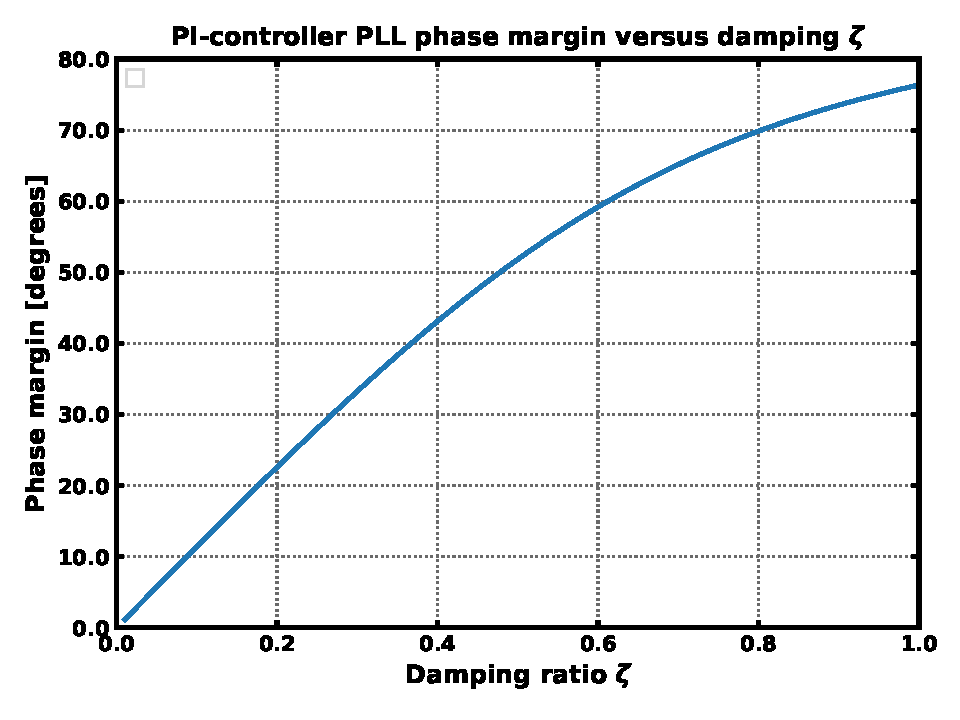
\includegraphics[width=0.5\textwidth, angle=0]{figs/damping_vs_pm.pdf}
		% 		\caption{PI-controller PLL phase margin versus damping ratio.}
		% 		\label{fig:phase_margin}
		% 	\end{figure}



	% \subsubsection{Discretization of Loop Filter}\label{disc_lf_comp_pi}
	% 	Using the continuous filter discretization approach described in section \ref{lf-discretization} on the loop filter of equation \ref{eq:pi_pll_tf} results in equation \ref{eq:z_lf}.
	% 	\begin{align}
	% 		\textnormal{H}_{LF}(z) & = \left.\frac{K_i}{s}\left(\frac{s}{\omega_z} + 1\right)\right\vert_{s=\frac{1}{\Delta T_s}(1-z^{-1})}
	% 		&= K_p\frac{(1+\omega_z\Delta T_s)-z^{-1}}{1- z^{-2}}\label{eq:z_lf}
	% 	\end{align}

	% 	The transformation of equation \ref{eq:z_lf} into a digitally implementable design as a direct form 1 IIR filter shown in figure \ref{fig:filt_imple}. Its filter coefficients given by equations \ref{eq:b0} and \ref{eq:b1}.
	% 	\begin{figure}[htb!]
	% 		\center\fontfamily{\sfdefault}\selectfont
% XCircuit output "filter_arch_pi.tex" for LaTeX input from filter_arch_pi.ps
\def\putbox#1#2#3#4{\makebox[0.00000in][l]{\makebox[#1][l]{}\raisebox{\baselineskip}[0.00000in][0.00000in]{\raisebox{#2}[0.00000in][0.00000in]{\scalebox{#3}{#4}}}}}
\def\rightbox#1{\makebox[0.00000in][r]{#1}}
\def\centbox#1{\makebox[0.00000in]{#1}}
\def\topbox#1{\raisebox{-0.60\baselineskip}[0.00000in][0.00000in]{#1}}
\def\midbox#1{\raisebox{-0.20\baselineskip}[0.00000in][0.00000in]{#1}}
   \scalebox{1}{
   \normalsize
   \parbox{5.54167in}{
   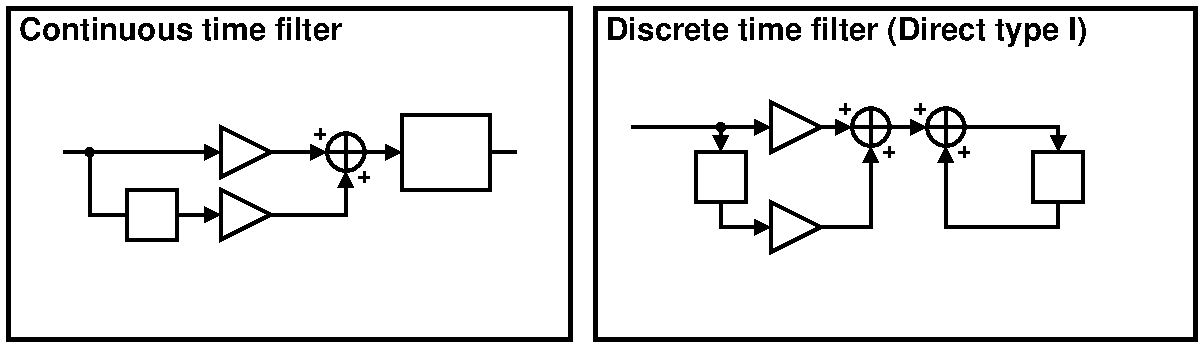
\includegraphics[scale=0.70000]{./figs/filter_arch_pi.pdf}\\
   % translate x=1728 y=944 scale 0.38
   \putbox{1.91800in}{0.90300in}{0.96}{$\frac{1}{\frac{s}{\omega_p} + 1}$}%
   \putbox{1.14800in}{1.01500in}{0.96}{$K_p$}%
   \putbox{1.14800in}{0.72800in}{0.96}{$K_i$}%
   \putbox{0.60900in}{0.58100in}{0.96}{$1/s$}%
   \putbox{0.25900in}{0.98700in}{0.96}{x[n]}%
   \putbox{2.35900in}{0.98700in}{0.96}{y[n]}%
   \putbox{2.92600in}{1.10600in}{0.96}{x[n]}%
   \putbox{4.99800in}{1.01500in}{0.96}{\rotatebox{-360}{y[n]}}%
   \putbox{3.26200in}{0.75600in}{0.96}{$z^{-1}$}%
   \putbox{3.73100in}{1.13400in}{0.96}{b$_0$}%
   \putbox{3.73100in}{0.66500in}{0.96}{b$_1$}%
   \putbox{4.83700in}{0.75600in}{0.96}{$z^{-1}$}%
   \putbox{4.99800in}{0.55300in}{0.96}{y[n-1]}%
   } % close 'parbox'
   } % close 'scalebox'
   \vspace{-\baselineskip} % this is not necessary, but looks better
\fontfamily{\rmdefault}\selectfont

	% 		\caption{Implementation of filter.}
	% 		\label{fig:filt_imple}
	% 	\end{figure}

	% 	\begin{align}
	% 		b_0 &= K_p (1+\omega_z\Delta T_s)\\
	% 		 b_1 &= -K_p 
	% 	\end{align}
	% 	In the case of a BBPD PLL:
	% 	\begin{align}
	% 		b_0 &= \frac{\sqrt{K}\sqrt{\sigma^2_{\phi_j} + \sigma^2_{\phi_n}}}{\sqrt{2\pi}K_{DCO}}\left(1+\frac{\sqrt{K}}{2f_{ref}}\right)\label{eq:b0}\\
	% 		 b_1 &=  - \frac{\sqrt{K}\sqrt{\sigma^2_{\phi_j} + \sigma^2_{\phi_n}}}{\sqrt{2\pi}K_{DCO}}\label{eq:b1}
	% 	\end{align}
	% 	If design of the PLL is with fixed target for $\sigma^2_{\phi_n}$ (CNR), has a known $\sigma^2_{\phi_j}$ for the BBPD, and $\alpha$ is selected to be constant (i.e. 0.1), the filter coefficients may be calculated as in equations \ref{eq:b0_} and \ref{eq:b1_}.

	% 	\begin{align}
	% 		b_0 &= \frac{\alpha f_{ref}\sqrt{2\pi}\sqrt{\sigma^2_{\phi_j} + \sigma^2_{\phi_n}}}{\sqrt{3+\sqrt{10}}K_{DCO}} \left(1+\frac{\pi\alpha}{\sqrt{3+\sqrt{10}}}\right)\label{eq:b0_}\\
	% 		 b_1 &= - \frac{\alpha f_{ref}\sqrt{2\pi}\sqrt{\sigma^2_{\phi_j} + \sigma^2_{\phi_n}}}{\sqrt{3+\sqrt{10}}K_{DCO}}\label{eq:b1_}
	% 	\end{align}
	% 	%%%%



%%%%%%%%%%%%%%%%%%%%%%%%%%%%%%%%%%%%%%%%


		\subsection{Loop Filter Implementation}

			The loop filter has been implemented digitally as shown in figure \ref{fig:pi_dig_imp}. Due to the fixed output possibilities of the BBPD (digital 0 or 1 corresponding to $\pm$1), the multipliers in the PI-controller have been replaced by multiplexers which select the appropriate signed version of the coefficients \{$b_0$, $b_1$\}, depending on the input sequence to the filter. Replacing the multipliers with multiplexers allows for substantial savings in terms of area and power, due to the significantly lower logical complexity to implement a parallel mux versus an array multiplier. 

			% This approach is intended to reduce dynamic power in steady state operation (using the BBPD). The rationale is that the synchronous counter is a linear detector, thus requires multipliers in the datapath to implement the filter, whereas the BBPD only outputs two values (+1 and -1), so the multipliers can be replaced with multiplexers that select between two sets of possible products ($\pm b_0$ and $\pm b_1$) depending on the input. It is lower energy to operate a multiplexer than an array multiplier due to substantially lower complexity of logic, so in steady state BBPD operation, substantial power savings will be seen. The usage of a common integrator at the output for both detector modes allows for seamless continuity of output value during transition between detector modes. \hl{bbpd mux inputs need to be reversed}
			\begin{figure}[htb!]
			        \centering
			        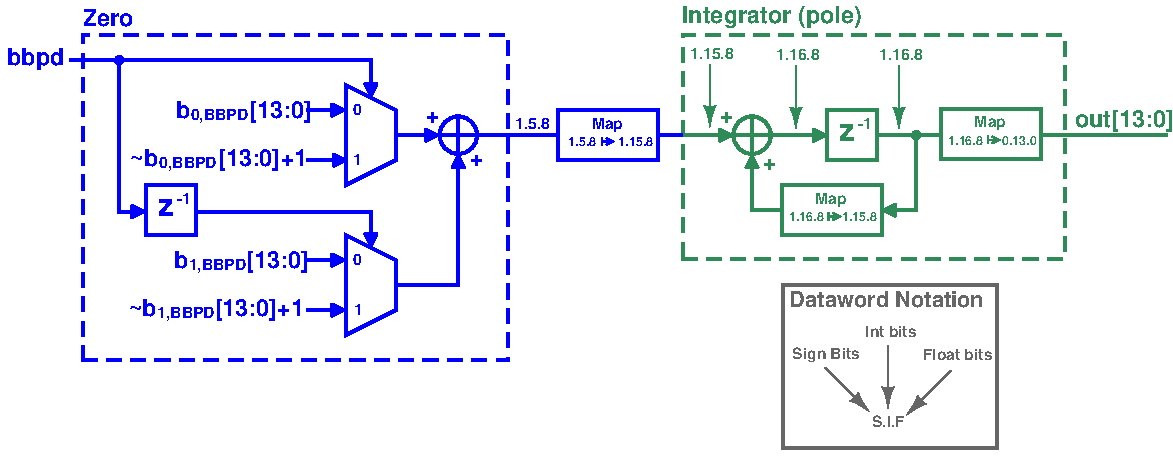
\includegraphics[width=\textwidth, angle=0]{./figs/design/mux_datapath2}
			    \caption{PI-controller implementation for combination of BBPD and synchronous counter usage.}
			    \label{fig:pi_dig_imp}
			\end{figure}

			The computed filter coefficients $\{b_0$, $b_1\}$ for the loop filter are digitized into finite length signed two's complement words. A two's complement data word contains one sign bit, and variable number of bits representing the integer and fractional portions of the encoded number. The author of this work has previously devised a method \cite{Me} for automatically computing the number of bits required to represent a loop filter in an all digital PLL. First, the selection of number of integer bits \texttt{int\_bits} is determined by considering the integer part of the filter coefficients. If the integer portions of the filter coefficients $\{b_0$, $b_1\}$ are divided into positive and negative valued sets \texttt{pos\_ints} and \texttt{neg\_ints}, the total integer bits required is therefore given in equation \ref{eq:int_bits}. Computation of the fractional portion is more complicated, and is based on reducing the quantization noise floor of the loop filter below the phase detector noise level of the PLL. The PLL design framework from \cite{Me} has been used in this work for determining the minimum digitized representation size of filter coefficients. This has been automatically computed such that the filter at most adds 0.1 dB of noise compared to BBPD noise components. Furthermore, the number of bits is optimized to minimize mean squared filter error below a limit, 0.1 dB is used in this work. Results from this optimization are shown in figure \ref{fig:lf_bits_opt}, where it has been found the minimum number of coefficient bits is 10, with 5 integer bits and 4 fractional bits. In order to further reduce quantization noise of the loop filter, the number of fractional bits has been set to 8 bits, bringing the total filter coefficient size to 14 bits. The output integrator of the loop filter has been implemented with 8 fractional bits, and 15 integer bits, where the output to the DCO is tapped of the integer portion of the integrator.

			% It should also be noted that the output integrator is signed, however, the loop filter cannot use a negative control word. Therefore, the sign bit is not used by the DCO, and is rather used as an overflow indicator, implying that the PLL is out of calibration because the loop filter it out of its nominal range. Recalibration can then be triggered by the sign bit.
			\begin{align}
				\mathtt{pos\_int\_bits} &= \left\lfloor \log_2\left(\max\left(\left\lfloor \mathtt{pos\_ints} \right\rfloor\right)\right) \right\rfloor +1\\
				\mathtt{neg\_int\_bits} &= \left\lceil \log_2\left(\max\left(\left\lfloor \mathtt{neg\_ints} \right\rfloor\right)\right) \right\rceil\\
				\mathtt{int\_bits} &= \max(\mathtt{\{pos\_int\_bits}, \mathtt{neg\_int\_bits}\})\label{eq:int_bits}
			\end{align}


	\begin{figure}[htb!]
	    \centering
	    \begin{subfigure}{0.5\textwidth}
	        \centering
	        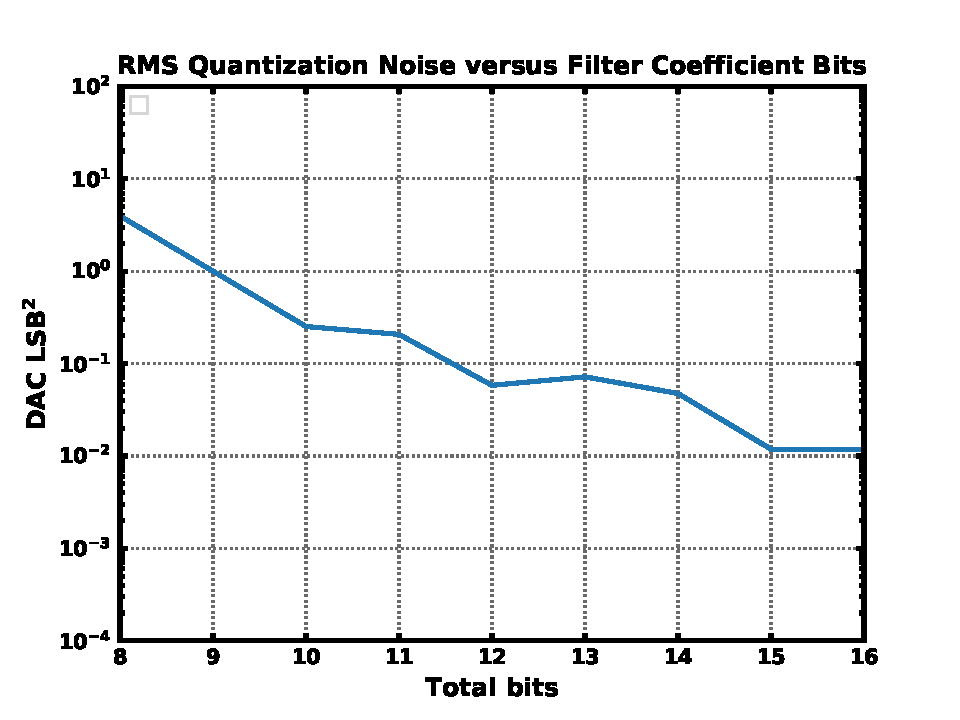
\includegraphics[width=1\textwidth, angle=0]{./figs/design/lf_quant_noise}
	        \caption{ }
	        \label{fig:lf_quant_noise}
	    \end{subfigure}%
	    \begin{subfigure}{0.5\textwidth}
	        \centering
	        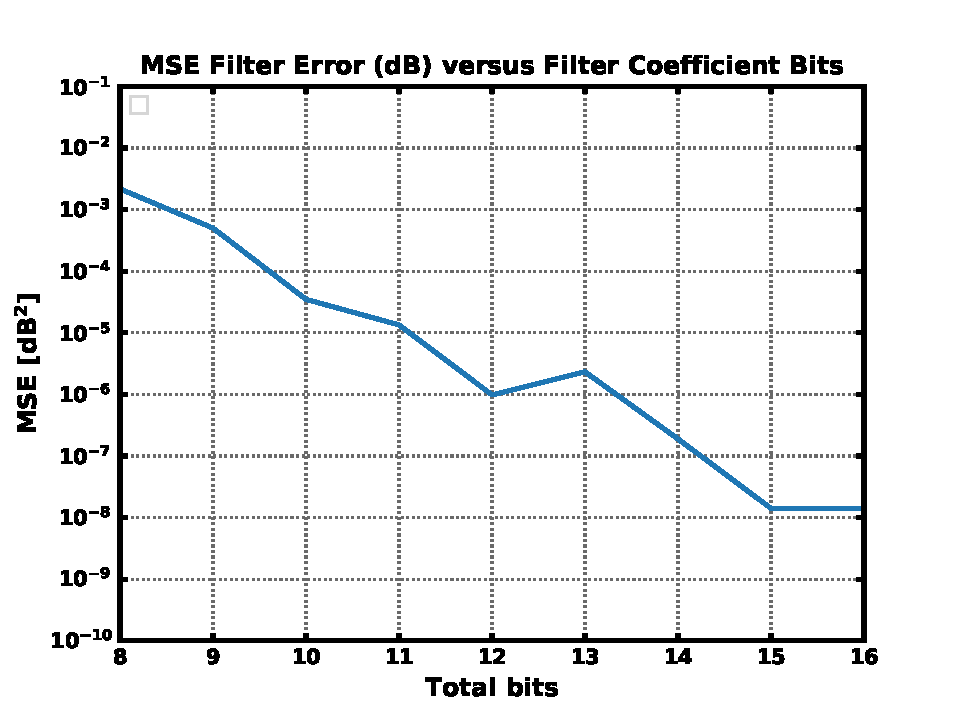
\includegraphics[width=1\textwidth, angle=0]{./figs/design/lf_mse}
	        \caption{ }
	        \label{fig:lf_mse}
	    \end{subfigure}
	    % \caption{x.}
	    \caption{\textbf{(a)} Loop filter quantization noise versus coefficient dataword size, \textbf{(b)} Loop filter MSE versus coefficient dataword size.}
	    \label{fig:lf_bits_opt}
	\end{figure} 

	 The implemented loop filter Verilog hardware description used for logic synthesis is in appendix \ref{sec:lf_verilog}.



			% \begin{figure}[htb!]
			%         \centering
			%         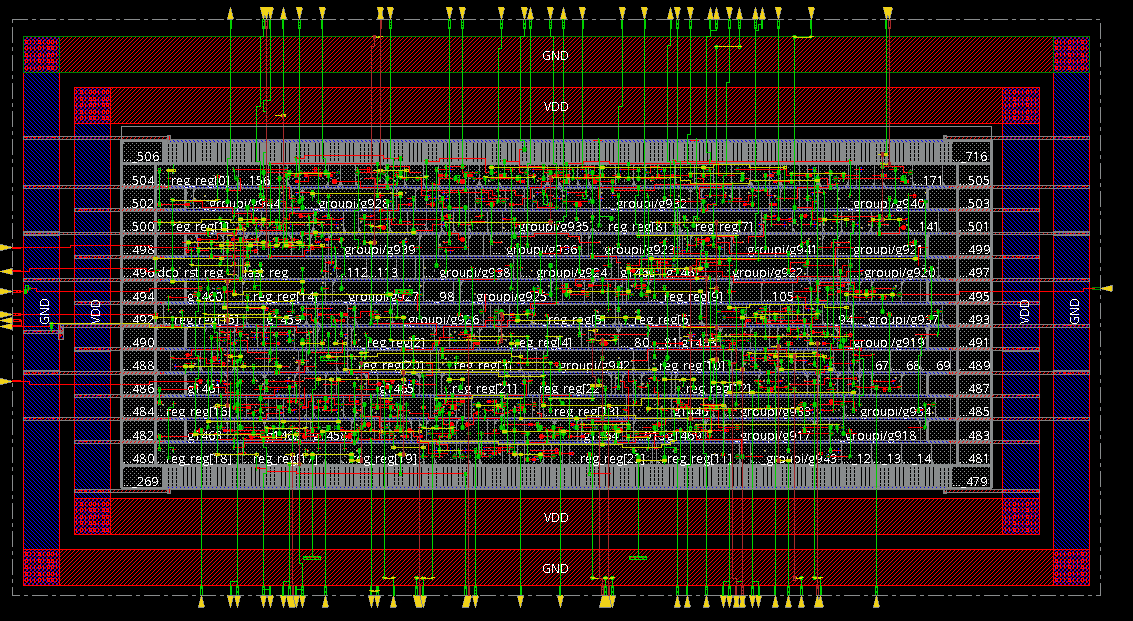
\includegraphics[width=0.9\textwidth, angle=0]{./figs/design/bbpd_lf_only.png}
			%     \caption{Synthesized loop filter.}
			%     \label{fig:bbpd_only_lf_lay}
			% \end{figure}

%%%%%%%%%%%%%%%%%%%%%%%%%%%%%%%%%%%%%%%%%%%%%
% \pagebreak
% \section{phase noise components....}

% 	\begin{figure}[htb!]
% 	    \centering
% 	    \begin{subfigure}{0.5\textwidth}
% 	        \centering
% 	        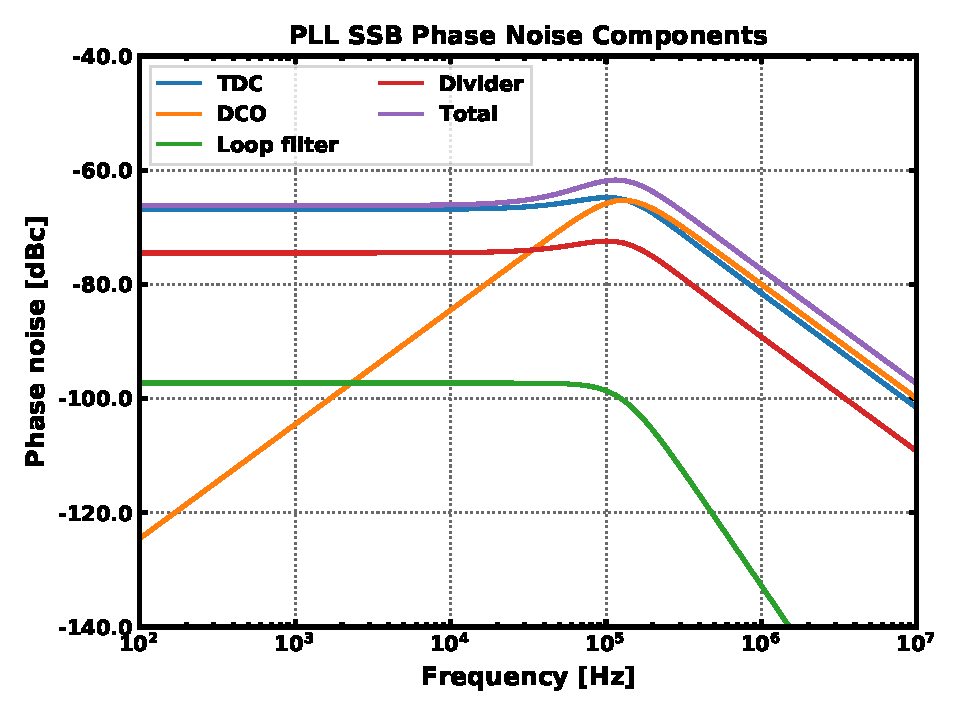
\includegraphics[width=1\textwidth, angle=0]{figs/pn_comps.pdf}
% 	        \caption{ }
% 	        \label{fig:ex_pll_pn_comps}
% 	    \end{subfigure}%
% 	    \begin{subfigure}{0.5\textwidth}
% 	        \centering
% 	        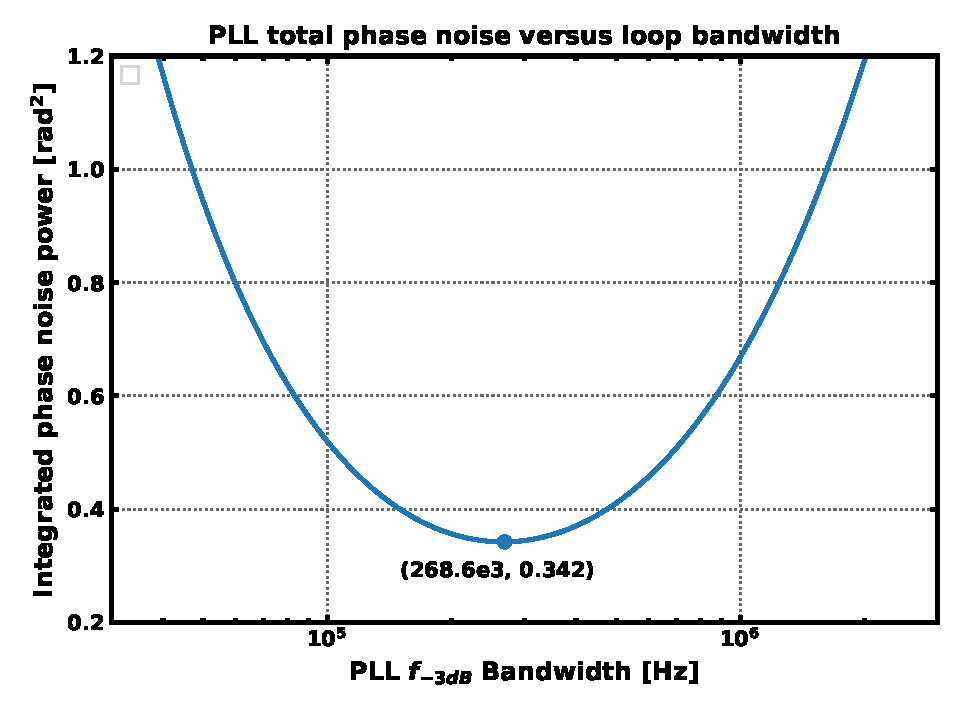
\includegraphics[width=1\textwidth, angle=0]{figs/bandwidth_vs_pn.pdf}
% 	        \caption{ }
% 	        \label{fig:bw_pn_tradeoff}
% 	    \end{subfigure}
% 	    % \caption{Approximate model for ring oscillator inverter delay cell.}
% 	    \label{fig:pll_pn_examples}
% 	    \caption{\textbf{(a)} Example PLL phase noise from models in this work, \textbf{(b)} integrated phase noise power versus bandwidth for the same PLL.}
% 	\end{figure}

% \begin{figure}[htb!]
% 	\center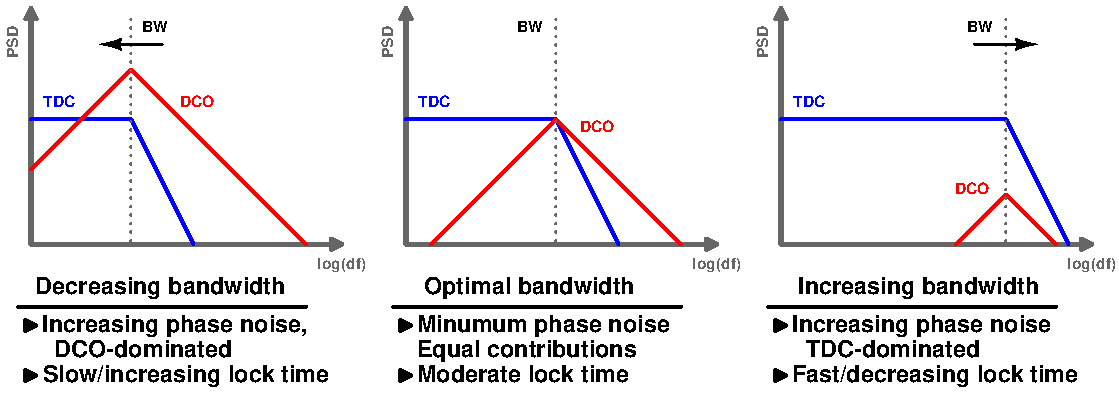
\includegraphics[width=1\textwidth, angle=0]{figs/loop_bandwidth}
% 	\caption{Bandwidth versus total integrated phase noise of PLL.}
% 	\label{fig:bw_vs_pn2}
% \end{figure}




	% \vspace{-3em}
	% \begin{figure}[htb!]
	%     \centering
	%     \begin{subfigure}{0.5\textwidth}
	%         \centering
	%         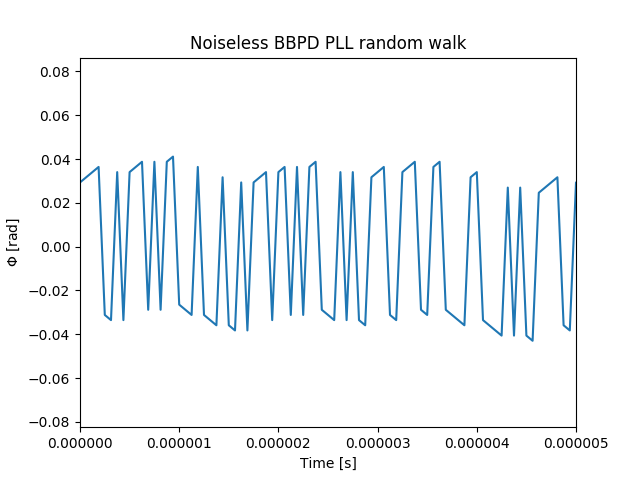
\includegraphics[width=0.8\textwidth, angle=0]{./figs/bbpd_rw}
	%     \end{subfigure}%
	%     \begin{subfigure}{0.5\textwidth}
	%         \centering
	%         \center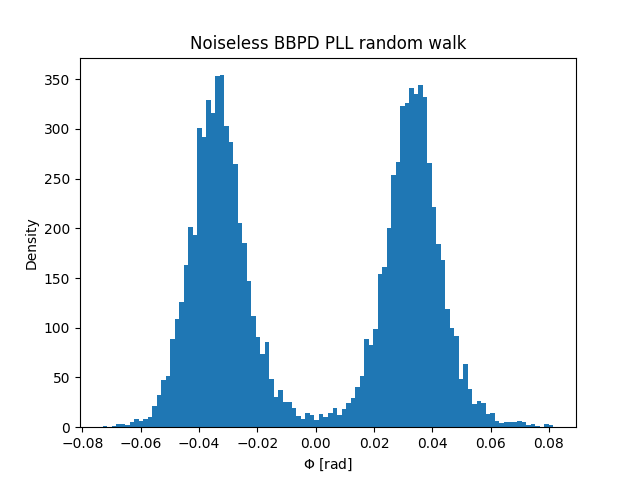
\includegraphics[width=0.8\textwidth, angle=0]{./figs/bbpd_rw_hist}
	%     \end{subfigure}
	%     % \caption{Approximate model for ring oscillator inverter delay cell.}
	% \end{figure}



			% % \vspace{100em}
			% \begin{itemize}[itemsep=4pt,label=\protect---]
			% 	\item Found an interesting dissertation on BBPD PLLs [3], which shows that the linearized BBPD gain model I have been using (K$_{BBPD}$ = $2/\sqrt{2\pi}\sigma_{\Phi_n}$) is not totally correct. 
			% 	\begin{itemize}[itemsep=4pt,label=\protect$\bullet$]
			% 			\item Due to BBPF-PLL resolution jitter, varies depending if resolution jitter or if random noise is the dominant component.
			% 	\end{itemize}
			% 	\item Need to account for this in my filter optimization code...
			% 	\item An approximation, with random/uncorrelated noise with $\sigma_{\Phi uc}$, and resolution jitter $\sigma_{\Phi{rj}}$ (based on variable substitution of [3]'s theory):
			% 	\begin{equation}
			% 		K_{BBPD} = \frac{1}{\sqrt{2\pi}\sigma_{\Phi uc}}\left[1+ e^{-\frac{1}{2}\left(\frac{\sigma_{\Phi{rj}}}{\sigma_{\Phi uc}}\right)^2} \right]
			% 	\end{equation}
			% 		\begin{equation}
			% 			\sigma_{\Phi rj} \approx \frac{\pi|b_0-b_1|K_{DCO}}{f_{ref}}
			% 		\end{equation}
			% 	\item Currently, I should be well into the random noise dominated regime.
			% \end{itemize}






% ################################################################################################
% ################################################################################################

\FloatBarrier {\color{white}.}
\FloatBarrier\pagebreak
\section{DCO Design}\label{sec:dco_design}
The digitally controlled oscillator of this work has been implemented via the digitization of a voltage controlled oscillator (VCO) using digital to analog converters (DACs).  The following sections will describe the implementation of a VCO, and the capacitive DACs used to digitize the VCO. 
% The choice of such a topology was chosen as it was found to permit minimal energy to be expended in the digitization of the oscillator control.

% \FloatBarrier\pagebreak
\subsection{Selection of Oscillator Type}
	Oscillator circuits implemented in CMOS process technologies either fall under the category of resonant LC circuits, or RC based ring and relaxation oscillators. LC circuits provide favorable phase noise performance, as seen in figure \ref{fig:lc_ro_fom}, which shows typical phase noise improvements on the order of 20 dB for published LC designs over RC designs. This is due to the inherent nature of an LC circuit, as the higher the quality factor it has, the narrower the resonance line width and consequent phase noise is. In the ultra-low power domain of this work, however, ring oscillators pose several advantages over LC designs. These include substantially smaller integration area due to no need for integrated inductors, simpler design, convenient rail-to-rail signal levels, and lower achievable minimum power at a given frequency. Also significant is the ability to instantly startup a ring oscillator, which can be achieved with known initial phase if using appropriate phase reset circuitry. In a PLL using a BBPD, the ability to start the oscillator with a known zeroed-phase is highly beneficial. Due the simple nature of the BBPD, it is not possible to detect phase and frequency errors simultaneously, thus if a BBPD-PLL is started with both phase and frequency error, the PLL may not achieve lock. Initial zeroing of phase with a ring oscillator allows for phase uncertainty to be removed at start up, which allows for deterministic locking performance of the BBPD-PLL. With the intent of this design to allow for fast duty cycled operation, the need for deterministic locking and instant start up is imperative, thus, for this reason a ring oscillator topology has been selected for this work. 

	In this work, the ability of the FD-SOI backgate terminal to alter device threshold voltages has been utilized in order to implement a backgate voltage controlled ring oscillator as the main PLL VCO. The design process behind such an oscillator will be described in the following sections. A novel delay cell topology which exploits FD-SOI backgates to implement both differential operation and frequency is subsequently introduced. The described design enables usage of capacitive DACs to set oscillator control voltages, leading to minimal extra power consumption needed to convert the voltage controlled ring oscillator into a DCO.


\FloatBarrier

%%%%%%%%%%%%%%%%%%%%%%%%%%%%%%%%%%%%%%%%%%%%%%%%%%%%%%%%%%%%%%%%%%%%%%%%%%%

\subsection{Ring Oscillator Channel Length Consideration}\label{sec:chan_len_22fdx}
	Scaling of device channel lengths has a great impact on phase noise for ring oscillators. According to \cite{Liu2020}, ring oscillator phase noise takes the form of equation \ref{eq:liu_pn_scaling}. $V_{DD}$ is the supply voltage, $V_t$ is the threshold voltage, $P_{DC}$ is the oscillator power consumption, $\gamma p$ and $\gamma n$ are the respective PMOS and NMOS noise factors, $f_0$ is the oscillator frequency, and $f$ is the offset from the carrier for the phase noise. It is expected that the excess noise factor of the transistor will increase with decreasing channel length \cite{Antonopoulos2013}, thus unavoidably phase noise will also increase with decreasing length following equation \ref{eq:liu_pn_scaling}. To analyze the effect of channel length on ring oscillator performance in the 22nm technology used in this work, a 5-stage single ended ring oscillator was simulated for channel lengths between 20-500nm, with a fixed (W/L) = 5 and no external loading. The resulting phase noise FOM$_{pn}$ data is shown in figure \ref{fig:rosc_fom}, oscillator frequency in figure \ref{fig:rosc_freq}. The phase noise FOM is that defined in equation \ref{eq:fom_pn}. It is seen that FOM degrades as expected near minimum channel length, and improves asymptotically as the channel length grows. The asymptote closely correlates to that predicted theoretically for RC based oscillators, in equation \ref{eq:ro_fom_limit}. At 300K, as simulated, this is -165.2 dB. Better (i.e. lower valued) FOM corresponds to better phase noise per unit of oscillator power expenditure. Thus, based on the data of figure \ref{fig:rosc_fom}, the best design strategy for this work to minimize phase noise for a fixed power budget is to use the longest possible channel length. Channel length limits frequency of operation, as seen in figure \ref{fig:rosc_freq}, so there is an inherent trade off between frequency of operation and achievable FOM. 

	\begin{equation} \label{eq:liu_pn_scaling}
		\mathcal {L}(f) =\frac {2kT}{P_{\textrm {DC}}}\left ({\frac {V_{\textrm {DD}}}{V_{\textrm {DD}}-V_{t}} (\gamma _{N}+\gamma _{P}+1)}\right)\left ({\frac {f_{0}}{f}}\right)^{2}
	\end{equation}

		\begin{figure}[htb!]
		    \centering
		    \begin{subfigure}{0.5\textwidth}
		        \centering
		        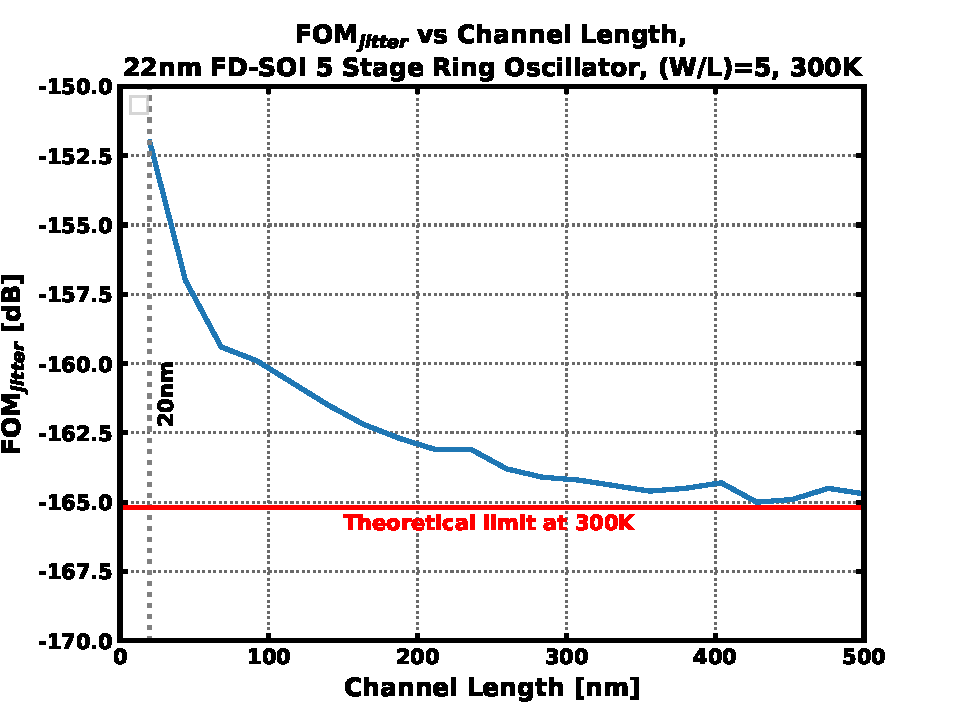
\includegraphics[width=1\textwidth, angle=0]{./figs/design/22fdx_rosc_fom_}
		        \caption{ }
		        \label{fig:rosc_fom}
		    \end{subfigure}%
		    \begin{subfigure}{0.5\textwidth}
		        \centering
		        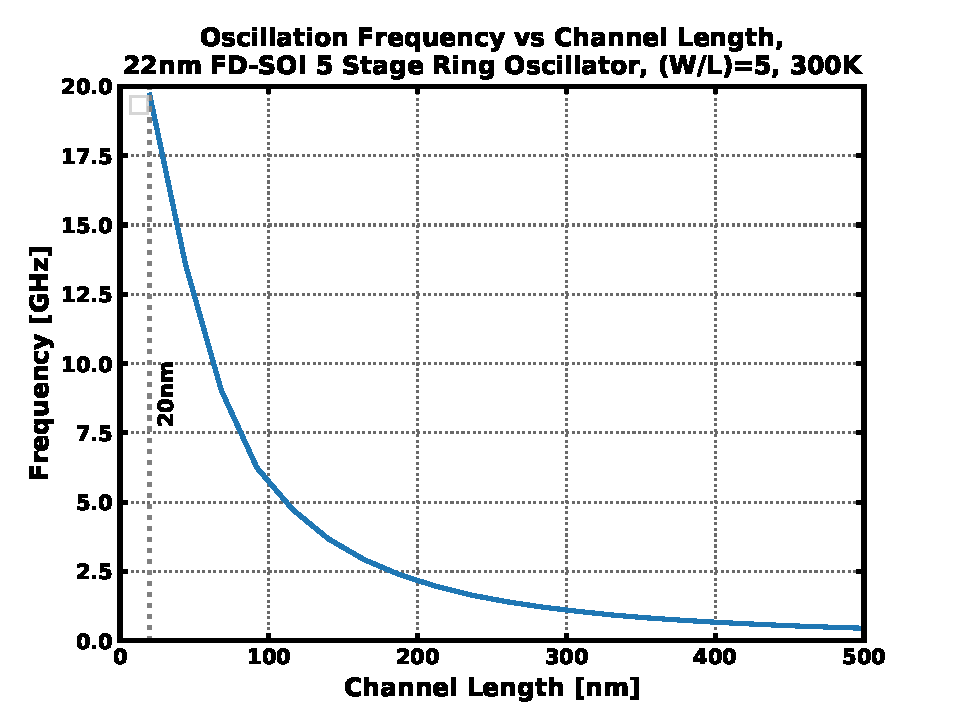
\includegraphics[width=1\textwidth, angle=0]{./figs/design/22fdx_rosc_freq}
		        \caption{ }
		        \label{fig:rosc_freq}
		    \end{subfigure}
		    % \caption{x.}
		    \label{fig:rosc_groupa}
		    \caption{22nm process ring oscillator channel length sweep versus \textbf{(a)} FOM, \textbf{(b)} Oscillation frequency.}
		\end{figure} 	

		% \begin{figure}[htb!]
		%     \centering
		%     \begin{subfigure}{0.5\textwidth}
		%         \centering
		%         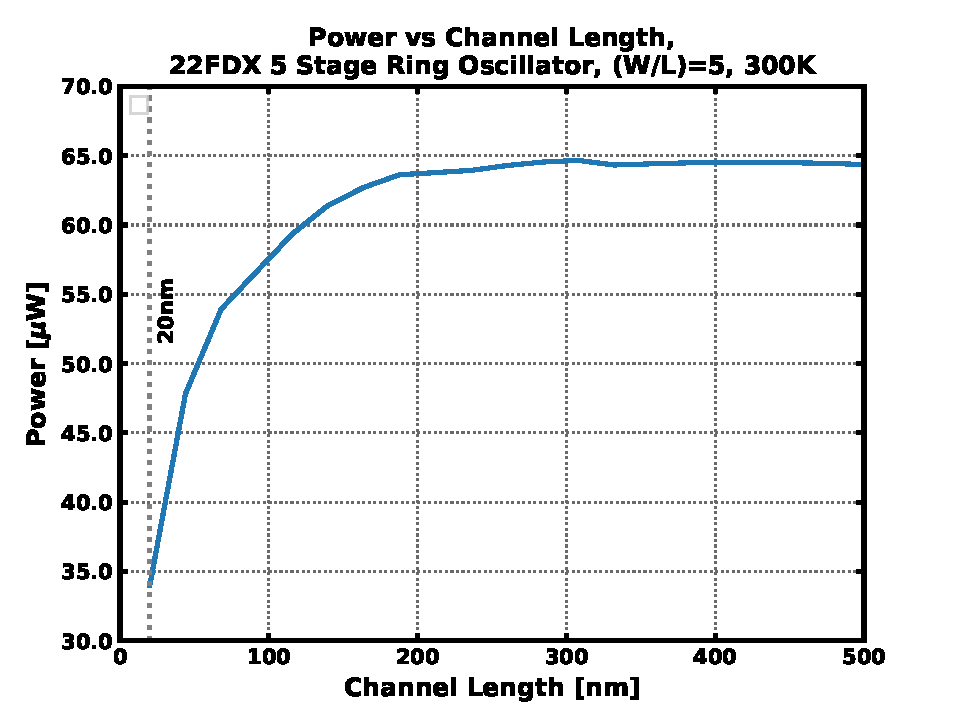
\includegraphics[width=1\textwidth, angle=0]{./figs/design/22fdx_rosc_power}
		%         \caption{ }
		%         \label{fig:rosc_power}
		%     \end{subfigure}%
		%     \begin{subfigure}{0.5\textwidth}
		%         \centering
		%         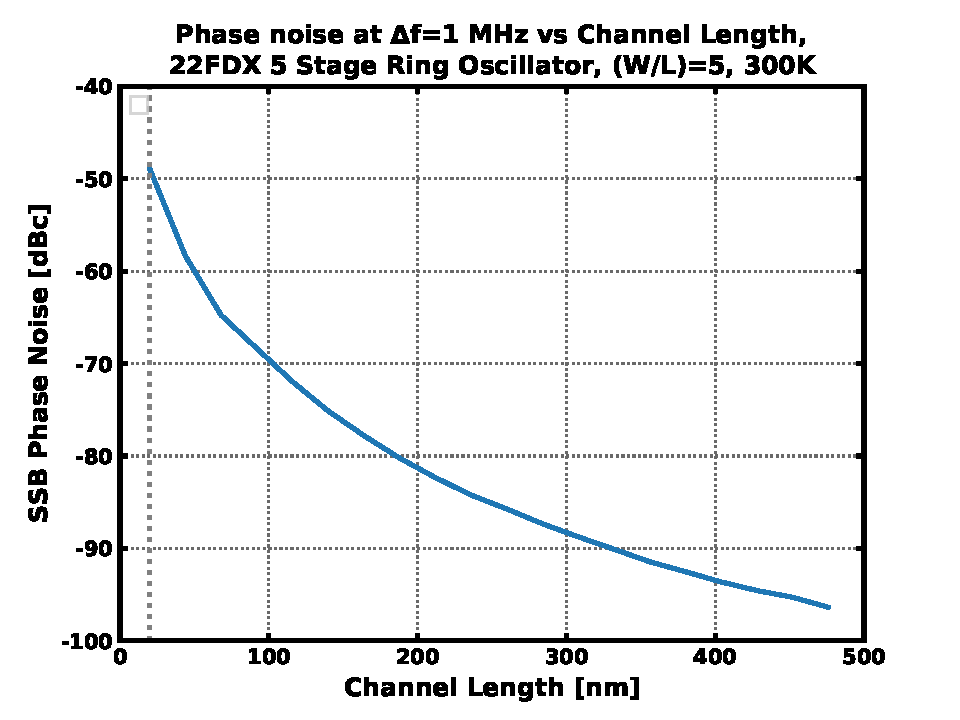
\includegraphics[width=1\textwidth, angle=0]{./figs/design/22fdx_rosc_pn_1mhz}
		%         \caption{ }
		%         \label{fig:rosc_pn_1m}
		%     \end{subfigure}
		%     % \caption{x.}
		%     \label{fig:rosc_groupb}
		%     \caption{22FDX ring oscillator channel length sweep versus \textbf{(a)} Power, \textbf{(b)} Phase noise at 1 MHz carrier offset (SSB).}
		% \end{figure} 

	\FloatBarrier





%%%%%%%%%%%%%%%%%%%%%%%%%%%%%%%%%%%%%%%%%%%%%%%%%%%%%%%%%%%%%%%%%%%%%%%%%%%



	\subsection{Ring Oscillator Frequency Model}\label{eq:freq_deriv}
		To analyze the effect of backgate tuning on a FD-SOI ring oscillator, a general mathematical model for CMOS ring oscillators will be developed first here. To begin, an approximate model for a CMOS inverter will first be considered. A typical model for delay in digital circuits is an RC circuit, where the MOSFET channels are approximated with an averaged conductance value $\langle g_{ch} \rangle$, and the output node is approximated to have a capacitance of C. With such a model, a ring oscillator is assumed to have waveforms that are decaying exponentials, with a time constant $\tau = \langle g_{ch} \rangle^{-1}C$. In context of the 3-stage ring oscillator of figure \ref{fig:rosc_rc}, figure \ref{fig:inv_model} demonstrates the described inverter model and the resulting input and output waveforms.

		\begin{figure}[htb!]
			\center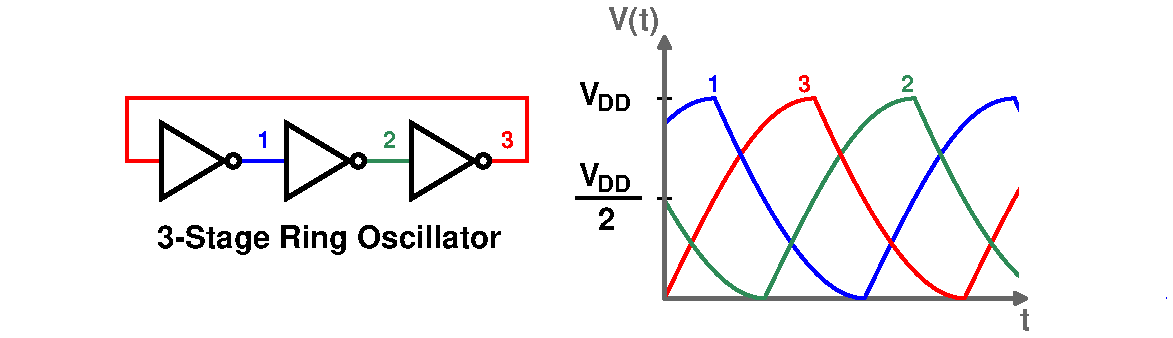
\includegraphics[width=0.8\linewidth, angle=0]{figs/theory/osc_waves}
			\caption{Model for ring oscillator.}
			\label{fig:rosc_rc}
		\end{figure}

		\begin{figure}[htb!]
	        \centering
	        \begin{subfigure}{.45\textwidth}
	            \centering
	            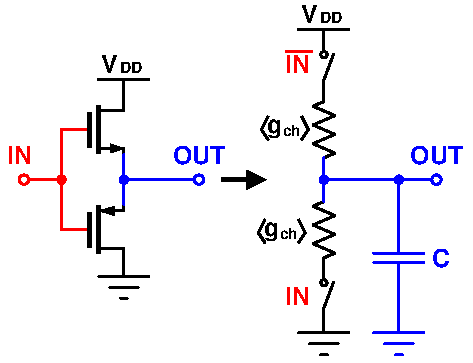
\includegraphics[width=\linewidth]{figs/design/inv_rc_model}
	            \caption{Inverter approximate model.}
	            \label{fig:inv_cir}
	        \end{subfigure}%
	        \begin{subfigure}{.5\textwidth}
	            \centering
	            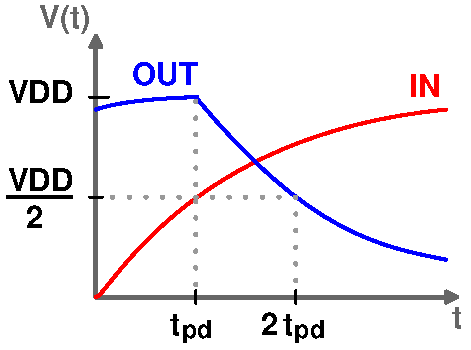
\includegraphics[width=0.8\linewidth]{figs/design/inv_waves}
	            \caption{Inverter waveforms in a ring oscillator.}
	            \label{fig:inv_wave}
	        \end{subfigure}
	        \caption{Approximate model for ring oscillator inverter delay cell.}
	        \label{fig:inv_model}
	    \end{figure}

		To calculate oscillation frequency of the ring oscillator from the RC model, several assumptions are made:
		\begin{itemize}
			\item The switching point $V_M$ of the inverters is $V_{DD}/2$, based on the assumption that the NMOS and PMOS are of equal strength.
			\item The output of the inverters will be decaying exponentials which start coincident with the passing of $V_M$ at the input.
			\item The propagation delay $t_{pd}$ for an inverter will be the time differential between the $V_M$ crossing points on the input and output.
			\item The oscillator frequency will be $f_{osc}$ = $1/2Nt_{pd}$, where N is the number of stages (i.e. defined by 2N propagation delays).
		\end{itemize}
			Given the falling edge inverter waveform equation in \ref{eq:inv_exp}, and observing that $t_{pd}$ occurs at the point where $V(t) = V_{DD}/2$, it is found that $t_{pd}$ = $\tau\ln(2)$. Finally, using the aforementioned assumptions, the equation for oscillator frequency is given in equation \ref{eq:ro_osc_freq}.

			\begin{equation}\label{eq:inv_exp}
			V(t) = V_{DD}\cdot e^{\frac{-t}{\tau}}\cdot u(t)
			\end{equation}

			\begin{equation}\label{eq:ro_osc_freq}
				f_{osc}^{-1} = 2Nt_{pd} = \frac{2\ln(2)NC}{\langle g_{ch}\rangle}
			\end{equation}


		\subsubsection{Finding $\langle g_{ch}\rangle$ and C}
			The node capacitance C is trivial to find based on the inverter gate capacitance and a lumped load capacitance term $C_L$:
			\begin{equation}
				C = C_{ox}\left ( W_N L_N + W_P L_N \right) + C_L
			\end{equation}
			The average channel conductance $\langle g_{ch} \rangle$ is more involved to find. To do so, several assumptions are made:
			\begin{itemize}
				\item L $>>$ L$_{min}$, so no velocity saturation, and therefore square law is applicable.
				\item NMOS and PMOS have equal $V_{TH}$ and transconductance.
				\item Output transitions occur with the active FET in saturation from the start of the transition until $t_{pd}$ after the start of the transition. This requires:
				\begin{itemize}
					\item $V_{DD}/4 < V_{TH} < V_{DD}/2$
				\end{itemize}
			\end{itemize}
			Following those assumptions, $\langle g_{ch} \rangle$ can be computed via integration within a period of $t_{pd}$ from the start of a transition:
			\begin{equation}
				\langle g_{ch} \rangle = \frac{1}{t_{pd}} \int_0^{t_{pd}}\frac{I_{out}(t)}{V_{out}(t)}dt
			\end{equation}
			$I_{out}$ is computed using the saturated MOSFET square law model and the assumption of exponential waveforms. An $I_{short}$ term is included to account for peak output current reduction from short-circuit conduction when both PMOS and NMOS devices are on.
			\begin{align}
				I_{out}(t) &= \frac{k_n}{2}\left(\frac{W}{L}\right)_n\left[\left(V_{in}(t) - V_{TH}\right)^2 \right]  - I_{short} \\
				&= \frac{k_n}{2}\left(\frac{W}{L}\right)_n \left[\left(V_{DD}\left(1-e^{-t/\tau}\right) - V_{TH}\right)^2 - \left(\frac{V_{DD}}{2} -V_{TH}\right)^2\right]
			\end{align}
			$k_n = \mu_nC_{ox}$, and with assumption of equal PMOS/NMOS, $k_n\left(\frac{W}{L}\right)_n=k_p\left(\frac{W}{L}\right)_p$. $V_{out}$ is simply a decaying exponential with a delay $t_{pd}$ versus the input:
			\begin{equation}
				V_{out}(t) = V_{DD}e^{-(t-t_{pd})/\tau}u(t)
			\end{equation}
			Now, computing the integral for $\langle g_{ch} \rangle$ yields:
			\begin{equation}
				\langle g_{ch} \rangle = \frac{1}{2}\mu_nC_{ox}\left(\frac{W}{L}\right)_n\left[V_{DD}\left(\frac{7}{8\ln2}-1\right)-V_{TH}\left(\frac{1}{\ln2}-1\right) \right]
			\end{equation}
			% As a simplification, $\alpha$ is defined as:
			% \begin{equation}
			% 	\alpha = \left[V_{DD}\left(\frac{7}{8\ln2}-1\right)-V_{TH}\left(\frac{1}{\ln2}-1\right) \right]
			% \end{equation}	
		
		% \subsubsection{Handling unequal NMOS/PMOS}
		% 	In the case of different threshold voltages for NMOS and PMOS:
		% 	\begin{equation}
		% 		f_{osc}^{-1} = N(t_{pdn} + t_{pdp}) = \ln(2)NC\left(\frac{1}{\langle g_{ch}\rangle_n} + \frac{1}{\langle g_{ch}\rangle_p}\right) = \frac{2\ln(2)NC}{\langle g_{ch}\rangle'}
		% 	\end{equation}	
		% 	A modified $\langle g_{ch}\rangle'$ is defined:
		% 	\begin{align}
		% 		\langle g_{ch}\rangle' = 2\left(\frac{1}{\langle g_{ch}\rangle_n} + \frac{1}{\langle g_{ch}\rangle_p}\right)^{-1} = 2\frac{\langle g_{ch}\rangle_n \langle g_{ch}\rangle_p}{\langle g_{ch}\rangle_n + \langle g_{ch}\rangle_p}
		% 		= 2\frac{\frac{1}{2}\mu_nC_{ox}\left(\frac{W}{L}\right)_n \alpha_n\frac{1}{2}\mu_pC_{ox}\left(\frac{W}{L}\right)_p \alpha_p}{\frac{1}{2}\mu_nC_{ox}\left(\frac{W}{L}\right)_n\alpha_n + \frac{1}{2}\mu_pC_{ox}\left(\frac{W}{L}\right)_p\alpha_p}
		% 	\end{align}	
		% 	This is somewhat unmanagable, however enforcing $\mu_nC_{ox}\left(\frac{W}{L}\right)_n = \mu_pC_{ox}\left(\frac{W}{L}\right)_p$ for $V_M$ to equal $V_{DD}/2$ gives:
		% 	\begin{align}
		% 		\langle g_{ch}\rangle' = \frac{1}{2}\mu_nC_{ox}\left(\frac{W}{L}\right)_n\frac{2 \alpha_n\alpha_p}{\alpha_n + \alpha_p} = \frac{1}{2}\mu_nC_{ox}\left(\frac{W}{L}\right)_n \alpha'
		% 	\end{align}	
		% 	Thus $\alpha_n$ and $\alpha_p$ are found for the according threshold voltages and then $\langle g_{ch}\rangle$ can be found.
		% 	\begin{equation}
		% 		\alpha' =  \frac{2 \alpha_n\alpha_p}{\alpha_n + \alpha_p}
		% 	\end{equation}

		\subsubsection{Oscillator Frequency and Power}
			Solving for oscillator frequency:
			\begin{equation}\label{eq:osc_freq_w_l}
				f_{osc} = \frac{\mu_nC_{ox}}{4\ln2NC}\left(\frac{W}{L}\right)_n\left[V_{DD}\left(\frac{7}{8\ln2}-1\right)-V_{TH}\left(\frac{1}{\ln2}-1\right) \right]
			\end{equation}
			If gate capacitance is the dominant load component, and PMOS/NMOS are equal sized such that $C=2WLC_{ox}$:
			\begin{equation}
				f_{osc} = \frac{\mu_n}{8\ln2N}\cdot\frac{1}{L^2}\left[V_{DD}\left(\frac{7}{8\ln2}-1\right)-V_{TH}\left(\frac{1}{\ln2}-1\right) \right]
			\end{equation}
			Power can also be calculated, knowing in digital circuits $P = fC_{\Sigma}V_{DD}^2$, where $C_{\Sigma}$ is the total capacitance of the active nodes. Thus:
			\begin{equation}\label{eq:osc_pow_consumption}
				P_{osc} = Nf_{osc}CV_{DD}^2 = \frac{\mu_nC_{ox}}{4\ln2}\left(\frac{W}{L}\right)_n\left[V_{DD}\left(\frac{7}{8\ln2}-1\right)-V_{TH}\left(\frac{1}{\ln2}-1\right) \right]
			\end{equation}
			It should be noted that the power consumption is proportional to FET aspect ratio (W/L), regardless of the load or frequency.

	\subsubsection{Ring Oscillator Backgate Frequency Tuning}
		Using the basic expressions for ring oscillator frequency, the frequency characteristics under backgate biasing can be found. In FD-SOI, the threshold voltage of a FET varies with linear dependence on the applied back gate bias $V_{BS}$ (relative to the source). Given the body effect coefficient of a process, $\gamma$, $V_{TH}$ is:
		\begin{equation}
			V_{TH} = V_{t0} - \gamma V_{BS}
		\end{equation}
		Using this in the ring oscillator frequency equation:
		\begin{equation}
			f_{osc} = \frac{\mu_nC_{ox}}{4\ln2NC}\left(\frac{W}{L}\right)_n\left[V_{DD}\left(\frac{7}{8\ln2}-1\right)-V_{t0}\left(\frac{1}{\ln2}-1\right) + \gamma V_{BS}\left(\frac{1}{\ln2}-1\right) \right]
		\end{equation}
		Equivalently, $f_{osc} = f_{0,osc} + \Delta f_{osc}(V_{BS})$, provided $f_{0,osc}$ is the frequency with no backgate bias where. Thus it is found that:
		\begin{equation}\label{eq:kvco_}
			\Delta f_{osc}(V_{BS}) = \gamma V_{BS}\frac{\mu_nC_{ox}}{4\ln2NC}\left(\frac{W}{L}\right)_n\left[\frac{1}{\ln2}-1\right] = K_{VCO}
		\end{equation}	

		The important finding here is that the change in oscillator frequency is linear with backgate voltage, that is $\Delta f_{osc} \propto V_{BS}$. The expression of \ref{eq:kvco_} also happens to to be the oscillator VCO gain, $K_{VCO}$. Given the wide voltage range that FD-SOI backgates may be biased to, this implies that a highly linear VCO with wide input range may be implemented with backgate tuning. If the backgate voltage is constrained in the range [0, $V_{DD}$], the center frequency $f_c$ of such a VCO is then:
		\begin{equation}
			f_{c} = \frac{\mu_nC_{ox}}{4\ln2NC}\left(\frac{W}{L}\right)_n\left[V_{DD}\left(\frac{7}{8\ln2}-1+\frac{\gamma}{2\ln2}-\frac{\gamma}{2}\right)-V_{t0}\left(\frac{1}{\ln2}-1\right)\right]
		\end{equation}
		Correspondingly, the tuning range with $V_{BS} \in$ [0, $V_{DD}$] is:
		\begin{equation}\label{eq:tuning_range}
			\Delta f = \gamma V_{DD}\frac{\mu_nC_{ox}}{4\ln2NC}\left(\frac{W}{L}\right)_n\left[\frac{1}{\ln2}-1\right]
		\end{equation}
		Finally, the fractional tuning range of the oscillator found to be that of equation \ref{eq:frac_range}. Notice that this is only a function of supply voltage $V_{DD}$, nominal threshold voltage $V_{t0}$ and body effect coefficient $\gamma$.
		\begin{equation}\label{eq:frac_range}
			\frac{\Delta f}{f_c} = \frac{\gamma V_{DD}\left( 1-\ln2 \right)}{V_{DD}\left(\frac{7}{8}-\ln2+\frac{\gamma}{2}-\frac{\gamma}{2}\ln2\right)-V_{t0}\left(1-\ln2\right)}
		\end{equation}	
		If a N-bit DAC is used to control the oscillator, the resulting DCO gain is therefore:
		\begin{equation}
			K_{DCO} = \frac{\Delta f}{2^{N_{DAC}}} = \frac{f_c}{2^{N_{DAC}}}\cdot\frac{\gamma V_{DD}\left( 1-\ln2 \right)}{V_{DD}\left(\frac{7}{8}-\ln2+\frac{\gamma}{2}-\frac{\gamma}{2}\ln2\right)-V_{t0}\left(1-\ln2\right)}
		\end{equation}	

	% \subsubsection{DCO Gain Uncertainty}
	% 	The DCO gain $K_{DCO}$ is used in setting the loop filter coefficients, so the uncertainty of the DCO gain is of interest to allow for statistical analysis of the PLL across process variation. The uncertainty of $K_{DCO}$ (normalized with nominal $K_{DCO}$ value) as a function of $V_{DD}$, $V_{t0}$ and $\gamma$ is:
	% 	\begin{equation}
	% 		\sigma_{KDCO} = \sqrt{\left(\frac{\partial K_{DCO}}{\partial V_{DD}}\cdot\frac{\sigma_{VDD}}{K_{DCO}} \right)^2 + \left(\frac{\partial K_{DCO}}{\partial V_{t0}}\cdot\frac{\sigma_{Vt0}}{K_{DCO}} \right)^2 + \left(\frac{\partial K_{DCO}}{\partial \gamma}\cdot\frac{\sigma_\gamma}{K_{DCO}} \right)^2}
	% 	\end{equation}

	% 	\begin{align}
	% 		\frac{\partial K_{DCO}}{\partial V_{DD}} &= \frac{f_c}{2^{N_{DAC}+1}}\cdot\frac{-\gamma V_{t0}(1-\ln2)^2}{\left[ V_{DD}\left(\frac{7}{8}-\ln2+\frac{\gamma}{2}-\frac{\gamma}{2}\ln2\right)-V_{t0}\left(1-\ln2\right) \right]^2}\\
	% 		\frac{\partial K_{DCO}}{\partial V_{t0}} &= \frac{f_c}{2^{N_{DAC}+1}}\cdot\frac{\gamma V_{DD}(1-\ln2)^2}{\left[ V_{DD}\left(\frac{7}{8}-\ln2+\frac{\gamma}{2}-\frac{\gamma}{2}\ln2\right)-V_{t0}\left(1-\ln2\right) \right]^2}\\
	% 		\frac{\partial K_{DCO}}{\partial \gamma} &= \frac{f_c}{2^{N_{DAC}+1}}\cdot\frac{V_{DD}\cdot(1-\ln2) \left[ V_{DD}\left(\frac{7}{8}-\ln2\right)-V_{t0}\left(1-\ln2\right) \right]}{\left[ V_{DD}\left(\frac{7}{8}-\ln2+\frac{\gamma}{2}-\frac{\gamma}{2}\ln2\right)-V_{t0}\left(1-\ln2\right) \right]^2}
	% 	\end{align}
	% 	Simplified:
	% 	\begin{multline}
	% 		\sigma_{KDCO} = \frac{1}{\gamma V_{DD} \left[ V_{DD}\left(\frac{7}{8}-\ln2+\frac{\gamma}{2}-\frac{\gamma}{2}\ln2\right)-V_{t0}\left(1-\ln2\right) \right]}\cdot\\ \sqrt{\left(\gamma V_{t0} (1-\ln2)\sigma_{VDD} \right)^2 + \left(\gamma V_{DD} (1-\ln2)\sigma_{Vt0} \right)^2 + \left( V_{DD}\left[ V_{DD}\left(\frac{7}{8}-\ln2\right)-V_{t0}\left(1-\ln2\right) \right]\sigma_{\gamma} \right)^2 }
	% 	\end{multline}	

		% \hl{Motivate selection of fine backgate tuning and supply coarse tuning (as future extension?). I.e. what is df/dVdd vs df/dVbg?}
		% \hl{\textbf{TODO} - extract $\gamma$, $V_{t0}$ variance for FETs in process kit, place in results?}

		\subsubsection{Backgate-controlled Ring Oscillator Sensitivity Analysis}\label{sec:sens_analysis}
		The frequency tuning sensitivity of the ring oscillator for supply and backgate voltages will be compared. First the following is defined, seeing that the derived equations for oscillator frequency versus backgate bias and supply voltage are linear.
		\begin{equation}
			f_{osc}(V_{DD}+\Delta V_{DD}) = f_{osc}(V_{DD}) + f_{osc}(\Delta V_{DD})
		\end{equation}
		\begin{equation}
			f_{osc}(V_{DD}) = f_0
		\end{equation}
		\begin{equation}
			f_{osc}(\Delta V_{DD}) = \Delta f
		\end{equation}

		In the case of supply voltage tuning, the change as a proportion of nominal frequency per voltage of applied extra bias is (evaluated at zero back-gate bias):
		\begin{equation}
			S^{f_{osc}}_{V_{DD}} = \frac{\Delta f}{f_0}\cdot\frac{1}{\Delta V_{DD}}  = \frac{\left(\frac{7}{8\ln2}-1\right)}{V_{DD}\left(\frac{7}{8\ln2}-1\right)-V_{t0}\left(\frac{1}{\ln2}-1\right)}
		\end{equation}
		With $V_{DD}$ = 0.8, $V_{t0}$ = 0.3 (approximately true for the FD-SOI devices of this work), it is expected 340\% change in frequency will result per extra volt of applied bias. Of course, this is linearized, and one does not expect to apply an extra 1V of supply bias to a 0.8V oscillator. Realistically, the supply can be tuned $\pm$ 10\%, which corresponds to a $\pm$27.2\% tuning range of the oscillator. Supply tuning stands as a viable coarse tuning mechanism for the oscillator, however, fine tuning is more limited due to difficulty in achieving a small resolution step (e.g 10 bits in $V_{DD}$ = 0.8V $\pm$10\% corresponds to 156 $\mu$V/LSB, and 26 m\%/LSB of frequency tuning).

		\par In the case of backgate tuning, the change (proportion) of frequency per volt of applied backgate bias is:
		\begin{equation}
			S^{f_{osc}}_{V_{BG}} = \frac{\Delta f}{f_0}\cdot\frac{1}{\Delta V_{BG}}  = \frac{\gamma \left(\frac{1}{\ln2}-1\right)}{V_{DD}\left(\frac{7}{8\ln2}-1\right)-V_{t0}\left(\frac{1}{\ln2}-1\right)}
		\end{equation}

		With $\gamma$ = 0.07, $V_{DD}$ = 0.8, $V_{t0}$ = 0.3, as is typical in the FD-SOI process in this work, it is expected a 29.5\% change in frequency will result per volt applied of backgate bias. This is much finer than achieved with supply voltage tuning. The ratio of frequency sensitivity to supply and backgate voltage tuning is:

		\begin{equation}
			\frac{S^{f_{osc}}_{V_{DD}}}{S^{f_{osc}}_{V_{BG}}} =  \frac{\frac{7}{8\ln2}-1}{\gamma \left(\frac{1}{\ln2}-1\right)}
		\end{equation}
		Under the aforementioned biasing conditions, it is expected that 8.4x finer control can be achieved with backgate tuning per unit of applied bias. The wide backgate voltage ranges allowed for with FD-SOI technology furthermore permit for design of a voltage-DAC based control scheme which will achieve far smaller frequency resolution than with supply voltage tuning. Therefore, motivated by these findings, the pursuit of a backgate tuned ring oscillator has been undertaken in this work.

		% \subsubsection{Capacitor-based coase tuning scheme}
		% It is observed that oscillator frequency of ring oscillator is capacitance dependent. Thus if a bank of quantized capacitances may be switched into the oscillator, coarse control of frequency can be implemented. Figure \ref{fig:rosc_tuning} demonstrates the effect of such a tuning scheme, for increasing capacitance settings C0-C3. Under such a scheme it is important to ensure that the frequency ranges acheived through backgate tuning overlap between successive capacitor settings to ensure continuity of frequencies accessible by the oscillator. 
		% \FloatBarrier
		% \begin{figure}[htb!]
		% 	\center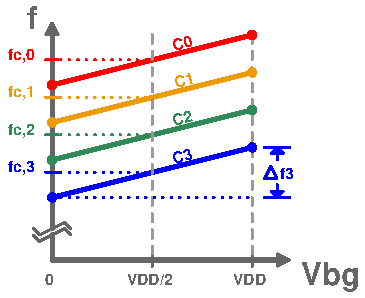
\includegraphics[width=0.4\linewidth, angle=0]{figs/backgate_rosc_tuning2.pdf}
		% 	\caption{Backgate-tuned ring oscillator with coarse tuning capacitor bank.}
		% 	\label{fig:rosc_tuning}
		% \end{figure}




%%%%%%%%%%%%%%%%%%%%%%%%%%%%%%%
		
		\FloatBarrier\pagebreak
		\subsection{Pseudodifferential Backgate-Coupled Inverter Delay Cell}\label{sec:pd_inv}
		To utilize backgate tuning for frequency control, a suitable delay cell design must be devised. Accordingly, the delay topology used in this work has been derived from the FD-SOI pseudodifferential backgate coupled inverter delay cell of \cite{Jacquemod2019}, shown in figure \ref{fig:bg_inv_jacqu}. This inverter uses two single ended FD-SOI inverters, with the backgates of the transistors in a given inverter connected together. This is implemented with a common well structure below the two transistors of each inverter. Nominally, to avoid forward biasing of the well-substrate diodes, a N-doped well or a triple well is used, with well potentials constrained to be $\geq$ 0. The result of this well configuration and the FD-SOI BOX layer is that the backgate terminals of the PMOS and NMOS may be tuned in tandem across a wide positive voltage range. This is not possible in bulk technology. In the FD-SOI process used in this work, such well configurations allow biasing from 0 to +2V, which is inclusive of the full rail-to-rail range of a circuit supplied with $V_{DD}$ = 0.8V, as in this work. Thus, in figure \ref{fig:bg_inv_jacqu}, when the two FD-SOI sub-cells inverter cells connected with the shown cross-coupled output and backgate configuration, safe well biasing is achieved. The backgate cross-coupled configuration has the effect of inducing differential behavior in the circuit, as positive feedback is introduced. It should be noted that the cell of figure \ref{fig:bg_inv_jacqu} does not employ backgate-based tuning to tune cell delay. This work proposes a modification to the topology which implements both backgate differential coupling and backgate frequency (delay) tuning.

		\begin{figure}[htb!]
		        \centering
		        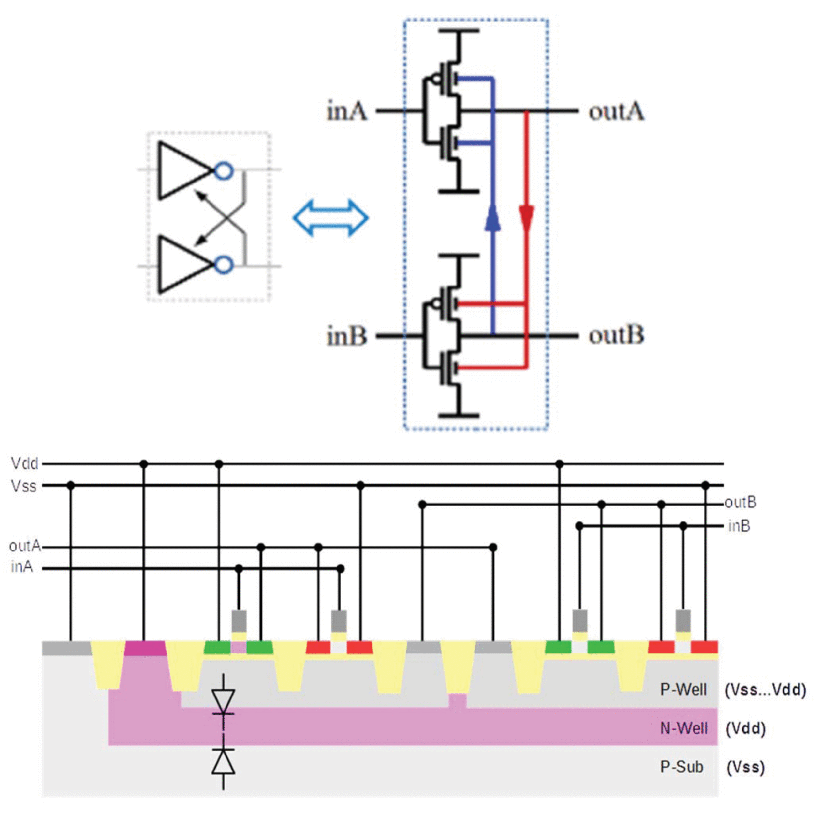
\includegraphics[width=0.58\textwidth, angle=0]{./figs/design/jacqu2-1-large.png}
		    \caption{FD-SOI backgate-coupled inverter topology \cite{Jacquemod2019}.}
		    \label{fig:bg_inv_jacqu}
		\end{figure}	

		The emergence of differential behavior in this delay cell can be understood through circuit analysis. First, the common backgate inverter cell (figure \ref{fig:fig_10a}) is converted to a linearized model, for an arbitrary bias point, in figure \ref{fig:fig_10b}. A simplification of the linearized model is arrived at by lumping terms together, giving figure \ref{fig:fig_10c}. Using the linearized model of figure \ref{fig:fig_10c}, a linearized version of the pseudodifferential inverter circuit is then arrived at in figures \ref{fig:pseudodiff_cir} and \ref{fig:pseudodiff_linearized}. It is observed that the backgate transconductors (labeled as $-G_{mb}$) in figure \ref{fig:pseudodiff_linearized} couple the two outputs with a positive feedback loop. Therefore, any differential components generated via the feed forward terms $-G_m R_o v_{in}$ and $-G_m R_o v_{ip}$ will be positively amplified by the cross coupling. Elementary circuit analysis for differential gain of the linear circuit in figure \ref{fig:pseudodiff_linearized} leads to the expression in equation \ref{eq:pd_dm_gain}.

			\begin{figure}[htb!]
			    \centering
			    \begin{subfigure}{0.25\textwidth}
			        \centering
			        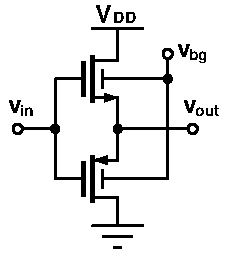
\includegraphics[width=1\textwidth, angle=0]{./figs/design/fig_10a_}
			        \caption{ }
			        \label{fig:fig_10a}
			    \end{subfigure}%
			    \begin{subfigure}{0.33\textwidth}
			        \centering
			        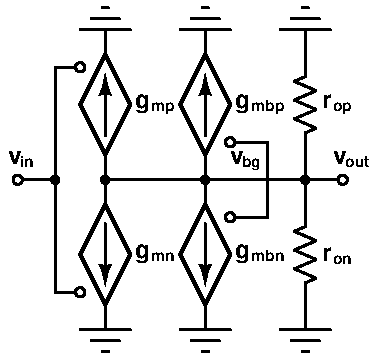
\includegraphics[width=1\textwidth, angle=0]{./figs/design/fig_10b}
			        \caption{ }
			        \label{fig:fig_10b}
			    \end{subfigure}
			    \begin{subfigure}{0.33\textwidth}
			        \centering
			        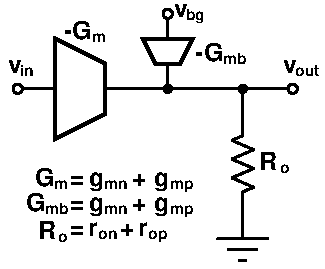
\includegraphics[width=1\textwidth, angle=0]{./figs/design/fig_10c}
			        \caption{ }
			        \label{fig:fig_10c}
			    \end{subfigure}
			    % \caption{x.}
			    \caption{\textbf{(a)} Common backgate inverter, \textbf{(b)} Linearized circuit, \textbf{(c)} Simplified linearized model.}
			    \label{fig:bg_inv_model}
			\end{figure} 

			\begin{figure}[htb!]
			    \centering
			    \begin{subfigure}{0.25\textwidth}
			        \centering
			        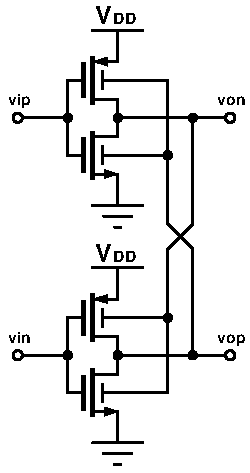
\includegraphics[width=1\textwidth, angle=0]{./figs/design/pseudodiff_bw}
			        \caption{ }
			        \label{fig:pseudodiff_cir}
			    \end{subfigure}%
			    \hspace{5em}
			    \begin{subfigure}{0.35\textwidth}
			        \centering
			        \includegraphics[width=1\textwidth, angle=0]{./figs/design/pseudodiff_buff_linear}
			        \caption{ }
			        \label{fig:pseudodiff_linearized}
			    \end{subfigure}
			    % \caption{x.}
			    \caption{\textbf{(a)} Pseudodifferential backgate-coupled inverter circuit, \textbf{(b)} Linearized circuit.}
			    \label{fig:pd_cir_inv_model}
			\end{figure} 

			\begin{equation}\label{eq:pd_dm_gain}
				A_{DM} = \frac{G_mR_o + G_{mb}^2R_o^2}{1 - G_{mb}^2R_o^2}
			\end{equation}
			Using the relation $G_{mb} = \gamma G_{m}$ found in equation \ref{eq:gm_gmb_relation}, equation \ref{eq:pd_dm_gain} can be simplified to equation \ref{eq:pd_dm_gain2} (this is assuming PMOS and NMOS have approximately equal $\gamma$). In the special case where $\gamma G_mR_o \approx 1$, the differential gain of the delay cell can be very high, implying the pseudodifferential backgate coupling can be very effective at inducing differential behavior. A major advantage of this topology is that it is implemented using only two inverters, unlike typical differential pair circuits which rely on current biasing to achieve differential behavior. The removal of the need for current biasing reduces power consumption, as no reference current generation is required. Circuit noise is also reduced due to fewer total transistors generating noise in the circuit.
			\begin{equation}\label{eq:pd_dm_gain2}
				A_{DM} = \frac{G_mR_o }{1 - \gamma G_mR_o }
			\end{equation}
			For the sake of completeness, the common mode gain of the circuit has also been determined through circuit analysis, given in equation \ref{eq:pd_cm_gain}.
			\begin{equation}\label{eq:pd_cm_gain}
				A_{CM} = \frac{G_mR_o }{1 + \gamma G_mR_o }
			\end{equation}

%%%%%%%%%%%%%%%%%%%%%%%%%%%%%%%%%%%%%%%%%%%%%%%%%%%%%%%%%%%%%%%%%%%%%%%%%%%



			\FloatBarrier
			\subsubsection{Tunable Frequency Backgate-Coupled Pseudodifferential Delay Cell}
			To implement the backgate-coupled pseudo-differential inverter delay cell topology with backgate tuning, two candidate topologies have been devised. The first is the parallel configured topology of figure \ref{fig:parallel_delay_cell}, and the second is a telescopic configuration, shown in figure \ref{fig:telescopic_delay_cell}. Tuning of the delay cells is done in accordance with figure \ref{fig:bg_tuning_scheme}, where the backgate voltages \textit{vbgp} and \textit{vbgn} change in a complementary fashion. Tuning for increased frequency results in greater $|V_{BS}|$ biasing for both PMOS and NMOS, such that the threshold voltage in both devices decreases, modulating the channel conductances to be higher and accordingly increasing frequency. These cells were devised with a priority to maintain overall symmetry, specifically in regards to rise and fall time behavior. Hajimiri's highly cited paper \cite{Hajimiri1998} on the effect of impulse injection on oscillator edges finds that it is favorable for an oscillator to have as symmetric rise and fall time in terms of phase noise. Specifically, it was found that higher symmetry of waveform in terms of rise and fall behavior results in a lower corner frequency for flicker noise, thus improving low frequency phase noise components of an oscillator. 

			\begin{figure}[htb!]
			    \centering
			    \begin{subfigure}{0.5\textwidth}
			        \centering
			        \includegraphics[width=1\textwidth, angle=0]{./figs/design/parallel_delay_cell2}
			        \caption{ }
			        \label{fig:parallel_delay_cell}
			    \end{subfigure}%
			    \begin{subfigure}{0.5\textwidth}
			        \centering
			        \includegraphics[height=0.5\textheight, angle=0]{./figs/design/tele_delay_cell2}
			        \caption{ }
			        \label{fig:telescopic_delay_cell}
			    \end{subfigure}
			    % \caption{x.}
			    \label{fig:tunable_delay_cells}
			    \caption{Backgate tunable backgate-coupled pseudodifferential delay cell in \textbf{(a)} Parallel, and \textbf{(b)} Telescopic implementations.}
			\end{figure} 

			\begin{figure}[htb!]
			    \centering
			    \includegraphics[width=0.33\textwidth, angle=0]{./figs/design/tuning}
			    \caption{Complementary tuning of backgate voltages to achieve frequency tuning.}
			    \label{fig:bg_tuning_scheme}
			\end{figure}

			The parallel configured topology employs a backgate-coupled pseudo-differential inverter in parallel with a second set of inverters, which the backgate voltages are set externally to control the oscillator frequency. The delay cell operates through superposition position of current, by connecting the inverters in parallel, their individual effects are combined to result in both frequency tuning and differential operation. The frequency gain of this delay cell is controlled by setting a ratio of the device widths utilized in the cross-coupled inverter to the widths of the frequency tuning inverters. If this ratio is defined as R = W$_{1x}$/W$_{3x}$ = W$_{2x}$/W$_{4x}$, the VCO gain is defined in equation \ref{eq:parallel_kvco}. In a simulation case with the 22nm FD-SOI technology of this work using LVTNMOS + RVTPMOS devices, a nominal (W/L) = 200nm/150 nm for all devices, $V_{DD}$ = 0.8, and R = 1, a fractional tuning range of 14.9\% was observed in the ring oscillator. Changing R = 2 results in 10.7\% fractional tuning range. These are consistent with the predicted equation, and suggest a maximum fractional tuning range of 29.8\%-32.1\% for this backgate controlled oscillator (where R = 0). Based on the theoretical oscillator fractional frequency tuning range in equation \ref{eq:frac_range}, and the extracted body effect coefficient parameters given in appendix \ref{sec:fet_extracted_data} for the 22nm FD-SOI process, where $\gamma \approx$ 0.075 and $V_{t0} \approx$ 0.3, it is found that theoretically the maximum tuning range should be 29.4\%, which agrees closely with the simulation results. This suggests validity of the developed oscillator theory.

			\begin{equation}\label{eq:parallel_kvco}
				K_{VCO,parallel}^{'} = \frac{K_{VCO}}{R + 1}
			\end{equation}

			The telescopic topology is comprised of two sub-inverters each with a telescopic stack of four transistors. The header and footer transistor backgates are connected to external control voltages to adjust the frequency. Modulating the control voltages will modulate the conductance of the header and footer devices, resulting in a current-starving like behavior that tunes the oscillator frequency. The inner pair of transistors in each sub-inverter are configured with a common backgate, which are cross-coupled with the output of the other respective sub-inverter, to induce differential operation in the same manner as the basic backgate-coupled pseudo-differential inverter delay cell. Frequency gain of the cell is controlled via setting the ratio of the inner transistors to the header and footer transistors. Due to the telescopic arrangement, a simple argument of current superposition as in the parallel case can not be made. Also, the model assumptions made in the backgate-controlled oscillator theory of section \ref{eq:freq_deriv} are not necessarily valid, as the FET operating regime of the telescopic devices cannot be guaranteed to be in saturation during the delay cell propagation period. Rather than a full circuit analysis of this topology, an approximate result backed by simulated observations has been devised. If a ratio R is defined as R = W$_{1x}$/W$_{2x}$ = W$_{4x}$/W$_{3x}$, it was determined via simulation that the oscillator frequency gain is reduced by 1/R for R near unity. Combining the two aforementioned observations results in equation \ref{eq:series_kvco}. In a simulation case with FD-SOI technology where LVTNMOS + RVTPMOS devices, a nominal (W/L) = 400nm/150 nm for all devices, and R = 1, a fractional tuning range of 10\% was observed in the ring oscillator. Changing R = 2 resulted in a 4.8\% fractional tuning range.

			\begin{equation}\label{eq:series_kvco}
				K_{VCO, telescopic}^{'} = \frac{K_{VCO}}{R}
			\end{equation}

			These two topologies present different trade offs between frequency and achievable power. Inspecting equation \ref{eq:osc_pow_consumption}, it is seen that oscillator power consumption is proportional to device (W/L) used in the delay cells. For low power, low effective (W/L) is desirable. In the case of the parallel delay stage, an effective (W/L)$_{parallel}^{'}$ is arrived at by adding the device (W/L)'s of the cross-coupled and frequency tuning sub-inverters, yielding (W/L)$_{parallel}^{'}$ = (1+R)(W/L). In the telescopical case, assuming R=1, it is observed that to two FETs with size (W/L) cascaded have an effective (W/L)$_{tele}^{'}$ = 0.5(W/L). It is expected that minimum power attainable is achieved by utilizing the smallest available devices size in a technology, that is (W$_{min}$/L$_{min}$), with R=1. Comparing the telescopic and parallel cases, it is seen that (W/L)$_{parallel}^{'}$/(W/L)$_{tele}^{'}$ = 4, implying that the power consumption of the parallel stage can be presumed to be four times that of the series design with equal device sizes. In the case of this work, scaling of power is very important, and it has been found that the parallel topology was unable to achieve small enough $K_{VCO}$ needed in this work with satisfactory power consumption. This is due to the need to increase R to reduce $K_{VCO,parallel}^{'}$, which correspondingly increases power due to greater effective inverter width. Thus, a telescopic topology has been pursued in this work.

			\begin{figure}[htb!]
			        \centering
			        \includegraphics[height=0.5\textheight, angle=0]{./figs/design/delay_cell_pd_inv}
			    \caption{Pseudo-differential backgate-coupled inverter delay cell with fine and medium backgate-based tuning.}
			    \label{fig:delay_cell_pd_inv}
			\end{figure}


		% {\color{white}.}\FloatBarrier
		% \subsubsection{Final Delay Circuit}
	The final delay cell inverter topology employed in this work is shown in figure \ref{fig:delay_cell_pd_inv}, which is the previous telescopic topology with a modification to enable simultaneous fine and coarse tuning ranges. This modification is achieved with the addition of a second transistor to each the header and footer of the telescopic stage. Transistors M$_{1x}$ and M$_{5x}$ implement medium granularity tuning, and transistors M$_{2x}$ and M$_{6x}$ implement fine granularity tuning. Defining R = W$_{1x}$/W$_{2x}$ = W$_{5x}$/W$_{6x} >$ 1, tuning the parameter R can be utilized to provide different tuning gains for the two ranges with respect to the applied backgate biases. This topology has been arrived at due to the finding that with the DACs implemented in this work, it was not possible to simultaneously achieve a wide tuning range with satisfactorily small $K_{DCO}$ resolution with a single set of backgates. For sizing of devices, it is recommended to select a channel length selected based on the findings for FOM$_{jitter}$ versus channel length in section \ref{sec:chan_len_22fdx}, picking the longest channel length possible. Then, the width of all devices (set equal) should be varied until the target power is achieved. Finally, the header and footer device widths should be varied until satisfactory $K_{VCO}$ values are found for the delay cell topology. Achieving design goals with this topology may require several iterations with layout.

	{\color{white}.}\FloatBarrier
	\subsection{Oscillator Implementation}
	\subsubsection{Number of Ring Oscillator Stages}\label{sec:num_stages}
	In the process of simulating the proposed delay cell in the 22nm FD-SOI technology, it has been determined that a two stage differential ring oscillator, generating in-phase and quadrature phase signals, will not oscillate. With a delay stage propagation time of $t_{pd}$, the cycle period is $1/f_{osc} = 2Nt_{pd}$, where in this case the number of stages $N$ = 2. Every node is expected to switch two times per cycle, therefore it is determined that the switching period of a given node is equal to $2t_{pd}$. Previously, it has been determined that the propagation delay for the RC dominated ring oscillator is $\ln(2)\tau$, resulting in a switching period of $2\ln(2)\tau$. If the oscillator swings from 0 to $V_{DD}$ with exponential dependence, in a time period of $2\ln(2)\tau$, a change of 0.75$V_{DD}$ is expected at the oscillator nodes. This implies that a two stage ring oscillator will not fully saturate to the rails, and therefore results in an extinction of oscillation as seen via simulation. Originally, it was planned to implement a two-stage quadrature VCO at 2.448 GHz, however due to the infeasibility of this, alternative configurations were attempted. First was a 4-stage oscillator at 2.448 GHz, however, it was seen that it was not possible to achieve the desired power and phase noise requirements with the proposed telescopic backgate-coupled delay cell in the 22nm FD-SOI process used. Thus, another alternative, being a subharmonic oscillator operating at 1/3 of 2.448 GHz was considered. This was implemented as a 6-stage differential ring oscillator, as shown in figure \ref{fig:basic_6stg_ro}, which oscillates at 816 MHz. With 6 differential stages, 12 oscillator phases are created, and it is possible to derive a quadrature 2.448 GHz sampling clock by combining with digital logic the different 816 MHz oscillator phases, as shown in figure \ref{fig:ro_phases}. With this topology, it was found to be feasible to implement a 816 MHz, 6-stage oscillator in 22nm FD-SOI that meets power and phase noise requirements defined for the design.


			\begin{figure}[htb!]
			        \centering
			        \includegraphics[width=0.8\textwidth, angle=0]{./figs/design/ro_6st_simple}
			    \caption{Basic differential ring oscillator circuit.}
			    \label{fig:basic_6stg_ro}
			\end{figure}



			\begin{figure}[htb!]
			        \centering
			        \includegraphics[width=1.0\textwidth, angle=0]{./figs/design/ro_12ph_quad}
			    \caption{Third subharmonic to quadrature full rate conversion.}
			    \label{fig:ro_phases}
			\end{figure}

%%%%%%%%%%%%%%%%%%%%%%%%%%%%%%%%%%%%%%%%%%%%%%%%%%%%%%
	% {\color{white}.}
		\FloatBarrier%\pagebreak
	\subsubsection{Final Oscillator Circuit}
	\FloatBarrier
	With a selection of the inverter topology and number of delay cells, the final oscillator circuit topology is described here. The oscillator is comprised of six basic delay cell elements shown in figure \ref{fig:delay_cell_circuit}, which contain (1) a backgate-coupled and tunable pseudodifferential inverter, (2) reset switches, and (3), an output buffer. A simplified symbol for the delay cell is shown in figure \ref{fig:delay_cell_symbol}, and the placement of the delay cells into a full ring oscillator is shown in figure \ref{fig:full_6sg_ro}. This delay cell was devised from the base inverter topology in order to fulfill several goals. The first goal is to be able to reset the oscillator to a known phase at start up, which is implemented via addition of switches at the output nodes which force the nodes to rail levels when a reset condition is asserted. This is such that when reset is de-asserted in tandem with a clock edge for the PLL, the initial edge of the oscillator sampled by a phase detector will be in sync with the clock, as shown in figure \ref{fig:dco_reset}. The second goal is to remove any effect of external noise and loading on the oscillator, for which a buffer has been added to each delay cell, that the external world connects to. This is discussed in section \ref{sec:buffer}. Table \ref{tab:dly_dev_size} contains the devices sizes used to implement the delay cell of figure \ref{fig:delay_cell_circuit}. The devices types selected for implementation are low voltage threshold NMOS (LVTNMOS) and regular voltage threshold PMOS (RVTPMOS) in the 22nm FD-SOI process. These are selected based on the discourse in appendices \ref{sec:fet_extracted_data} and \ref{sec:opt_wp_wn}, which show these devices are well matched in terms of body coefficient and allow for near unity ratio of W$_P$/W$_N$ for a V$_{DD}$/2 output crossing level.
	\vspace{-2em}
	\begin{figure}
		\begin{floatrow}
		\ffigbox{%
			\includegraphics[height=0.45\textheight, angle=0]{./figs/design/delay_cell_full2}
		}{%
			    \caption{Ring oscillator delay cell full circuit.}
			    \label{fig:delay_cell_circuit}
		}
		\capbtabbox{%
			\def\arraystretch{1.5}		
			\setlength\arrayrulewidth{0.75pt}
			\setlength{\tabcolsep}{1em} % for the horizontal padding
			\begin{tabular}{|c|c|}
				\hline 
				\rule[-1ex]{0pt}{2.5ex} \cellcolor{gray!40}\textbf{Device} & \cellcolor{gray!40}\textbf{(W/L)} \\ 
				\hline 
				\rule[-1ex]{0pt}{2.5ex} M$_{1x}$, M$_{5x}$ & 800n/40n\\ 
				\hline 
				\rule[-1ex]{0pt}{2.5ex} M$_{2x}$, M$_{6x}$ & 100n/40n\\ 
				\hline 
				\rule[-1ex]{0pt}{2.5ex} M$_{3x}$, M$_{4x}$ & 400n/40n\\ 
				\hline 
				\rule[-1ex]{0pt}{2.5ex} M$_{7x}$, M$_{8x}$ & 200n/20n\\ 
				\hline 
				\rule[-1ex]{0pt}{2.5ex} M$_{9,1}$, ..., M$_{9,n}$ & 100n/20n\\ 
				\hline 
				\rule[-1ex]{0pt}{2.5ex} M$_{10x}$, M$_{11x}$ & 200n/20n\\ 
				\hline 
				\rule[-1ex]{0pt}{2.5ex} C$_L$ & 200 aF\\ 
				\hline 
			\end{tabular} 
		}{%
			\caption{Delay Stage Device Sizes.}
			\label{tab:dly_dev_size}
		}
		\end{floatrow}
	\end{figure}




	\begin{figure}[htb!]
	    \centering
	    \begin{subfigure}{0.5\textwidth}
	        \centering
	        \includegraphics[width=1\textwidth, angle=0]{./figs/design/delay_cell_symbol_full2}
	        \caption{ }
	        \label{fig:delay_cell_symbol}
	    \end{subfigure}%
	    \begin{subfigure}{0.5\textwidth}
	        \centering
	        \includegraphics[width=1\textwidth, angle=0]{./figs/design/osc_reset}
	        \caption{ }
	        \label{fig:dco_reset}
	    \end{subfigure}
	    % \caption{x.}
	    \label{fig:vco_symbol_reset}
	    \caption{\textbf{(a)} Ring oscillator delay cell symbol, \textbf{(b)} Oscillator synchronous reset scheme.}
	\end{figure} 


	\begin{figure}
		\center%
		\includegraphics[width=1.5\textwidth, angle=90]{./figs/design/rosc_full_6stg2}
	    \caption{Ring oscillator full schematic.}
	    \label{fig:full_6sg_ro}
	\end{figure}



	{\color{white}.}
		\FloatBarrier\pagebreak
		\subsubsection{Layout}
		In order to implement a compact oscillator core, the delay cells were laid out as slices, for which several slices are abutted together to make a full ring oscillator. This is similar to the approach of utilizing bit slices in a processor to implement a many bit architecture. The unit delay cell slice is shown in figure \ref{fig:ro_slice}, where there pseudodifferential inverter, reset switch, and output buffer are placed in a row, 3.5 $\mu$m tall by 7.6 $\mu$m wide. Supply voltages, the fine and medium control voltages, and reset signals run vertically from top to bottom edge, to allow for abutment of delay cells to form the complete ring oscillator. The full oscillator layout is shown in figure \ref{fig:slice_order} (rotated 90 degrees), where the delay cells are placed out of order (4,3,5,2,6,1) to assist in making wire lengths between all cells approximately the same. An in-order sequence (1,2,3,4,5,6) would result is short connections between all cells, except for between cells 1 and 6, which would result in excessive loading on stage 6 versus the other stages.

			\begin{figure}[htb!]
			        \centering
			        \includegraphics[width=0.5\textwidth, angle=00]{./figs/design/ro_slice}
			    \caption{Delay cell slice layout (in microns).}
			    \label{fig:ro_slice}
			\end{figure}

			\begin{figure}[htb!]
			        \centering
			        \includegraphics[width=0.8\textwidth, angle=00]{./figs/design/slice_order}
			    \caption{Delay cell arrangement in layout to result in similar wire lengths between stages.}
			    \label{fig:slice_order}
			\end{figure}

		Regarding the layout of of the pseudo-differential inverter delay cell, careful attention was paid to ensuring that the wells forming the backgates were successfully isolated. Figure \ref{fig:wells} demonstrates the layout of the delay cell, with the implemented wells and devices annotated, corresponding to the circuit of figure \ref{fig:delay_cell_pd_inv}. All backgate wells were made to be N-doped, allowing for the wells to be positively biased, when the substrate is tied to ground. This is because the substrate is P-type, and with the N-doped wells positively biased, the well-substrate parasitic diodes become reverse biased, resulting in isolation. In accordance to the process design rules for the 22nm FD-SOI technology used, all wells on electrically different nets were separated by at least 250nm, ensure that these nets remain isolated from each other with process variation.
			\begin{figure}[htb!]
			        \centering
			        \includegraphics[width=0.8\textwidth, angle=0]{./figs/design/wells}
			    \caption{Well arrangement of pseudo-differential backgate-coupled inverter delay cell, non-well areas are P-doped substrate.}
			    \label{fig:wells}
			\end{figure}


		Simulation results pertaining to the ring oscillator are found in results section \ref{sec:ro_results}, and the full set of layout images are in appendix \ref{sec:lay_osc}.
\FloatBarrier
{\color{white}.}

	



% ################################################################################################
% ################################################################################################

	\FloatBarrier\pagebreak
	\subsection{Digitizing the VCO}
	In order to implement a DCO, the VCO core designed in this work (see figure \ref{fig:full_6sg_ro}), must be connected to a set of digital to analog converters (DACs). The oscillator topology implemented requires complementary (differential) generation of backgate biasing voltages in order to tune frequency, as seen in figure \ref{fig:bg_tuning_scheme}. Differential generation is necessary in order to tune both delay cell NMOS and PMOS device threshold voltages simultaneously with the same effect. This is because in an inverter configuration, NMOS devices see reduction in $V_{TH}$ with \textit{increasing} backgate bias relative to ground, while PMOS devices see reduction in $V_{TH}$ with \textit{decreasing} backgate bias relative to ground, i.e. they are complementary. The oscillator core has two differential sets of tuning connections, one each for fine and medium tuning ranges, so accordingly two differential DACs must be used to digitize the VCO. The base DAC design implemented in this work is single ended, so the scheme demonstrated in figure \ref{fig:se_to_diff_cdac} is applied with two single ended DACs to implement a differential DAC. The design of the individual DACs is described in the following sections, employing a capacitive DAC (CDAC) topology.
	\begin{figure}[htb!]
	    \centering
	    \begin{subfigure}{0.5\textwidth}
	        \centering
	        \includegraphics[width=1\textwidth, angle=0]{./figs/design/se_to_diff_cdac}
	        \caption{ }
	        \label{fig:se_to_diff_cdac}
	    \end{subfigure}%
	    \begin{subfigure}{0.5\textwidth}
	        \centering
	        \includegraphics[width=1\textwidth, angle=0]{./figs/design/dac_out}
	        \caption{ }
	        \label{fig:dac_out}
	    \end{subfigure}
	    % \caption{x.}
	    \label{fig:diff_dac}
	    \caption{\textbf{(a)} Differential DAC implemented from two single ended CDACs, \textbf{(b)} Output voltages versus input code.}
	\end{figure}

	Using the differential DACs, the DCO is implemented as in figure \ref{fig:dco_block}. A $\textnormal{N}_{med}$-bit differential CDAC is used for medium frequency tuning, and a $\textnormal{N}_{fine}$-bit differential CDAC is used for fine frequency tuning. Both tuning ranges are controlled by the same DCO control word, where the fine CDAC is connected to the lowest $\textnormal{N}_{fine}$-bits of the input (loop filter output), and the medium DAC is connected to the next $\textnormal{N}_{med}$-bits. Figure \ref{fig:tuning_dco} illustrates the frequency tuning versus DCO control code characteristic, where it is expected there will be discontinuities observed for when the medium DAC output changes. With process, voltage and temperature variation, it should not expected that a perfectly linear DCO code-frequency trend exists with the divided medium and fine tuning range approach. Rather, it is safest to engineer the $K_{VCO}$ of the tuning ranges and the DAC resolution such that all medium settings result in overlapping frequency ranges with the adjacent medium tuning codes, so that there are no gaps in frequency. Ideally, the overlap $\Delta f_{OL}$ should much be larger than the expected RMS variation of the loop filter output while the PLL is in steady state. This ensures that a stable position for all frequencies in the tuning range exists, such that the PLL may stay locked in steady state without significant probability of the DCO code from hitting a discontinuity (possibly resulting in loss of lock).


	\begin{figure}[htb!]
	    \centering
	    \begin{subfigure}{0.5\textwidth}
	        \centering
	        \includegraphics[width=1\textwidth, angle=0]{./figs/design/dco_block}
	        \caption{ }
	        \label{fig:dco_block}
	    \end{subfigure}%
	    \begin{subfigure}{0.5\textwidth}
	        \centering
	        \includegraphics[width=1\textwidth, angle=0]{./figs/design/tuning_dco}
	        \caption{ }
	        \label{fig:tuning_dco}
	    \end{subfigure}
	    % \caption{x.}
	    \label{fig:dco_design}
	    \caption{\textbf{(a)} DCO implementation from ring VCO and differential CDACs, \textbf{(b)} Resulting DCO frequency versus input code.}
	\end{figure} 

	The RMS variation of the loop filter output may be calculated, using the filter coefficient results for the optimized BBPD-PLL PI-controller from section \ref{sec:bb_noise}. It is observed that the optimal filter coefficients in equations \ref{eq:b0_bb} and \ref{eq:b1_bb} hold the proportionality in equation \ref{eq:b0_b1_prop}. It is also noted the PI-controller output with the BBPD may only increment by $\pm|b_0-b_1|$, or $\pm|b_0+b_1|$, accordingly the proportionality in equation \ref{eq:b0_b1_prop2} also holds. Thus if the magnitude by which the loop filter changes is constrained in proportion $\sqrt{S_{0_{osc}}f_{ref}}/K_{DCO}$, it is expected that the overall spread determined by RMS variation $\sigma_{u_{LF,SS}}$ of the loop filter output will hold the same proportionality. Analytically, it is hard to predict a BBPD output sequence and resulting distribution of the loop filter output in steady state due to emergent PLL behaviors, so a behavioral simulation utilizing optimized loop filter coefficients was run find to a factor of proportionality $\xi$ for equation \ref{eq:b0_b1_prop3}. It was found $\xi$ = 0.803. Figure \ref{fig:lf_out_hist} demonstrates the relationship of equation \ref{eq:b0_b1_prop3} observed in the simulated loop filter output.

	\begin{equation}\label{eq:b0_b1_prop}
		|b_0| \propto |b_1| \propto \frac{\sqrt{S_{0_{osc}}f_{ref}}}{K_{DCO}}
	\end{equation}
	\begin{equation}\label{eq:b0_b1_prop2}
		|b_0-b1| \propto |b_0-b_1|  \frac{\sqrt{S_{0_{osc}}f_{ref}}}{K_{DCO}} 
	\end{equation}
	\begin{equation}\label{eq:b0_b1_prop3}
		\sigma_{u_{LF,SS}} =  \xi \frac{\sqrt{S_{0_{osc}}f_{ref}}}{K_{DCO,fine}} 
	\end{equation}

			\begin{figure}[htb!]
			        \centering
			        \includegraphics[width=0.6\textwidth, angle=0]{./figs/design/lf_out_hist}
			    \caption{Loop filter output histogram of deviation from mean value in steady state.}
			    \label{fig:lf_out_hist}
			\end{figure}
	The overlap between frequency ranges of adjacent medium tuning settings is given in equation \ref{eq:overlap}, with DCO gains $K_{DCO,fine}$ for the fine range and  $K_{DCO,med}$ for the medium range. Normalizing by $K_{DCO,fine}$ results in equation \ref{eq:overlap2}, giving the overlap in terms of fine DAC codes $\Delta u_{OL,fine}$. Noting the relationship of $K_{VCO}$ and $K_{DCO}$ takes the form in equation \ref{eq:kdco_kvco_rels}, the result in equation \ref{eq:overlap3} is obtained. In order to constrain the overlap of the medium ranges to be much larger than the RMS variation $\sigma_{u_{LF,SS}}$ of the loop filter output, a constraint of $\Delta u_{OL,fine} >$ $6 \sigma_{u_{LF,SS}}$ is used, yielding the expression in equation \ref{eq:nmedbits} for minimum number of medium bits. The overlap of $6 \sigma_{u_{LF,SS}}$ allows for a guaranteed point of steady state operation for all frequencies within the DCO range with at least $\pm 3\sigma$ of separation from discontinuities.
	\begin{equation}\label{eq:overlap}
		\Delta f_{OL} = 2^{N_{fine}}K_{DCO,fine} - K_{DCO,med}
	\end{equation}
	\begin{equation}\label{eq:overlap2}
		\Delta u_{OL,fine} =\frac{\Delta f_{OL}}{K_{DCO,fine}} = 2^{N_{fine}} - \frac{K_{DCO,med}}{K_{DCO,fine}}
	\end{equation}
	\begin{align}\label{eq:kdco_kvco_rels}
		K_{DCO, fine} = \frac{V_{DD}K_{VCO,fine}}{2^{N_{fine}}}, \hspace{2em}& K_{DCO,med} = \frac{V_{DD}K_{VCO,med}}{2^{N_{med}}}
	\end{align}
	\begin{equation}\label{eq:overlap3}
		\Delta u_{OL,fine} = 2^{N_{fine}}\left(1 - 2^{-N_{med}}\frac{K_{VCO,med}}{K_{VCO,fine}}\right)
	\end{equation}
	\begin{equation}\label{eq:nmedbits}
		N_{med} = \left\lceil-\log_2\left[\frac{K_{VCO,fine}}{K_{VCO,med}} \left(1 - \frac{6\xi\sqrt{S_{0_{osc}}f_{ref}}}{K_{DCO,fine}2^{N_{fine}}}\right)\right] \right\rceil
	\end{equation}

% ################################################################################################
% ################################################################################################
	\FloatBarrier
	\subsection{CDAC - Fine Range}
	The required DAC resolution for using the VCO as a DCO may be determined by constraining the smallest possible change of the output of the loop filter to be greater than unity. This constraint ensures that changes in the loop filter are always manifested as changes in the DAC output, and not quantized to zero. In \ref{sec:bb_noise}, it was found that the possible increments for the loop filter are $(b_0+b_1 )$, $( b_0-b_1 )$, $( -b_0+b_1 )$, $( -b_0-b_1 )$. Evaluating these different possibilities, it is determined that the smallest magnitude occurs as $\pm|b_0+b_1|$. Using equations \ref{eq:b0}, \ref{eq:b1}, and  $|b_0+b_1| \geq 1$ results in equation \ref{eq:dac_constraint}.
	\begin{equation}\label{eq:dac_constraint}
		|b_0+b_1| = \frac{\sqrt{K}}{2f_{ref}} \geq 1
	\end{equation}
	Applying this to the filter coefficients in the case of the bang-bang emergent phase noise optimized PLL (equations \ref{eq:b0_bb} and \ref{eq:b1_bb}), results in the constraint for $K_{DCO}$ in equations  \ref{eq:dac_constraint2} and \ref{eq:kdco_constraint}.
	\begin{equation}\label{eq:dac_constraint2}
		|b_0+b_1| = \frac{\pi\alpha_{opt}^2\sqrt{74.79376\cdot2\pi S_{0_{osc}} f_{ref}}}{K_{DCO}(3+\sqrt{10})} = 0.07924138\cdot \frac{ \sqrt{S_{0_{osc}} f_{ref}}}{K_{DCO}} \geq 1
	\end{equation}
	\begin{equation}\label{eq:kdco_constraint}
		K_{DCO} \leq 0.07924138\cdot \sqrt{S_{0_{osc}} f_{ref}}
	\end{equation}

	% \begin{equation}\label{eq:kdco_constraint}
	% 	K_{DCO} \leq \frac{\sqrt{f_{ref}\sqrt{6}S_{0_{osc}}}}{4\sqrt{6\pi}\sqrt{3\pi-1}}
	% \end{equation}
	With a reference level of $V_{DD}$, a voltage gain of the ring oscillator of $K_{VCO}$ [Hz/V], and $N$ bits in the CDAC, the DCO gain $K_{DCO}$ is given in equation \ref{eq:kdco_kvco}.
	\begin{equation}\label{eq:kdco_kvco}
		K_{DCO} = \frac{V_{DD}K_{VCO}}{2^N}
	\end{equation}
	Combining \ref{eq:kdco_constraint} and \ref{eq:kdco_kvco} result in an expression for minimum number of DAC bits (using rail to rail reference levels), given in equation \ref{eq:min_dac_bits}.
	\begin{equation}\label{eq:min_dac_bits}
		N_{min} = \left\lceil \log_2\left( \frac{V_{DD}K_{VCO}}{0.07924138\sqrt{S_{0_{osc}} f_{ref}}} \right)\right\rceil
	\end{equation}
	Using the values $S_{0_{osc}} = \mathcal{L}(f)\cdot f^2$ = 1389 (derived from the implemented oscillator phase noise FOM value of -159 dB), $K_{VCO}$ = 5.529 kHz/mV obtained from phase noise simulation of the oscillator, $f_{ref}$ = 16 MHz, $V_{DD}$ = 0.8, the resulting minimum number of bits is $N_{min}$ = 9 bits.  A 10 bit CDAC for fine tuning was implemented, given sufficient area was available for doing so. The extra bit of resolution will result in lower quantization noise added into the system by the DAC.

		\subsubsection{Circuit}
		It was attempted to maximize capacitance for a 10 bit DAC in an area constrained to roughly 50 $\mu$m x 15 $\mu$m (arrived at from the target PLL floor plan). MOM capacitors with 2.185 fF per unit were achieved with a unit cell of dimension 3$\mu$m x 200 nm, using 4 metal layers to form the capacitor. The total DAC capacitance is 2.24 pF, and the implementation area is 52 $\mu$m x 16 $\mu$m. The simulation results for this CDAC are in the results section \ref{sec:res_cdac_10b}.
	
			\begin{figure}[htb!]
			        \centering
			        \includegraphics[width=\textwidth, angle=0]{./figs/design/cdac_10b}
			    \caption{10b CDAC.}
			    \label{fig:10b_cdac_cir}
			\end{figure}

		\subsubsection{Layout}
		The CDAC Layout was performed similar to the CDAC in the successive-approximation ADC of \cite{Wulff2017}, where the capacitors are metal-oxide-metal (MOM) capacitors formed using the metal layers of the process. A single unit capacitor, here 200 nm x 3 $\mu$m, occupying four metal layers, is repeated to form a bank of 64 capacitors, as in figure \ref{fig:lay_capbank_}. These capacitors have a common terminal, one free terminal, and a unit capacitance C. Seven bus wires running beneath the capacitor bank and are connected with vias to the capacitors as shown in figure \ref{fig:lay_capbank_}, such that parallel combinations of \{1C, 1C, 2C, 4C, 8C, 16C, and 32C\} are formed. To form the 10b CDAC, 16 of the 64-unit capacitor banks are combined as in figure \ref{fig:lay_cdac_unit}, with the necessary switches and routing. In total, 1024 unit capacitors are implemented in the full 10b CDAC design. The full set of layout images are in appendix \ref{sec:lay_cdac_10b}.
	\begin{figure}[htb!]
	    \centering
	    \begin{subfigure}{0.5\textwidth}
	        \centering
	        \includegraphics[height=0.18\textheight, angle=90]{figs/design/capbank}
	        \caption{ }
	        \label{fig:lay_capbank_}
	    \end{subfigure}%
	    \begin{subfigure}{0.5\textwidth}
	        \centering
	        \includegraphics[height=0.8\textheight, angle=0]{figs/design/cdac_lay}
	        \caption{ }
	        \label{fig:lay_cdac_unit}
	    \end{subfigure}
	    % \caption{x.}
	    \caption{\textbf{(a)} 64 unit capacitor bank (rotated), \textbf{(b)} Full 10b CDAC layout using 16x 64 unit capacitor banks.}
	    \label{fig:10bcdac_lay}
	\end{figure} 


	\FloatBarrier
	\subsection{CDAC - Medium Range}
	Using the result of equation \ref{eq:nmedbits}, the selection of a 10-bit fine CDAC, $K_{VCO,med}$ = 39.76 kHz/mV, and $K_{VCO,fine}$ = 5.529 kHz/mV, it is determined that at least 3 DAC bits are needed to provide satisfactory overlap of the DCO frequency ranges achieved through medium DAC tuning.
	%  Consideration of selection of the medium tuning range DAC should also be cordinated with the fine range to provide continuity of tuning gain linearity. Both tuning ranges are operated in steady state mode from the loop filter output, where if the fine CDAC is $N_{fine}$ bits, and the medium CDAC is $N_{med}$ bits, the fine CDAC is connected to the lowest $N_{fine}$ bits of the loop filter output, and the medium DAC is connected to the next $N_{med}$ bits. The $K_{DCO}$ granularity of the medium range LSB must be larger than that of the MSB for the fine range, but smaller than that total range of the fine range. The inequality in equation \ref{eq:3b_cdac_ineq} determines the range of bits which those criteria are satisfied.
	% \begin{equation}\label{eq:3b_cdac_ineq}
	% 	\log_2\left( \frac{K_{VCO,med}}{K_{VCO,fine}}\right) \leq N \leq \log_2\left( \frac{2K_{VCO,med}}{K_{VCO,fine}}\right)
	% \end{equation}
	% For the implemented oscillator, $K_{VCO,med}$ = 30.92 kHz/mV, and $K_{VCO,fine}$ = 5.378 kHz/mV. Thus the acceptable range of bits is 2.52 $\leq$ N $\leq$ 3.52. Therefore, the number of bits for the medium DAC is 3 bits.
		\subsubsection{Circuit}
		The unit capacitance implemented is 249 fF/capacitor, yielding 2 pF total capacitance. The size of the unit capacitor was selected to make the total capacitance near that of the 10b CDAC. The simulation results for this CDAC are in the results section \ref{sec:res_cdac_3b}, and the layout in appendix \ref{sec:lay_cdac_3b}.
			\begin{figure}[htb!]
			        \centering
			        \includegraphics[width=0.8\textwidth, angle=0]{./figs/design/cdac_3b}
			    \caption{3b CDAC.}
			    \label{fig:3b_cdac_cir}
			\end{figure}
		% \subsubsection{Layout}

	\FloatBarrier
	\subsection{Coordinated VCO and DAC Reset}
	When starting the PLL, the VCO and DACs must be reset to a known state for deterministic locking to occur with the BBPD. Importantly, the oscillator must begin from a zeroed phase state, synchronous with a clock edge at its start. In this work, these resets are implemented in a synchronous manner, triggered by an external reset signal. The implemented reset sequence requires four reference cycles, and is illustrated in figure \ref{fig:dco_dac_rst}. The below description provides details on the individual steps of the reset sequence.
\begin{enumerate}[itemsep=0pt,label=\protect\mycirc{\arabic*}]
	\setlength\itemsep{-0.8em}
	\item Assert DCO and DAC reset when external \textbf{rst} signal asserted.
	\item De-asset DAC reset so DAC outputs can settle before starting the oscillator. 
	\item Start oscillator (synchronized with clock edge), wait one cycle before taking BBPD sample, do not update loop filter.
	\item Take BBPD sample, do not update loop filter.
\end{enumerate}
After the four reset cycles, the PLL enters normal operation where the BBPD is continually sampled and the loop filter is continually updated. This reset scheme is implemented in the loop filter hardware description of appendix \ref{sim_code2}.
	\begin{figure}[htb!]
	    \center\includegraphics[width=0.75\textwidth, angle=0]{figs/design/dco_dac_rst}
	    \caption{DCO reset scheme.}
	    \label{fig:dco_dac_rst}
	\end{figure}

% ################################################################################################
% ################################################################################################

	\FloatBarrier
	\vspace{-2em}
	\subsection{Output Buffer}\label{sec:buffer}
		Without a buffer, the frequency of the ring oscillator becomes external load dependent. Furthermore, as the output of the ring oscillator is rather slow in terms of edge time, this can result in issues with voltage-to-phase noise conversion. Thus, a buffered PLL output is beneficial to the PLL operation. Analyzing the voltage-to-phase conversion, the frequency of the oscillator is first defined as in equation \ref{eq:osc_freq_buff} (from equation \ref{eq:ro_osc_freq}), where $N$ is the stage count, $t_{pd}$ is the stage propagation delay, and $\tau$ is the RC time constant of a stage. 
		\begin{equation}\label{eq:osc_freq_buff}
			f_{osc} = \frac{1}{2N t_{pd}} = \frac{1}{2\ln(2)N \tau}
		\end{equation}
		It is noted that 10-90\% rise/fall time is equivalent to 2.2$\tau$, given in equation \ref{eq:rt_osc_buff}. For a 6-stage oscillator, the rise/fall time is expected to be 26\% of the oscillation period, which is rather slow.
		\begin{equation}\label{eq:rt_osc_buff}
			t_{10-90} = 2.2\tau =  \frac{2.2}{2\ln(2)N f_{osc}}
		\end{equation}		
		With a supply voltage of $V_{DD}$, the transient waveform (single-ended) for a positive transition of the oscillator is in equation \ref{eq:pos_trans}.
		\begin{equation}\label{eq:pos_trans}
			V(t) =V_{DD}\left( 1 - e^{-t/\tau} \right)
		\end{equation}		
		During a transition, noise will be most critical during the crossing of the common mode level $V_{CM}$ , which acts as the switching point for the differential buffer. The buffer of this work is designed for the common mode level $V_{CM}$ to be $V_{DD}/2$. Therefore it should be noted that $V(t) = V_{CM}$ at $t = \ln(2)\tau$. Evaluating the rate of change of the output at $V_{CM}$ therefore results in equation \ref{eq:cm_dvdt}.
		\begin{equation}\label{eq:cm_dvdt}
			\left.\frac{dV}{dt}\right|_{V_{CM}} = \left.\frac{dV(t)}{dt}\right|_{t= \ln(2)\tau} = \frac{V_{DD}}{2\tau}
		\end{equation}	
		Noting that $\Phi = 2\pi f_{osc}t$, an expression that converts RMS voltage noise $\sigma_{V_{CM}}$ at $V_{CM}$ to phase noise $\sigma_{\Phi_{CM}}$ is given in equation \ref{eq:vnoise_to_pnoise}. This is based upon the linearized relation between phase noise (jitter) and voltage noise illustrated in figure \ref{fig:voltn_to_pn}.
			\begin{figure}[htb!]
			        \centering
			        \fontfamily{\sfdefault}\selectfont
% XCircuit output "aperture_noise2.tex" for LaTeX input from aperture_noise2.ps
\def\putbox#1#2#3#4{\makebox[0.00000in][l]{\makebox[#1][l]{}\raisebox{\baselineskip}[0.00000in][0.00000in]{\raisebox{#2}[0.00000in][0.00000in]{\scalebox{#3}{#4}}}}}
\def\rightbox#1{\makebox[0.00000in][r]{#1}}
\def\centbox#1{\makebox[0.00000in]{#1}}
\def\topbox#1{\raisebox{-0.60\baselineskip}[0.00000in][0.00000in]{#1}}
\def\midbox#1{\raisebox{-0.20\baselineskip}[0.00000in][0.00000in]{#1}}
   \scalebox{1}{
   \normalsize
   \parbox{5.65104in}{
   \includegraphics[scale=1.25000]{./figs/aperture_noise2.pdf}\\
   % translate x=96 y=256 scale 0.38
   \putbox{3.70000in}{0.31250in}{1.20}{\rotatebox{-360}{$t$}}%
   \putbox{1.66250in}{2.05000in}{1.20}{V}%
   \putbox{2.20000in}{1.68750in}{1.20}{$\sigma_{v}$}%
   \putbox{2.30000in}{0.65000in}{1.20}{$\sigma_{t}$}%
   \putbox{1.38750in}{1.57500in}{0.96}{Voltage }%
   \putbox{1.47500in}{1.45000in}{0.96}{noise}%
   \putbox{2.27500in}{0.30000in}{0.96}{Phase }%
   \putbox{2.30000in}{0.17500in}{0.96}{noise}%
   \putbox{1.36250in}{1.30000in}{1.20}{$\delta_{v}$}%
   \putbox{2.86250in}{0.12500in}{1.20}{$\delta_{t}$}%
   \putbox{2.82500in}{1.26250in}{1.80}{$\frac{dV}{dt}$}%
   } % close 'parbox'
   } % close 'scalebox'
   \vspace{-\baselineskip} % this is not necessary, but looks better
\fontfamily{\rmdefault}\selectfont

			    \caption{Voltage to phase noise conversion.}
			    \label{fig:voltn_to_pn}
			\end{figure}
			\begin{equation}\label{eq:vnoise_to_pnoise}
					\sigma_{\Phi_{CM}} = 2\pi f_{osc}\left(\left.\frac{dV}{dt}\right|_{V_{CM}}\right)^{-1}\sigma_{V_{CM}} = \frac{2\pi}{V_{DD}\ln(2)N} 
			\end{equation}
		In the case of this work, where $V_{DD}$ = 0.8V and N = 6 stages, 1 mV of RMS noise converts to 1.89 mrad RMS of phase noise. It is expected that supply noise can be a significant contributor to voltage noise seen on the internal oscillator nodes. To reduce supply coupling to phase noise, the pseudodifferential buffer circuit of figure \ref{fig:pd_buffer_circuit} is implemented as it provides some advantages in terms of suppressing common mode noise present on the oscillator nodes. This circuit is identical to the backgate-coupled pseudodifferential inverter topology considered in section \ref{sec:pd_inv}. Using the common mode gain $A_{CM}$ in equation \ref{eq:pd_cm_gain}, and the differential mode gain $A_{DM}$ for this circuit in equation \ref{eq:pd_dm_gain2}, the common mode rejection ratio (CMRR) of this circuit can be defined as in equation \ref{eq:cmrr}. With proper selection of parameters, CMRR can be much greater than unity. Supply noise is expected to be manifested as a common mode component on the oscillator nodes (i.e. the input nodes of the differential buffer), so a CMRR greater than unity would imply that the buffer circuit can help suppress the supply noise, resulting in lower phase noise on the buffered outputs versus a non-differential buffer circuit.
				\begin{equation}\label{eq:cmrr}
					CMRR = \left|\frac{1+\gamma G_m R_o}{1-\gamma G_m R_o}\right|
				\end{equation}
		In a test simulation with the 22nm FD-SOI process used here, with RVTPMOS and LVTNMOS devices, both with (W/L) = 200n/20n, it was determined that $G_m R_o$ = 13.8, and $\gamma\approx$ 78 mV/V for both devices, thus a CMRR = 28 dB is obtained under these circumstances with the buffer. 

		
		\subsubsection{Circuit}
		The implemented buffer circuit is shown in figure \ref{fig:pd_buffer_circuit}. All devices are (W/L) = 200n/20n, with LVTNMOS devices and RVTPMOS devices to allow for the usage of a common N-wells to form the common backgates for the sub-inverters. The layout of this buffer in appendix \ref{sec:lay_buff}.
			\begin{figure}[htb!]
			        \centering
			        \includegraphics[width=0.4\textwidth, angle=0]{./figs/design/pseudiff_buffer}
			    \caption{Backgate-coupled pseudodifferential buffer.}
			    \label{fig:pd_buffer_circuit}
			\end{figure}

		% \subsubsection{Layout}


% ################################################################################################
% ################################################################################################
% 	\FloatBarrier
% 	\subsection{Synchronous Counter Phase Detector}
% 	For implementing a linear phase detector, there were primarily two options, a flash time-to-digital (TDC) detector based upon a delay line circuit, or a synchronous counter based circuit. The TDC approach is undesirable due to the need to calibrate the delay line, which introduces circuit complexity where it is not needed. The synchronous counter approach is inherently calibration free as it is simply a digital counter circuit, and can be digitally synthesized, reducing implementation work. 

% 	A standard digital implementation of a synchronous counter is shown in figure \ref{fig:sync_counter}, which utilizes N D-flip flops in its implementation. This synchronous counter is clocked by the oscillator output, for which every successive cycle will increment the count by one. When then count passes 2$^N$-1, the counter will wrap back to an output value of zero. To extract a phase error signal from the rapidly changing output of the synchronous counter, a decoder circuit shown in figure \ref{fig:sc_decoder} is used. This circuit has a fast sampling register, which stores the count value of the counter every clock edge. The circuit also retains the count value recorded at the previous clock edge. From the two counter samples, the circuit determines the total number of cycles counted in the preceding reference period by taking the difference of the two stored count values. As the counter can overflow, a count-unwrapping circuit is included in the decoder. With a desired divider modulus of N, the output phase error \textbf{error[7:0]} is determined as the difference of the number of oscillation cycles counted in the last reference period minus the divider modulus N. The resolution of this counter is very poor, with one LSB in a reference period corresponding to a detected error of $f_{ref}$ in the output. For purposes of using this phase detector as a frequency error detector for in calibration, integrating the phase error signal over a period of M reference cycles results in an improved frequency resolution given in equation \ref{eq:sc_freq_error}. This is employed in this work, with $f_{ref}$ = 16 MHz, and a desired calibration accuracy to within of $\pm$1 MHz ($\Delta f$ = 2 MHz), this implies an integration period of 8 reference cycles would be needed per calibration step to achieve the desired resolution. 

% 	\begin{equation}\label{eq:sc_freq_error}
% 	\Delta f = \frac{f_{ref}}{\textnormal{M}}
% 	\end{equation}
	
% 			% \vspace{-3em}
% 			\begin{figure}[htb!]
% 			        \centering
% 			        \includegraphics[width=1\textwidth, angle=0]{./figs/sync_counter.pdf}
% 			    \caption{Standard synchronous counter circuit.}
% 			    \label{fig:sync_counter}
% 			\end{figure}

% 			\begin{figure}[htb!]
% 			        \centering
% 			        \includegraphics[width=0.8\textwidth, angle=0]{./figs/sc_decoder}
% 			    \caption{Count to phase error decoder with handling of counter wrapping.}
% 			    \label{fig:sc_decoder}
% 			\end{figure}


% 	\subsubsection{Implementation}
% 	The listing in this section is the Verilog description of the synchronous counter phase detector, for which has been generated in 22FDX through automated synthesis and place and route of digital logic. 
% 	\begin{lstlisting}[language={Verilog}, caption={Synchronous counter phase detector (SCPD) hardware description.}, label={sim_code}]
% module scpd
% (
% 	input clk, in, rst,
% 	output signed [7:0] error
% );

% 	// Counter Portion
% 	reg [7:0] count;

% 	always @ (posedge in) begin
% 		if (rst)
% 			count <= 0;
% 		else
% 			count <= count + 1;
% 	end

% 	// Decoder portion
% 	reg [7:0] curr, last;
% 	wire [8:0] unwrap;
% 	wire signed [9:0] signed_unwrap, signed_last; 
	
% 	assign unwrap = (curr<last) ? 256+curr : curr;
% 	assign signed_unwrap = unwrap;
% 	assign signed_last = last;
% 	assign error = signed_unwrap - signed_last;
	
% 	always @ (posedge clk) begin
% 		if (rst) begin
% 			curr <= 0;
% 			last <= 0;
% 		end 
% 		else begin
% 			curr <= count;
% 			last <= curr;
% 		end
% 	end
% endmodule
% 	    \end{lstlisting}

\FloatBarrier



% ################################################################################################
% ################################################################################################
	% \FloatBarrier\pagebreak
	% \subsection{Control and Calibration Logic}

	% In order to startup the PLL, and to allow for the possibility of sleep and resume operation of the PLL, a control and calibration state has been devised, shown in figure \ref{fig:asm}. This state machine includes five nominal states:
	% \begin{itemize}
	% 		\item {\color{blue}\textbf{cal\_en}} - Enables a calibration sub-state machine, which performs frequency calibration for PVT variation.
	% 		\item {\color{blue}\textbf{sc\_en}} - Enables synchronous counter phase detector based start up of the PLL, using a loop filter coefficient set optimized for fast and stable locking. This state is exited after a timer elapses, which has been determined to be a safe interval for guaranteed lock of the PLL with the synchronous counter. 
	% 		\item {\color{blue}\textbf{bbpd\_en}} - Enables BBPD and disables synchronous counter. Loop filter is swapped to a phase noise optimized coefficient set. This state only exits when an external request for PLL to enter the low power sleep mode is requested. 
	% 		\item {\color{blue}\textbf{sleep\_en}} - Loop filter state is stored dedicated set of registers, all logic and PLL components are powered off except for the state machine and the dedicated loop filter storage registers. Power consumption is greatly reduces.
	% 		\item {\color{blue}\textbf{restore\_en}} - Resume state of PLL. Power is restored, the PLL is placed into a reset state, and the state of the loop filter is set to be restored. This state lasts one cycle, upon returning to {\color{blue}\textbf{bbpd\_en}} reset is de-asserted and the PLL resumes normal operation.
	% \end{itemize}
	% The calibration sub-state machine includes three states:
	% \begin{itemize}
	% 		\item {\color{blue}\textbf{cal\_init}} - Resets PLL and configures loop filter for calibration procedure by setting the loop filter output to the middle of the fine/medium tuning ranges.
	% 		\item {\color{blue}\textbf{cal\_reset}} - Resets the phase of the PLL and the synchronous counter phase detector so a frequency error measurement may be run. 
	% 		\item {\color{blue}\textbf{cal\_run}} - Synchronous counter phase detector output is integrated for a number of cycles determined to provide the desired calibration frequency resolution. Exits the state machine if a frequency error minimum is found, setting the final calibration setting, otherwise increments calibreation setting and returns to {\color{blue}\textbf{cal\_reset}} in order to attempt another error measurement.
	% \end{itemize}


	% Signals to control the rest of the PLL, including oscillator reset, synchronous counter reset, loop filter coefficient setting, loop filter output setting (forced), and loop filter reset. This state machine has been automatically synthesized, placed and routed into a single block of logic, including the loop filter logic.


	% 		\begin{figure}[htb!]
	% 		        \centering
	% 		        \includegraphics[width=0.9\textwidth, angle=0]{./figs/pll_asm}
	% 		    \caption{ASM chart for PLL state machine.}
	% 		    \label{fig:asm}
	% 		\end{figure}


			% \begin{figure}[htb!]
			%         \centering
			%         \includegraphics[width=0.6\textwidth, angle=0]{./figs/pnr_digital}
			%     % \caption{Approximate model for ring oscillator inverter delay cell.}
			% \end{figure}

% ################################################################################################
% ################################################################################################
	\FloatBarrier
	\vspace{-1.5em}
	\subsection{Level Shifter}
	Due to the split power domains of the implemented PLL, a level shifter is required interface the 0.8V oscillator to 0.5V logic. High domain to low domain transitions do not require any level conversion, but low voltage to high voltage domain conversion requires a level shifter circuit. 

		\vspace{-1em}
		\subsubsection{Circuit}
			The implemented level shifter is a standard low to high voltage domain latch based shifter \cite{weste_harris_2011} shown in figure \ref{fig:level_shifter}. All device dimensions are (W/L) = 200n/20n in RVT technology. The layout for this cell is provided in appendix \ref{sec:lay_ls}.
			
			\vspace{-0.5em}
			\begin{figure}[htb!]
			        \centering
			        \includegraphics[width=0.5\textwidth, angle=0]{./figs/design/level_shift}
			    \caption{Basic low to high domain level shifter.}
			    \label{fig:level_shifter}
			\end{figure}





% {\color{white}.}
%%%%%%%%%%%%%%%%%%%%%%%%%%%%%%%%%%%%%%%%%%%%%%%%%%%%%%%%%%%%%%%%%%%%%%%%%%%%%%%%%

	\FloatBarrier

	\section{Behavioral Verification of Loop Filter/PLL}\label{behav_sim}

		Using the extracted design parameters for ring oscillator phase noise, $K_{VCO}$, BBPD jitter (see results section, \ref{results}), and the proposed loop filter and DAC design methods, a behavioral discrete-time simulation of the PLL design was performed using a simulation framework \cite{Me} developed by the author of this work. The PLL simulation model used accurately allows for jitter and nonlinearity of the BBPD to be captured, as well as effects of quantization in the loop filter.  This time domain simulation acts as a check for the loop filter design from the linearized filter optimization theory to be verified. Furthermore, this simulation allows for verification of PLL phase noise performance of the design at an ideal level first on short time scales before attempting a full transistor level PLL simulation. Figure \ref{fig:behav_sim_psd} demonstrates the simulated and theoretically estimated power spectral density obtained for the PLL design, and table \ref{behav_simulation_results} contains results for theoretical and simulated PLL jitter values, along with an estimated lock time. In general, the theoretical and simulated values show close agreeance, implying the linearized model of the BBPD-PLL and associated optimization theory developed in this work holds validity in the regime tested. Furthermore, the obtained values for RMS PLL jitter are below the value of 20.56 ps specified as a requirement for this design, suggesting that the phase noise requirements will be satisfied if the design is successfully translated into a transistor level implementation.


		% Figures \ref{fig:trans_lf_fast} and \ref{fig:trans_inst_freq_fast} demonstrate transient start up of the PLL with an initial frequency error of X\% (X MHz), which is the worst case expectation here. Figure \ref{fig:trans_det_fast} shows the output of the sychronous counter and BBPD. Lock is achieved at X $\mu$s. The computed phase noise spectrum is in figure \ref{fig:trans_phase_noise_fast}.

		% 	\begin{figure}[htb!]
		% 	    \centering
		% 	    \begin{subfigure}{0.5\textwidth}
		% 	        \centering
		% 	        \center\includegraphics[width=1.0\textwidth, angle=0]{figs/design/lf_dco_out}
		% 	        \caption{ }
		% 	        \label{fig:trans_det_fast}
		% 	    \end{subfigure}%
		% 	    \begin{subfigure}{0.5\textwidth}
		% 	        \centering
		% 	        \center\includegraphics[width=1.0\textwidth, angle=0]{figs/design/pipll_freq}
		% 	        \caption{ }
		% 	        \label{fig:trans_inst_freq_fast}
		% 	    \end{subfigure}
		% 	    % \caption{Approximate model for ring oscillator inverter delay cell.}
		% 	    \label{fig:trans_sim1_fast}
		% 	    \caption{Simulation with 0.5\% initial frequency error: \textbf{(a)} Loop filter transient response, \textbf{(b)} PLL output instantaneous frequency.}
		% 	\end{figure}

			\begin{figure}[htb!]
			    \center\includegraphics[width=0.6\textwidth, angle=0]{figs/design/pipll_pn_psd2}
			    \caption{Behavioral simulation of PLL output phase noise power spectrum.}
			    \label{fig:behav_sim_psd}
			\end{figure}

		% \FloatBarrier
		% Figures \ref{fig:mc_trans_fast} and \ref{fig:mc_hist_fast} demonstrate a variational simulation of the PLL using Monte-Carlo sampling, with 1000 samples. The simulation was configured to vary $K_{DCO}$ with a standard deviation of 4.2 \% of the nominal value, and to vary the initial starting frequency with a standard deviation of 15 MHz (2.45 \% of the final frequency). $K_{DCO}$ was extracted via Monte Carlo SPICE simulation of the VCO. Under a transient simulation, it was observed that the PLL stably locked for all simulation instances, a mean lock time of X $\mu$s was achieved. This value expected from the design equations is X $\mu$s. The upper bound for a 99\% confidence interval of lock time is X $\mu$s, thus meeting the 10$\mu$s lock time specification. The extracted PLL performance parameters from these simulations of this gear-switching PLL is in table \ref{simulation_params_fast}. 

		% 	\begin{figure}[htb!]
		% 	    \centering
		% 	    \begin{subfigure}{0.5\textwidth}
		% 	        \centering
		% 	        \center\includegraphics[width=1.0\textwidth, angle=0]{figs/mc_trans_2x.pdf}
		% 	        \caption{ }
		% 	        \label{fig:mc_trans_fast}
		% 	    \end{subfigure}%
		% 	    \begin{subfigure}{0.5\textwidth}
		% 	        \centering
		% 	        \center\includegraphics[width=1.0\textwidth, angle=0]{figs/mc_hist_fast_2x.pdf}
		% 	        \caption{ }
		% 	        \label{fig:mc_hist_fast}
		% 	    \end{subfigure}
		% 	    % \caption{Approximate model for ring oscillator inverter delay cell.}
		% 	    \label{fig:mc_sim_fast}
		% 	    \caption{Monte-Carlo simulation with 1000 samples, 20\% RMS deviation in KDCO, and 60 MHz (2.5\%) RMS deviation in initial frequency error \textbf{(a)} Frequency transient responses, \textbf{(b)} Lock time histogram.}
		% 	\end{figure}

		\begin{table}[h!]
			\centering
			\def\arraystretch{1.5}		
			\setlength\arrayrulewidth{0.75pt}
			\setlength{\tabcolsep}{1em} % for the horizontal padding
			\begin{tabular}{|l|r|l|}
				\hline 
				\rule[-1ex]{0pt}{2.5ex} \cellcolor{gray!40}\textbf{Parameter} & \cellcolor{gray!40}\textbf{Value} & \cellcolor{gray!40}\textbf{Unit }\\ 
				\hline 
				\rule[-1ex]{0pt}{2.5ex} \textbf{Lock time}  & 664 & ns \\
				\hline 
				\rule[-1ex]{0pt}{2.5ex} \textbf{Theoretical RMS Jitter} & 13.59 & ps\\ 
				\hline 
				\rule[-1ex]{0pt}{2.5ex} \textbf{Simulated RMS Jitter} & 13.26 & ps\\ 
				\hline 
			\end{tabular} 

			% \caption{Assigned specifications for branch line hybrid design.}
			% \label{asgn_specs}
			\caption{Estimated and simulated PLL performance parameters.}
			\label{behav_simulation_results}
		\end{table}

		\FloatBarrier{\color{white}.}

		% \hl{Sweep of frequency error with BBPD-only state up. What is lock time??? Base on LF setting and not inst. frequ}


% ################################################################################################
% ################################################################################################

